% https://github.com/edwardtufte/tufte-css
% https://tufte-latex.github.io/tufte-latex/

%% Unfortunately for the contents to contain
%% the "Parts" lines successfully, hyperref
%% needs to be disabled.
%\documentclass[nohyper,nobib,b5paper,openany]{tufte-book}
\documentclass[nohyper,b5paper,openany]{tufte-book}
\usepackage{nameref}

% Set up the spacing using fontspec features (fix to use xetex)
\renewcommand\allcapsspacing[1]{{\addfontfeature{LetterSpace=15}#1}}
\renewcommand\smallcapsspacing[1]{{\addfontfeature{LetterSpace=10}#1}}

\usepackage[english]{babel}
\usepackage{natbib}
\usepackage[sectionbib]{chapterbib}

%\usepackage{hyphenat}
\usepackage{url}
\usepackage[hidelinks]{hyperref}

%\usepackage{xcolor}
%\definecolor{darkslategray}{rgb}{0.18, 0.31, 0.31}
%\definecolor{darkjunglegreen}{rgb}{0.1, 0.14, 0.13}
%\hypersetup{colorlinks=true,citecolor=darkslategray,linkcolor=darkslategray}% uncomment this line if you prefer colored hyperlinks (e.g., for onscreen viewing)


% Book metadata
\title{EICEFALA 2021 \\
    \Large International Meeting on Speech Sciences\\
    \large Advances in speech and L2 processing}
\date{seventh edition}
\author[Tha\"is Cristófato-Silva, Hani Yehia, Leonardo Araujo, Maria Cantoni, Magnum Madruga and Adriano Vilela]{\large{Tha\"is Cristófato-Silva, Hani Yehia, Leonardo Araujo, \\Maria Cantoni, Magnum Madruga and Adriano Vilela}}
\publisher{Universidade Federal de Minas Gerais}

%\usepackage{microtype}

%%
% Just some sample text
\usepackage{lipsum}

%%
% For nicely typeset tabular material
\usepackage{booktabs}

%%
% For graphics / images
\usepackage{graphicx}
\setkeys{Gin}{width=\linewidth,totalheight=\textheight,keepaspectratio}
\graphicspath{{graphics/}}

% The fancyvrb package lets us customize the formatting of verbatim
% environments.  We use a slightly smaller font.
\usepackage{fancyvrb}
\fvset{fontsize=\normalsize}

%%
% Prints argument within hanging parentheses (i.e., parentheses that take
% up no horizontal space).  Useful in tabular environments.
\newcommand{\hangp}[1]{\makebox[0pt][r]{(}#1\makebox[0pt][l]{)}}

%%
% Prints an asterisk that takes up no horizontal space.
% Useful in tabular environments.
\newcommand{\hangstar}{\makebox[0pt][l]{*}}

%%
% Prints a trailing space in a smart way.
\usepackage{xspace}

%%
% Some shortcuts for Tufte's book titles.  The lowercase commands will
% produce the initials of the book title in italics.  The all-caps commands
% will print out the full title of the book in italics.
\newcommand{\vdqi}{\textit{VDQI}\xspace}
\newcommand{\ei}{\textit{EI}\xspace}
\newcommand{\ve}{\textit{VE}\xspace}
\newcommand{\be}{\textit{BE}\xspace}
\newcommand{\VDQI}{\textit{The Visual Display of Quantitative Information}\xspace}
\newcommand{\EI}{\textit{Envisioning Information}\xspace}
\newcommand{\VE}{\textit{Visual Explanations}\xspace}
\newcommand{\BE}{\textit{Beautiful Evidence}\xspace}
\newcommand{\TL}{Tufte-\LaTeX\xspace}

% Prints the month name (e.g., January) and the year (e.g., 2008)
\newcommand{\monthyear}{%
  \ifcase\month\or January\or February\or March\or April\or May\or June\or
  July\or August\or September\or October\or November\or
  December\fi\space\number\year
}

% Prints an epigraph and speaker in sans serif, all-caps type.
\newcommand{\openepigraph}[2]{%
  %\sffamily\fontsize{14}{16}\selectfont
  \begin{fullwidth}
  \sffamily\large
  \begin{doublespace}
  \noindent\allcaps{#1}\\% epigraph
  \noindent\allcaps{#2}% author
  \end{doublespace}
  \end{fullwidth}
}

% Inserts a blank page
\newcommand{\blankpage}{\newpage\hbox{}\thispagestyle{empty}\newpage}

% remove blankpages between chapters
\let\cleardoublepage=\clearpage

% spacing between lines
\setstretch{0.9}

\usepackage{tabularx} 

% https://tex.stackexchange.com/questions/30432/styling-the-part-page
% https://tex.stackexchange.com/questions/192851/redefine-part-style   (use epigraph)
\usepackage{epigraph}
\usepackage{titlesec}

\makeatletter
\titleformat{\part}[display]
  {\Huge\scshape\filright}
  {\partname~\thepart:}
  {20pt}
  {\thispagestyle{epigraph}}
\makeatother
\setlength\epigraphwidth{.6\textwidth}

\usepackage{units}

% Typesets the font size, leading, and measure in the form of 10/12x26 pc.
\newcommand{\measure}[3]{#1/#2$\times$\unit[#3]{pc}}

% Macros for typesetting the documentation
\newcommand{\hlred}[1]{\textcolor{Maroon}{#1}}% prints in red
\newcommand{\hangleft}[1]{\makebox[0pt][r]{#1}}
\newcommand{\hairsp}{\hspace{1pt}}% hair space
\newcommand{\hquad}{\hskip0.5em\relax}% half quad space
\newcommand{\TODO}{\textcolor{red}{\bf TODO!}\xspace}
\newcommand{\ie}{\textit{i.\hairsp{}e.}\xspace}
\newcommand{\eg}{\textit{e.\hairsp{}g.}\xspace}
\newcommand{\na}{\quad--}% used in tables for N/A cells
\providecommand{\XeLaTeX}{X\lower.5ex\hbox{\kern-0.15em\reflectbox{E}}\kern-0.1em\LaTeX}
\newcommand{\tXeLaTeX}{\XeLaTeX\index{XeLaTeX@\protect\XeLaTeX}}
% \index{\texttt{\textbackslash xyz}@\hangleft{\texttt{\textbackslash}}\texttt{xyz}}
\newcommand{\tuftebs}{\symbol{'134}}% a backslash in tt type in OT1/T1
\newcommand{\doccmdnoindex}[2][]{\texttt{\tuftebs#2}}% command name -- adds backslash automatically (and doesn't add cmd to the index)
\newcommand{\doccmddef}[2][]{%
  \hlred{\texttt{\tuftebs#2}}\label{cmd:#2}%
  \ifthenelse{\isempty{#1}}%
    {% add the command to the index
      \index{#2 command@\protect\hangleft{\texttt{\tuftebs}}\texttt{#2}}% command name
    }%
    {% add the command and package to the index
      \index{#2 command@\protect\hangleft{\texttt{\tuftebs}}\texttt{#2} (\texttt{#1} package)}% command name
      \index{#1 package@\texttt{#1} package}\index{packages!#1@\texttt{#1}}% package name
    }%
}% command name -- adds backslash automatically
\newcommand{\doccmd}[2][]{%
  \texttt{\tuftebs#2}%
  \ifthenelse{\isempty{#1}}%
    {% add the command to the index
      \index{#2 command@\protect\hangleft{\texttt{\tuftebs}}\texttt{#2}}% command name
    }%
    {% add the command and package to the index
      \index{#2 command@\protect\hangleft{\texttt{\tuftebs}}\texttt{#2} (\texttt{#1} package)}% command name
      \index{#1 package@\texttt{#1} package}\index{packages!#1@\texttt{#1}}% package name
    }%
}% command name -- adds backslash automatically
\newcommand{\docopt}[1]{\ensuremath{\langle}\textrm{\textit{#1}}\ensuremath{\rangle}}% optional command argument
\newcommand{\docarg}[1]{\textrm{\textit{#1}}}% (required) command argument
\newenvironment{docspec}{\begin{quotation}\ttfamily\parskip0pt\parindent0pt\ignorespaces}{\end{quotation}}% command specification environment
\newcommand{\docenv}[1]{\texttt{#1}\index{#1 environment@\texttt{#1} environment}\index{environments!#1@\texttt{#1}}}% environment name
\newcommand{\docenvdef}[1]{\hlred{\texttt{#1}}\label{env:#1}\index{#1 environment@\texttt{#1} environment}\index{environments!#1@\texttt{#1}}}% environment name
\newcommand{\docpkg}[1]{\texttt{#1}\index{#1 package@\texttt{#1} package}\index{packages!#1@\texttt{#1}}}% package name
\newcommand{\doccls}[1]{\texttt{#1}}% document class name
\newcommand{\docclsopt}[1]{\texttt{#1}\index{#1 class option@\texttt{#1} class option}\index{class options!#1@\texttt{#1}}}% document class option name
\newcommand{\docclsoptdef}[1]{\hlred{\texttt{#1}}\label{clsopt:#1}\index{#1 class option@\texttt{#1} class option}\index{class options!#1@\texttt{#1}}}% document class option name defined
\newcommand{\docmsg}[2]{\bigskip\begin{fullwidth}\noindent\ttfamily#1\end{fullwidth}\medskip\par\noindent#2}
\newcommand{\docfilehook}[2]{\texttt{#1}\index{file hooks!#2}\index{#1@\texttt{#1}}}
\newcommand{\doccounter}[1]{\texttt{#1}\index{#1 counter@\texttt{#1} counter}}

% Generates the index
\usepackage{makeidx}
\makeindex

%%%% Kevin Godny's code for title page and contents from https://groups.google.com/forum/#!topic/tufte-latex/ujdzrktC1BQ
\makeatletter
\renewcommand{\maketitlepage}{%
\begingroup%
\setlength{\parindent}{0pt}

{\setstretch{0.5}\fontsize{24}{24}\selectfont\textit{\@author}\par}

\vspace{1.2in}{\fontsize{36}{54}\selectfont\@title\par}

\vspace{0.25in}{\fontsize{14}{14}\selectfont\textsf{\smallcaps{\@date}}\par}

\vfill{\fontsize{14}{14}\selectfont\textit{\@publisher}\par}

\thispagestyle{empty}
\endgroup
}
\makeatother

\titlecontents{part}%
    [0pt]% distance from left margin
    {\addvspace{0.25\baselineskip}}% above (global formatting of entry)
    {\allcaps{Part~\thecontentslabel}\allcaps}% before w/ label (label = ``Part I'')
    {\allcaps{Part~\thecontentslabel}\allcaps}% before w/o label
    {}% filler and page (leaders and page num)
    [\vspace*{0.5\baselineskip}]% after

\titlecontents{chapter}%
    [4em]% distance from left margin
    {}% above (global formatting of entry)
    {\contentslabel{2em}\textit}% before w/ label (label = ``Chapter 1'')
    {\hspace{0em}\textit}% before w/o label
    {\qquad\thecontentspage}% filler and page (leaders and page num)
    [\vspace*{0.5\baselineskip}]% after
%%%% End additional code by Kevin Godby


\newenvironment{itemize*}%
  {\begin{itemize}%
    \setlength{\itemsep}{1ex}%
    \setlength{\parskip}{0pt}%
  }%
  {\end{itemize}}


% BEGIN \chapterauthor
\newif\ifnewauthor
\newauthortrue
\newcounter{affils}

%\newenvironment{chapterauthors}{\parindent0pt\vspace*{-25pt}\linespread{1.1}\normalsize\scshape}{\par\nobreak}  

\makeatletter
\def\chapterauthor[#1]#2{\ifnewauthor\else, \fi
       {\scshape#2}\textsuperscript{\hyperref[authaffil\the\value{chapter}.#1]{#1}}%
       \ifnewauthor\newauthorfalse\gdef\chapterauthors{#2}\else
               \g@addto@macro\chapterauthors{, #2}\fi
       \ignorespaces % to remove end of line spaces from
                     % \chapterauthor[foo]{bar} input lines
}
\makeatother

\def\chapteraffil[#1]{\item[#1 .]%
    \refstepcounter{affils}%
    \label{authaffil\the\value{chapter}.#1}%
}

\newenvironment{affils}
%{\addtocontents{toc}{\chapterauthors\string\par}\begin{footnotesize}\begin{enumerate}\itemsep0em}
{\authortoc{\chapterauthors}\begin{footnotesize}\begin{enumerate}\itemsep0em}
{\end{enumerate}\end{footnotesize}\global\newauthortrue\vspace*{35pt}}

\newcommand{\authortoc}[1]{%
  \addtocontents{toc}{\vskip-5pt}%
  \addtocontents{toc}{%
    \protect\contentsline{chapter}%
    {\hskip0em\mdseries\scshape\protect\scriptsize\parbox{0.85\textwidth}{#1}}{}{}}
  \addtocontents{toc}{\vskip5pt}%
}
% END \chapterauthor



%% define \chapterauthor
%\usepackage{suffix}
%
%\newcommand\chapterauthor[2][]{\authortoc{#2}\printchapterauthor[#1]{#2}}
%\WithSuffix\newcommand\chapterauthor*[2][]{\printchapterauthor[#1]{#2}}
%
%\makeatletter
%\newcommand{\printchapterauthor}[2][]{%
%  {\parindent0pt\vspace*{-25pt}%
%  \ifthenelse{\isempty{#1}}%
%  {
%  \linespread{1.1}\normalsize\scshape#2
%  }
%  {\linespread{1.1}\normalsize\scshape#2\\\normalfont\small#1}
%  \par\nobreak\vspace*{35pt}}
%  \@afterheading%
%}
%\newcommand{\authortoc}[1]{%
%  \addtocontents{toc}{\vskip-5pt}%
%  \addtocontents{toc}{%
%    \protect\contentsline{chapter}%
%    {\hskip0em\mdseries\scshape\protect\scriptsize\parbox{0.85\textwidth}{#1}}{}{}}
%  \addtocontents{toc}{\vskip5pt}%
%}
%\makeatother
%% https://tex.stackexchange.com/questions/156862/displaying-author-for-each-chapter-in-book


\usepackage{makeidx}
\makeindex

\usepackage{eso-pic}
\newcommand\BackgroundPic{
    \put(0,0){
    \parbox[b][\paperheight]{\paperwidth}{%
    \vfill
    \centering
    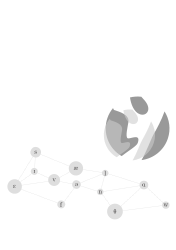
\includegraphics[width=\paperwidth,height=\paperheight]{cover2.pdf}
    \vfill
    }}}


% IPA support
\usepackage{fontspec}
\setmainfont{Doulos SIL}

\usepackage[all]{nowidow}


%% For A4 paper
%\geometry{
%  left=24.8mm, % left margin
%  textwidth=120mm, % main text block
%  marginparsep=8.2mm, % gutter between main text block and margin notes
%  marginparwidth=49.4mm % width of margin notes
%}



%%%% BEGIN - \citett - 
% #1 {, } - #2 { and } - #3 \cmd - #4 list
\makeatletter
\newcommand\textlist[4]{%
  \let\last@item\relax
  \let\last@sep\relax
  \@for\@ii:=#4\do{%
    \ifx\last@item\relax\else
      \ifx\last@sep\relax
        \def\last@sep{#2}%
      \else#1\fi
      #3{\last@item}%
    \fi
    \let\last@item\@ii
  }%
  \ifx\last@item\relax\else
    \last@sep#3{\last@item}%
  \fi
}
\makeatother
\newcommand{\citett}{\textlist{, }{ and }{\citet}}
%%%% END - \citett


%%%% ABSTRACT
\newenvironment{abstract}{\section*{Abstract}\begin{small}}{\end{small}}

%%%% change figure counting 
\usepackage{chngcntr}
\counterwithout{section}{chapter}
\counterwithin{chapter}{part}

\usepackage{multirow}
\usepackage{longtable}
\usepackage[caption=false]{subfig}
\usepackage{lineno}
\linenumbers

\begin{document}

\AddToShipoutPicture*{\BackgroundPic}
% Front matter
\frontmatter

% r.1 blank page
% \blankpage

% v.2 epigraphs
% \newpage\thispagestyle{empty}
% \openepigraph{%
% The public is more familiar with bad design than good design.
% It is, in effect, conditioned to prefer bad design, 
% because that is what it lives with. 
% The new becomes threatening, the old reassuring.
% }{Paul Rand%, {\itshape Design, Form, and Chaos}
% }
% \vfill
% \openepigraph{%
% A designer knows that he has achieved perfection 
% not when there is nothing left to add, 
% but when there is nothing left to take away.
% }{Antoine de Saint-Exup\'{e}ry}
% \vfill
% \openepigraph{%
% \ldots the designer of a new system must not only be the implementor and the first 
% large-scale user; the designer should also write the first user manual\ldots 
% If I had not participated fully in all these activities, 
% literally hundreds of improvements would never have been made, 
% because I would never have thought of them or perceived 
% why they were important.
% }{Donald E. Knuth}


% r.3 full title page
\maketitle


% v.4 copyright page
\newpage
\begin{fullwidth}
~\vfill
\thispagestyle{empty}
\setlength{\parindent}{0pt}
\setlength{\parskip}{\baselineskip}
Copyright \copyright\ \the\year\ \thanklessauthor

\par\smallcaps{Published by \thanklesspublisher}

%\par\smallcaps{tufte-latex.googlecode.com}

\par Licensed under the Apache License, Version 2.0 (the ``License''); you may not
use this file except in compliance with the License. You may obtain a copy
of the License at \url{http://www.apache.org/licenses/LICENSE-2.0}. Unless
required by applicable law or agreed to in writing, software distributed
under the License is distributed on an \smallcaps{``AS IS'' BASIS, WITHOUT
WARRANTIES OR CONDITIONS OF ANY KIND}, either express or implied. See the
License for the specific language governing permissions and limitations
under the License.\index{license}

\par\textit{First printing, \monthyear}
\end{fullwidth}

% r.5 contents
\tableofcontents

%\listoffigures

%\listoftables

%% r.7 dedication
%\cleardoublepage
%~\vfill
%\begin{doublespace}
%\noindent\fontsize{18}{22}\selectfont\itshape
%\nohyphenation
%Dedicated to those who appreciate \LaTeX{} 
%and the work of \mbox{Edward R.~Tufte} 
%and \mbox{Donald E.~Knuth}.
%\end{doublespace}
%\vfill
%\vfill


% r.9 introduction
\cleardoublepage
\chapter*{Introduction}
EICEFALA is an event promoted by UFMG laboratories from Faculdade de Letras
(Laboratório de Fonologia) and Escola de Engenharia (CEFALA).

The comprehension of human communication involving speech acoustics and
gestures requires knowledge from various fields of science, such as phonetics,
phonology, linguistics, acoustics, mechanics, mathematics, physiology,
neuroscience and computer science. The objective of the 7th EICEFALA is to
present and discuss theoretical and methodological techniques to researchers
from the several areas of knowledge working with speech science: linguists,
engineers, physicists, speech therapists, musicians, etc. It is expected that
the participants of the event find, at EICEFALA, a transdisciplinary forum to
address questions related to spoken communication.


%%
% Start the main matter (normal chapters)
\mainmatter

\epigraphhead[450]{Fairy tales are more than true: not because they tell us that dragons exist, but because they tell us dragons can be beaten.\par\hfill\textsc{C.K. Chesterton}}
\part{Plenary Speakers}
{
\chapter{Using statistical learning techniques to determine Cantonese lexical tones from the acoustic and visual components of speech}\label{ch:adriano}
\chapterauthor[1]{João Vitor Possamai de Menezes}
\chapterauthor[1]{Hani Camille Yehia}
\chapterauthor[1]{Adriano Vilela Barbosa}
\begin{affils}
\chapteraffil[1]{Universidade Federal de Minas Gerais}
\end{affils}

\noindent 
This mini-course presents an introduction to the use of statistical learning techniques to speech
processing problems. More specifically, we show how classification techniques can be used to
predict lexical tones in Cantonese from the associated measurements of both the acoustic and the
visual (to a lesser degree) components of speech. The acoustic and visual data we use were recorded
during a speech production experiment where a native speaker of Cantonese produced a set of
words spanning the full range of Cantonese tones. The visual data consists of 3D trajectories of
markers on the subject’s face and head recorded with an Optotrak. The acoustic component is
represented by F0 trajectories extracted from the speech acoustics. The idea is to use the F0 and
marker trajectories as input vectors to train classifiers to predict the lexical tones. However, these
trajectories cannot be used directly because they have different durations for different tokens
(utterances), whereas all input vectors to the classifiers must have the same dimension. In order to
make all input vectors the same length, regardless of the duration of the utterances, all trajectories
(both F0 and markers) are approximated by polynomials of a given order and represented by the
corresponding coefficients. The polynomial coefficients are then used as input vectors to train
different classification models (LDA, SVM, K-nearest neighbors, etc). The performance of the
models is estimated by means of k-fold cross validation. Although the statistical learning techniques
we present are applied to a specific problem (estimating Cantonese lexical tones from the acoustical
and visual components of speech), they are general and can be equally applied to a wide range of
problems. All procedures presented in the mini-course are developed in the R language.

\chapter{The multiple dimensions of speech: old questions and new challenges}\label{ch:didier}
\chapterauthor[1]{Didier Demolin}
\begin{affils}
\chapteraffil[1]{Laboratoire de Phonétique et Phonologie\\CNRS-UMR 7018}
\end{affils}

\noindent 
Human speech, a product of the evolution of primates, can in essence be defined
in terms of a signal. This is an acoustic wave varying over time with amplitude
and frequency modulations, due to the articulatory movements of the vocal
tract’s organs. To perform these movements, motor controls are required, whose
interactions with the aerodynamic parameters produce the acoustic signal. The
main objective of research in this domain is to understand which primary
principles,biological, physical and cognitive, to be based on to explain
the production and perception of speech in the world’s languages and to make the
fundamental question: \textit{how does it work?}

Among the main fields of activity involved in the study of sounds and sound
systems of languages are the engineering sciences with the dimensions of
automatic processing (speech recognition and synthesis);phonetics and phonology
(the linguistic aspects); and pathological aspects(how to explain what doesn't
work anymore or less well). This includes knowledge of similar fundamental
principles. To these dimensions a readded physics, biology, cognition and
neuroscience. These fields involves in-depth knowledge of various
interconnected fields to explain how sounds and sound systems work. Therefore in
addition to the symbolic dimension, anatomical, physiological, acoustic,
aerodynamic, articulatory,auditory, proprioceptive, historical (phylogenies
and diachrony),ecological, temporal, dynamic and self-organized aspects can,
and should,be integrated in the explanation of the studied phenomena.

The complexity and interactions of these dimensions find new light in the
paradigms resulting from the study of complex systems, which makes it possible
to address old issues again, such as the search for a possible speech code,
invariants and primitives. From these issues, others arise, such as the
understanding of the open or closed nature of sound systems, which is far from
being resolved. Explaining the diversity,complexity and dynamics of sound
systems involves understanding the nature of variation in speech phenomena. How
can we show that spontaneous speech, laboratory speech and pathological aspects
are based on the same principles?

The evolution of theory, models, new statistical tools,computational, big data
and deep learning tools, allow these issues to be addressed in a new light. New
measuring instruments such as real-time magnetic resonance imaging, functional
magnetic resonance, three-dimensional or four-dimensional ultrasound, digital
endoscopy,electroencephalography (EEG) and many other recent tools make
it possible to accurately observe, measure and quantify speech phenomena as well
as bring to discussion fundamental issues still unresolved or poorly understood. 

The lecture will discuss the controlled and automatic aspects involved in the
control of breathing in speech, issues in speech embodiment, the quantal
aspects of speech, the importance of thresholds values in aerodynamic and
acoustic parameters, types of feedback (acoustic and proprioceptive) in speech
phenomena and new ways to explain and formalize the source, the initiation and
propagation of sound changes. This last point by using and adapting
population ecology models to speech. 


%\bibliographystyle{plainnat}
%\bibliography{didier.bib}

\chapter{Some questions on L2 speech as related to colonialism}\label{ch:eleonora}
\chapterauthor[1]{Eleonora Albano}
\chapterauthor[1]{Antonio Pessotti}
\chapterauthor[1]{Carla Diaz}
\begin{affils}
\chapteraffil[1]{LAFAPE-IEL-UNICAMP \& CNPq}
\end{affils}

\noindent
The first aim of this talk is to revisit the question of phonetic drift in $L_2$
speechin light of new data and theory. The new data consist of a sizeable set
of acousticphonetic measures of the speech of Quechua and Spanish monolinguals
and bilingualsresiding in Peru. The theoretical innovation draws on two
sources: the relativelyfamiliar concept of accommodation, introduced by \citet{giles1973}
insociolinguistics, and the less familiar concept of
coloniality, introduced by \citep{quijano2000} in sociology. At the same time, it
aims at showing that phonetic analysis basedon gestural phonology can open new
avenues for exploring the relationship betweenthese two concepts as \textit{explanans}
for $L_2$ pronunciation in an ethnically diverseenvironment.

Accommodation refers to a “constant movement toward and away from others, by
changing one’s communicative behavior” \citep{giles2007}. It encompasses
speech and various other communicative behaviors. Moreover, it has a convergent
side -- enhancing similarities between interlocutors -- and a divergent one --
enhancing differences between interlocutors. Both can occur between two or more
people or within and across speech communities. Some acoustic phonetic
parameters have been useful to tap such shifts \citep[e.g., VOT, as in the pioneering work of][]{sancier1997}.

The concept of coloniality refers to “how colonial patterns of power and
inequality exceed the spatial and temporal boundaries of empire and colony”
\citep{roche2019}. It aims at dealing with the epistemology underlying the
pervasive replication of colonial social, economic, and cultural practices in
postcolonial societies \citep{quijano2000}.

We will start by revisiting earlier work on phonetic drift in L2 conducted at
our lab -- \textit{Laboratório de Fonética e Psicolinguística} (LAFAPE). \citet{ramirez2013}
showed that contact situations may exhibit intralinguistic phonetic
drift in both $L_1$ and $L_2$. In turn, \citet{albano2020} reported preliminary
observations of intralinguistic drift attributable to language attrition in
Quechua/Spanish bilinguals residing in Brazil.

We believe that the understanding of the results of both of these works can be
considerably improved by reference to the above-defined concepts. In
particular, some intriguing signs of partial loss of Quechua stop distinctions
shown by the expatriated Peruvians can be interpreted as mistiming of
articulatory gestures converging towards those of the two hegemonic languages
(namely, Spanish and Portuguese).

Then we will move on to inquire how the study conducted in Peru can elucidate
our questions about Quechua/Spanish relations. All data collection on this
topic was part of Carla Diaz's requisites for completing her bachelor and
master’s degrees in linguistics \citep{diaz2018,diaz2021}. 

Carla recorded 10 Spanish monolinguals and 10 Quechua/Spanish bilinguals in
Lima in August 2019. Then she travelled to Cuzco to record 11 monolingual
Quechua speakers, with the help of a bilingual friend specializing in Quechuan
literature.

The corpus, similar to that of \citet{albano2020}, focused on Quechua and
Spanish stop contrasts. The analysis, likewise, employed measurements that have
been used in the description of Quechua: VOT, amplitude of the stop burst, $f_0$,
and $H1-H2$.

The results show that, unlike the residents of Brazil, the residents of Lima
have no trouble distinguishing stops within the Quechua series or
differentiating them from Spanish stops. The remarkable fact is that divergence
from Spanish was more frequent than convergence. Moreover, certain distinctions
were enhanced by shifting the acoustic parameters beyond the values of the
monolingual group.

After Carla defends her thesis, we are planning to conduct finer-grained
analyses considering the linguistic values and attitudes captured by our
sociolinguistic questionnaire. May we succeed in helping unravel the
coloniality issues behind the subtle attempts of Peruvian Quechua speakers at
resisting diglossia and language loss.

\bibliographystyle{plainnat}
\bibliography{eleonora.bib}


\chapter{How to model the influence of orthography on L2 representationswith BiPhon Neural Networks}\label{ch:silke}
\chapterauthor[1]{Silke Hamann}
\chapterauthor[1]{Chao Zhou}
\begin{affils}
\chapteraffil[1]{University of Amsterdam and University of Lisbon}
\end{affils}

\noindent 
Many studies have shown that written forms influence the acquisition of a second language. 
This influence can be helpful, as is the case of the English /æ/-/ɛ/ contrast that is notoriously
difficult for Dutch learners but where the written form can aid in the creation of the distinction
\citep{weber2004,escudero2010}.
But orthography can also cause the
creation of so-called ghost contrasts, which do not exist in the L2, as is the case with the
intervocalic singleton/geminate contrast in the L2 English of Italian speakers \citep{bassetti2017,hamann2018}.

In this talk, we illustrate how such orthographic influences on the creation of L2
representations can be formalized, by this yielding theoretical predictions that can be tested
again in experimental studies. Our formalization is performed with a symbolic neural network
based on the Bidirectional Phonetics-Phonology model \citep{boersma2007} and its extension by a
reading grammar \citep{hamann2017}.

Our main data comes from an experimental study on Mandarin \citep{zhou2020}: 23
L1-Mandarin speakers with no prior knowledge of EP (naïve listeners), representing the initial
stage of L2 acquisition, performed a delayed-imitation task. They were presented with EP
nonce words containing /ɾ/ in intervocalic onset (e.g., parafa) or word-internal coda (e.g.,
parfa), first auditorily, and then with accompanying orthography. Our results show 1) that
participants only produced L1 [ɻ] when exposed to orthography, confirming that the use of
Mandarin rhotic in L2 speech is orthographically driven; and 2) that even at the initial stage
the substitution with Mandarin [ɻ] occurs almost exclusively in coda position, reminiscent of
L2 learners \citep{zhou2017,liu2018}.

\bibliographystyle{plainnat}
\bibliography{silke.bib}




%\chapter{How to model the influence of orthography on L2 representationswith BiPhon Neural Networks}
%\chapterauthor[University of Amsterdam and University of Lisbon]{Silke Hamann and Chao Zhou}
%\label{ch:silke}
%%\chapter{How to model the influence of orthography on L2 representationswith BiPhon Neural Networks}\label{ch:silke}
\chapterauthor[1]{Silke Hamann}
\chapterauthor[1]{Chao Zhou}
\begin{affils}
\chapteraffil[1]{University of Amsterdam and University of Lisbon}
\end{affils}

\noindent 
Many studies have shown that written forms influence the acquisition of a second language. 
This influence can be helpful, as is the case of the English /æ/-/ɛ/ contrast that is notoriously
difficult for Dutch learners but where the written form can aid in the creation of the distinction
\citep{weber2004,escudero2010}.
But orthography can also cause the
creation of so-called ghost contrasts, which do not exist in the L2, as is the case with the
intervocalic singleton/geminate contrast in the L2 English of Italian speakers \citep{bassetti2017,hamann2018}.

In this talk, we illustrate how such orthographic influences on the creation of L2
representations can be formalized, by this yielding theoretical predictions that can be tested
again in experimental studies. Our formalization is performed with a symbolic neural network
based on the Bidirectional Phonetics-Phonology model \citep{boersma2007} and its extension by a
reading grammar \citep{hamann2017}.

Our main data comes from an experimental study on Mandarin \citep{zhou2020}: 23
L1-Mandarin speakers with no prior knowledge of EP (naïve listeners), representing the initial
stage of L2 acquisition, performed a delayed-imitation task. They were presented with EP
nonce words containing /ɾ/ in intervocalic onset (e.g., parafa) or word-internal coda (e.g.,
parfa), first auditorily, and then with accompanying orthography. Our results show 1) that
participants only produced L1 [ɻ] when exposed to orthography, confirming that the use of
Mandarin rhotic in L2 speech is orthographically driven; and 2) that even at the initial stage
the substitution with Mandarin [ɻ] occurs almost exclusively in coda position, reminiscent of
L2 learners \citep{zhou2017,liu2018}.

\bibliographystyle{plainnat}
\bibliography{silke.bib}



%\chapter{How to model the influence of orthography on L2 representationswith BiPhon Neural Networks}\label{ch:silke}
\chapterauthor[1]{Silke Hamann}
\chapterauthor[1]{Chao Zhou}
\begin{affils}
\chapteraffil[1]{University of Amsterdam and University of Lisbon}
\end{affils}

\noindent 
Many studies have shown that written forms influence the acquisition of a second language. 
This influence can be helpful, as is the case of the English /æ/-/ɛ/ contrast that is notoriously
difficult for Dutch learners but where the written form can aid in the creation of the distinction
\citep{weber2004,escudero2010}.
But orthography can also cause the
creation of so-called ghost contrasts, which do not exist in the L2, as is the case with the
intervocalic singleton/geminate contrast in the L2 English of Italian speakers \citep{bassetti2017,hamann2018}.

In this talk, we illustrate how such orthographic influences on the creation of L2
representations can be formalized, by this yielding theoretical predictions that can be tested
again in experimental studies. Our formalization is performed with a symbolic neural network
based on the Bidirectional Phonetics-Phonology model \citep{boersma2007} and its extension by a
reading grammar \citep{hamann2017}.

Our main data comes from an experimental study on Mandarin \citep{zhou2020}: 23
L1-Mandarin speakers with no prior knowledge of EP (naïve listeners), representing the initial
stage of L2 acquisition, performed a delayed-imitation task. They were presented with EP
nonce words containing /ɾ/ in intervocalic onset (e.g., parafa) or word-internal coda (e.g.,
parfa), first auditorily, and then with accompanying orthography. Our results show 1) that
participants only produced L1 [ɻ] when exposed to orthography, confirming that the use of
Mandarin rhotic in L2 speech is orthographically driven; and 2) that even at the initial stage
the substitution with Mandarin [ɻ] occurs almost exclusively in coda position, reminiscent of
L2 learners \citep{zhou2017,liu2018}.

\bibliographystyle{plainnat}
\bibliography{silke.bib}




%\chapter{“One for all, all for one” -- On process-oriented approaches to multilingual phonetic-phonological development}
%\chapterauthor[UFRGS-CNPq]{Ubiratã Kickhöfel Alves and Laura Castilhos Schereschewsky}
%\label{ch:ubirata}
%%\chapter{“One for all, all for one” -- On process-oriented approaches to multilingual phonetic-phonological development}\label{ch:ubirata}
\chapterauthor[1]{Ubiratã Kickhöfel Alves}
\chapterauthor[1]{Laura Castilhos Schereschewsky}
\begin{affils}
\chapteraffil[1]{UFRGS-CNPq}
\end{affils}

\noindent
Research on language development has shown an interconnection of all the
languages in a multilingual system \citep{herdina2001,pereyron2017}.
This assumption defies a traditional ‘L1 – L2 – L3’ linear order of
influence, as changes in any of the language subsystems may have an
impact on all the others. This also reinforces the importance of a dynamic
approach to language attrition, since the L1 itself shows changes over time.
This is a likely possibility in both dominant and non-dominant L1
environments, as revealed by many studies carried out in the Brazilian
scenario \citep{kupske2015,schereschewsky2018,santos2018,alves2019}.

Aiming to express the interconnectedness of language subsystems over
time, process-oriented approaches \citep{lowie2017,lowie2019} 
have given rise to longitudinal accounts of language development.
Longitudinal methods indicate when changes in each one of the language
subsystems start taking place, revealing how data variability affects
development \citep{chang2021}. In this scenario, many dynamic
approaches to data analyses have been proposed in the last few years
\citep{verspoor2011,hiver2019}. Recent
studies carried out in our research group \citep{albuquerque2019,alves2020,schereschewsky2021} 
suggest that moving correlations \citep{verspoor2011b,bulte2020}, Monte
Carlo techniques \citep{verspoor2011,chang2021}
and Change-Point analyses \citep{taylor2000} may highlight the
modifications that take place in each one of the languages of the
multilingual system, besides suggesting an interconnection among them.

In this presentation, we illustrate these points by presenting two studies
that we have carried out at LABICO (Laboratório de Bilinguismo e Cognição),
at Universidade Federal do Rio Grande do Sul (Brazil). In the first study,
\citet{schereschewsky2021} investigated the development of VOT patterns by
five Brazilian participants (L1: Brazilian Portuguese), learners of English (L2)
and French (L3), all of them residing in their native country. These learners
participated in a three-month longitudinal study, with 12 (weekly) data
points. Following an A-B-A account \citep{hiver2019}, instruction
on English aspiration was provided between weeks 4 and 9, in order to
accelerate variability in the learner’s L2. The results show that an increase
in the aspiration rates in English led to changes in the VOT patterns of both
Brazilian Portuguese (L1) and French (L3).

In the second study, Alves (in progress) has investigated the vowel
development process of an Argentinean (L1: Riverplate Spanish) learner of
English (L2) and Brazilian Portuguese (L3) living in Brazil. This learner was
investigated in a time window of one year and took part in 24 data
collections, which were held every fifteen days. Also following an A-B-A
account \citep{hiver2019}, this participant took part in explicit
instruction classes on the pronunciation of Brazilian Portuguese (vowel and
consonants sounds) between data collections 10 and 15. Our preliminary
results show that changes in F1, F2 and duration in the L3 subsystem have
led to modifications in both the learner’s L1 and L2. Besides, all the vowels
in each subsystem showed dynamic relations with one another, thus
reinforcing the importance of studying all the vowel segments in the
developmental process.

Taken together, the results discussed in this presentation not only provide
empirical evidence to the interconnectedness of language subsystems, but
also foster discussions on process-oriented methods of language
development, as new methodological challenges are highlighted.


\bibliographystyle{plainnat}
\bibliography{ubirata.bib}

%\chapter{“One for all, all for one” -- On process-oriented approaches to multilingual phonetic-phonological development}\label{ch:ubirata}
\chapterauthor[1]{Ubiratã Kickhöfel Alves}
\chapterauthor[1]{Laura Castilhos Schereschewsky}
\begin{affils}
\chapteraffil[1]{UFRGS-CNPq}
\end{affils}

\noindent
Research on language development has shown an interconnection of all the
languages in a multilingual system \citep{herdina2001,pereyron2017}.
This assumption defies a traditional ‘L1 – L2 – L3’ linear order of
influence, as changes in any of the language subsystems may have an
impact on all the others. This also reinforces the importance of a dynamic
approach to language attrition, since the L1 itself shows changes over time.
This is a likely possibility in both dominant and non-dominant L1
environments, as revealed by many studies carried out in the Brazilian
scenario \citep{kupske2015,schereschewsky2018,santos2018,alves2019}.

Aiming to express the interconnectedness of language subsystems over
time, process-oriented approaches \citep{lowie2017,lowie2019} 
have given rise to longitudinal accounts of language development.
Longitudinal methods indicate when changes in each one of the language
subsystems start taking place, revealing how data variability affects
development \citep{chang2021}. In this scenario, many dynamic
approaches to data analyses have been proposed in the last few years
\citep{verspoor2011,hiver2019}. Recent
studies carried out in our research group \citep{albuquerque2019,alves2020,schereschewsky2021} 
suggest that moving correlations \citep{verspoor2011b,bulte2020}, Monte
Carlo techniques \citep{verspoor2011,chang2021}
and Change-Point analyses \citep{taylor2000} may highlight the
modifications that take place in each one of the languages of the
multilingual system, besides suggesting an interconnection among them.

In this presentation, we illustrate these points by presenting two studies
that we have carried out at LABICO (Laboratório de Bilinguismo e Cognição),
at Universidade Federal do Rio Grande do Sul (Brazil). In the first study,
\citet{schereschewsky2021} investigated the development of VOT patterns by
five Brazilian participants (L1: Brazilian Portuguese), learners of English (L2)
and French (L3), all of them residing in their native country. These learners
participated in a three-month longitudinal study, with 12 (weekly) data
points. Following an A-B-A account \citep{hiver2019}, instruction
on English aspiration was provided between weeks 4 and 9, in order to
accelerate variability in the learner’s L2. The results show that an increase
in the aspiration rates in English led to changes in the VOT patterns of both
Brazilian Portuguese (L1) and French (L3).

In the second study, Alves (in progress) has investigated the vowel
development process of an Argentinean (L1: Riverplate Spanish) learner of
English (L2) and Brazilian Portuguese (L3) living in Brazil. This learner was
investigated in a time window of one year and took part in 24 data
collections, which were held every fifteen days. Also following an A-B-A
account \citep{hiver2019}, this participant took part in explicit
instruction classes on the pronunciation of Brazilian Portuguese (vowel and
consonants sounds) between data collections 10 and 15. Our preliminary
results show that changes in F1, F2 and duration in the L3 subsystem have
led to modifications in both the learner’s L1 and L2. Besides, all the vowels
in each subsystem showed dynamic relations with one another, thus
reinforcing the importance of studying all the vowel segments in the
developmental process.

Taken together, the results discussed in this presentation not only provide
empirical evidence to the interconnectedness of language subsystems, but
also foster discussions on process-oriented methods of language
development, as new methodological challenges are highlighted.


\bibliographystyle{plainnat}
\bibliography{ubirata.bib}


%\chapter{Neurophysiological correlates of phonemic categorization}
%\chapterauthor[Laboratory of Psycholgy and Neurocogtion -- CNRS]{Rafael Laboissière}
%\label{ch:rafael}
%\chapter{Neurophysiological correlates of phonemic categorization}\label{ch:rafael}
\chapterauthor[1]{Rafael Laboissière}
\begin{affils}
\chapteraffil[1]{Laboratory of Psycholgy and Neurocogtion -- CNRS}
\end{affils}

\noindent
Speech perception involves the mapping of a continuous, variable acoustic signal of speech into discrete, linguistically meaningful units. This process is known as phonemic categorization. The great variability of the speech signal is caused, among other factors, by coarticulatory phenomena in the speech production process and by communication context effects. Over the past thirty years, great strides have been made in understanding the neurophysiological basis of speech perception from neuroimaging studies of the human brain.  However, it is not clear at what stage of the auditory processing the representations of speech sound cease to be veridical, i.e., faithfully encoding fine acoustic details, and become categorical, i.e., encoding sounds into phonemic categories. It is commonly assumed that in the cochlea, in the brainstem, and in the thalamus, the auditory system processes speech sounds without differentiating them from other types of non-linguistic sound. At some point, however, the central nervous system must treat speech sounds in a special way. In this presentation, a review of recent scientific studies will be presented, revealing which regions of the cerebral cortex are involved in recoding the acoustic waveform into a more abstract phonemic representation, resulting in categorical perception. The results linked to the bilateral asymmetry of categorical perception, as well as the relationship with cortical speech processing models (à la Hickok \& Poeppel) will also be presented. Finally, the principles and limits of behavioral (phonemic identification and discrimination), computational (machine learning), and neurophysiological (electroencephalography - EEG, magnetoencephalography - MEG, functional magnetic resonance imaging - fMRI) methodologies will also be presented.


}

%\epigraphhead[450]{Just because something doesn't do what you planned it to do doesn't mean it's useless.\par\hfill\textsc{Thomas A. Edison}}
%\part{Brazilian Portuguese}

\part{Advances in speech and L2 processing}
{
%\chapter{A pilot study on the prosodic aspects of child-directed signing in Brazilian sign language}\label{ch:marcelomeiraa28}
\chapterauthor[1]{Marcelo Meira Alves}
\chapterauthor[1]{Maria de Fátima de Almeida Baia}
\chapterauthor[1]{Adriana Stella Cardoso}
\begin{affils}
\chapteraffil[1]{Universidade Estadual do Sudoeste da Bahia}
\end{affils}

%%%%%%%%%%%%%%%%%%%%%%%%%%%%%%%%%%%%%%%%%%%%%%%%%%%%%%%%%%%%%%%%%%%%%%

This pilot study investigates the child-directed signing (CDSig) in Brazilian sign language (Libras). To understand the phenomenon CDSig, our research is based on studies on oral languages, such as Elliot (1982), Ferreira (1990),  Fernald (1989), Kuhl (1997), Cavalcanti (1999 ) and Ferreira, Baia and Pacheco  (2019), in which speech alterations are observed at syntactic, discursive, lexical and prosodic levels. Furthermore, regarding the prosodic aspects inherent to CDSig, we support our work on the studies by Holzrichter and Meier (2000) and Fuks (2019) on Israeli and Hebrew sign languages, These studies show that there are phonetic modifications in CDSig, such as displacement, repetitions, stretching and amplification of signs (HOLZRICHTER; MEIER, 2000; FUKS, 2019) as well as the intensification of iconic signs in order to facilitate the communication with their babies in the early stages. We assume the hypothesis that as in oral languages the phenomenon also occurs in Libras as it is a natural human language. To verify the hypothesis, a picture naming experiment was designed with a list of 51 words based on previous studies on child-directed speech (FERGUSON, 1964; STOEL-GAMMON, 1976; CLARK, 2005; BAIA, 2010). The results indicated the occurrence of changes in the phonetic aspects of the sign, such as changes in the movements of the arms and hands, changes in the configuration of the hand, reconfiguration of non-manual expressions, body expressions and iconicity. (Scholarship: FAPESB - 072.4195.2020.0010174-4)

%\chapter{An Exemplar Model in L2 Phonology: a combined approach}\label{ch:danielamarali32}
\chapterauthor[1]{Thaïs Cristófaro-Silva}
\chapterauthor[1]{Daniela Mara Lima Oliveira Guimarães}
\begin{affils}
\chapteraffil[1]{Universidade Federal de Minas Gerais}
\end{affils}

Exemplar Models (EM) have contributed to empirical investigations in Phonology in recent years (Johnson 1997, Pierrehumbert 2001, Bybee 2001). By assuming that phonetic detail is part of phonological representations EM test the gradient implementation of phonetically motivated sound changes. Many contemporary studies point out the challenges  to connect EM approaches to explain L2 learning. This paper intends to explain L2 learning processes by combining EM and the revised Speech Learning Model (SLM-r) proposed by Flege and Bohn (2021). Both models share the assumption that perception and production interact in a dynamic fashion to construct abstract representations. In this paper we add a level of orthography, assuming that mental representations have an impact on L1 and L2 phonological and spelling systems. We claim that L2 acquisition is implemented in a gradient manner where speech production, perception, and orthography operate in an integrated system that models language as a dynamic system. We refer to this proposal as EMPL2: Exemplar Model in L2 Phonology. The major contribution of EMPL2 is to add to Exemplar Models and SLM-r the relevance of detailed phonetic information in shaping L2 phonological representations, besides connecting orthography to linguistic representations. We argue that L2 learners must be offered detailed information about pronunciation and also about the sound-spelling mapping. We hope this combined purpose contributes to better understanding of L2 phonological acquisition, leading to new approaches of teaching pronunciation.

\chapter{An Analysis of the Development of the Rhythm of English-L2 by Brazilian Learners through Rhythmic Metrics and Acoustic Parameters}\label{ch:leonardoanton9}
\chapterauthor[1]{Leonardo Antonio Silva Teixeira}
\chapterauthor[1]{Ronaldo Mangueira Lima Jr.}
\begin{affils}
\chapteraffil[1]{Universidade Federal do Ceará}
\end{affils}

\begin{abstract}
The aim of this study is to describe and discuss the development of L2 English
rhythm by Brazilian learners through rhythmic metrics and prosodic-acoustic
parameters that characterize the oral production of these learners at different
stages of L2 development. Five Brazilian learners of English-L2 were recorded
reading a text in English at the beginning of their college studies in English
Language Teaching, and again four semesters later, after having taken two
English phonology courses. They were also recorded reading a version of the
text translated into Portuguese. Besides the learners, five native speakers of
North American English were recorded reading the same text in English. Data
were manually segmented into vowel units (V), consonant (C), vowel-vowel (VV),
sentences (S) and higher prosodic units - chunks (CH) in PRAAT \citep{boersma_praat},
and the parameters were automatically by means of a script.
Data were statistically treated via R \citep{r2021} %(R CORE TEAM, 2021) 
through the implementation of mixed-effects regression models. Results placed Brazilian
Portuguese and English-L1 in different rhythmic spaces, as predicted by the
literature; in the durational dimension, the metrics positioned the English-L2
of the first recording far from both English-L1 and Brazilian Portuguese; in
the f0 and intensity dimensions, however, the acoustic parameters placed the
English-L2 of the first recording closer to Brazilian Portuguese. In both
dimensions, the English-L2 of the subsequent recording was closer to
English-L1, suggesting a developmental route towards the target language. The
results also suggest positive effects of the explicit teaching of
pronunciation.
\end{abstract}



%%%%%%%%%%%%%%%%%%%%%%%%%%%%%%%%%%%%%%%%%%%%%%%%%%%%%%%%%%%%%%%%%%%%%%
\section{Introduction}
Regarding research in non-native language (L2) development, there seems to be
greater emphasis on segmental aspects rather than prosodic ones \citep{li2014,thomson2015}.
This tendency is also reflected in L2
acquisition models \citep{flege2021,best2007}, 
which emphasize segmental aspects, providing little support to the understanding of L2 prosodic
development. 
%There is also evidence that rhythm can influence the communication
%process in a global way, affecting degrees of perceived foreign accent and
%intelligibility \citep{silva2020}.
Among prosodic features, rhythm is the least explored \citep{cumming2010,gut2012,whitworth_speech_2002},
despite evidence that demonstrates it can influence the communication process in a global way, 
affecting degrees of perceived foreign accent and intelligibility \citep{silva2020}.

The scarcity of studies on the acquisition of L2 rhythm may be related to the
difficulty of establishing the physical reality of such construct. There are at
least three trends on research regarding linguistic rhythm. Lloyd James (1940),
as cited in \citet{abercrombie1971}, relied on the dichotomy Morse code versus
machine gun to illustrate the perceptual difference between English and
Spanish, respectively. \citet{pike1945} formalized that difference by proposing a
rhythmic approach based on the type of units that stood up in such languages:
stress-timed languages, for which interstress intervals would be the most
prominent units, and syllable-timed languages, for which syllables would be
such units. Later, \citet{abercrombie1971} proposed that those rhythmic units would
be isochronous, that is, of the same duration. However, the isochrony paradigm
proved to be empirically unsustainable since intervals of the same duration are
not found in the acoustic signal \citep{cumming2010}.

From the mid-90s, a second trend of studies in linguistic rhythm emerges, in
which the rhythmic patterns are investigated by means of the durational
characteristics of the reference intervals (vowels, consonants, syllables,
etc.), which can be computed by statistical indexes called rhythmic metrics.
\citet{ramus1999} proposed the standard deviation of the duration
of consonantal intervals (ΔC) and the percentual of the total duration of the
utterance composed of vowel intervals (\%V). Those metrics were able to
spatially discriminate languages considered syllable-timed (French, Spanish,
Italian and Catalan), stress-timed (English, Polish and Dutch) and mora-timed
languages (Japanese) \citep{ladefoged1975} on a plane with ΔC and \%V on each axis.%,
%as can be seen in Figure \ref{leo-fig01}, reproduced from the original paper:

%\begin{figure}
%\centering
%\includegraphics[width=0.9\linewidth]{imgs/leo-fig01.png}
%\caption{Distribution of languages over the (\%V, ∆C) plane. Error bars
%represent 1 standard error. Source: \citet[p.~273]{ramus1999}.}
%\label{leo-fig01}
%\end{figure}

The present study follows a third trend on research on linguistic rhythm, which
defines it as a function of the distribution of prominent elements in the
acoustic signal, which involves several acoustic dimensions – duration,
fundamental frequency (f0) and intensity, and may be influenced by the native
language of the speaker \citep{cumming2010,fuchs2016,silva2020}.
Thus, this study was guided by the following questions: (i) how do the metrics
and acoustic parameters place North American English-L1, Brazilian English-L2,
and Brazilian Portuguese (BP)-L1 in the rhythmic space? (ii) What is the
influence of the rhythm of BP-L1 on the development of English-L2 of learners?
(iii) What is the effect of explicit pronunciation teaching on learners'
English-L2 rhythm development? The following hypotheses were raised: (i) PB-L1,
English-L1 and English-L2 are rhythmically different systems; (ii) there will
be rhythmic differences between the English-L2 of the speakers in the two
different stages of development whose recordings were analyzed; (iii) the
English-L2 of the first recording should be more dissimilar to English-L1 due
to L1 transfer and lack of explicit instruction. 

%%%%%%%%%%%%%%%%%%%%%%%%%%%%%%%%%%%%%%%%%%%%%%%%%%%%%%%%%%%%%%%%%%%%%%%
\section{Methods}
As for the participants, the experimental group was composed of five BP-L1
speakers, who were also learners of English-L2. They were all college students
of English Language Teaching, being four men and one woman, aged between 18 to
24. The control group comprised five English-L1 speakers, all Canadians, being
one man and four women, aged 23-34. Four corpora of oral production were
analyzed in this study: English-L1, PB-L1, English-L2 (1) and English-L2 (4).
The data of English-L2 were obtained by means of recordings of the Brazilian
learners reading the first paragraph of a text in two different moments, before
and after completing courses in English Phonetics and Phonology. Those were the
first and fourth recording made so they are referred to as English-L2 (1) and
English-L2 (4). The data of English-L1 resulted from the reading of the same
text by the control group. Finally, the Portuguese-L1 data came from the
reading of the Portuguese version of the text by the Brazilian learners. The
recordings took place in a silent room with a cardioid Shure MX150B lapel
microphone connected to a Zoom 4HnSP recorder. The audio was captured in mono,
with a sampling rate of 44.1 kHz, and saved in wav format.


Data were manually segmented into vowel units (V), consonant (C), vowel-vowel
(VV), that is, the interval between the acoustic onset of a vowel and the onset
of the adjacent one, sentences (S) and higher prosodic units - chunks (CH) in
PRAAT \citep{boersma_praat}, and the script Metrics \& Acoustics Extractor
\citep{silva2020} was used to extract the parameters. Following \citet{silva2020},
the term metric(s) is used in this research to refer
to the duration-based parameters, and the term acoustic parameter(s) refers to
the f0, speech rate and intensive-related ones. The table below presents a
summary of the metrics and acoustic parameters analyzed in this study and the
types of segments they compute:

%%TABLE
\begin{table}
\caption{Rhythm metrics and prosodic-acoustic parameters analyzed in this study}\label{leo-tab01}
\begin{scriptsize}
\begin{tabular}{@{}p{3.1cm}p{1.6cm}p{2cm}p{1.5cm}@{}}
\toprule
\multicolumn{2}{c}{METRICS\protect\footnotemark[1]} & \multicolumn{2}{c}{ACOUSTIC PAREMETERS}\\
Parameters & Segment of application & Parameters & Segment of application \\
\midrule 
Percentual (\%) & V, C & f0 median & S, CH \\
Standard-deviation (∆) & V,C (V ou C), VV & f0 peak & S, CH \\
Variation coefficient (Varco)\protect\footnotemark[2] & V,C (V ou C), VV &  f0 minimum & S, CH \\
Raw pairwise variability index (r-PVI)\protect\footnotemark[3] & V,C (V ou C), VV & f0 standard deviation & S, CH \\
Normalized pairwise variability index (n-PVI)\protect\footnotemark[4] & V,C (V ou C), VV & f0 skewness & S, CH \\
Rhythm ratio (RR)\protect\footnotemark[5] & V,C (V ou C), VV & Mean of f0 first derivative (μΔ1- f0) & S, CH \\
Variability index (VI)\protect\footnotemark[6] & V,C (V ou C), VV & Standard deviation of f0 first derivative (σΔ1- f0) & S, CH \\
\multirow{6}{=}{Yet another rhythm determination (z-score duration) (YARD)\protect\footnotemark[7]} & \multirow{6}{*}{V,C (V ou C), VV} & Skewness of f0 first derivative (skΔ1- f0) & \\
   &  & Speech rate (SR) & VV, S, CH \\
   &  & f0 rate (f0-R)  & S, CH \\
   &  & Spectral emphasis & S, CH \\
   &  & Mean of normalized syllable-peak duration (μdur- Sil) & VV, S, CH \\
   &  & Mean duration of pauses (μdur-\#) & S, CH \\
\bottomrule
\end{tabular}
\end{scriptsize}
\end{table}
\footnotetext[1]{See \citet{fuchs2016} for a comprehensive account of rhythmic metrics.}
\footnotetext[2]{Standard deviation of the segment duration divided by the mean, multiplied by 100.}
\footnotetext[3]{Mean of the differences between successive segments.}
\footnotetext[4]{Mean of the differences between successive segments divided by their sum, multiplied by 100.}
\footnotetext[5]{Mean of pairwise quotients of adjacent segment durations, where the duration of the shorter is divided by the duration of the longer one and multiplied by 100.}
\footnotetext[6]{Mean of the differences between successive segments where the duration of each segment is normalised through division by the mean of all segments’ durations.}
\footnotetext[7]{Mean of the differences between successive segments where the durations are normalised by z-transformation.}

Data were then statistically treated via R \citep{r2021} %(R CORE TEAM, 2021) 
through the implementation of mixed-effects regression models, adopting language and
semester as predictor variables, and rhythmic metrics and acoustic parameters
as response variables.

%%%%%%%%%%%%%%%%%%%%%%%%%%%%%%%%%%%%%%%%%%%%%%%%%%%%%%%%%%%%%%%%%%%%%%%
\section{Results}
In this section, we present some of the significant results, based on the
mixed-effects regression models adjusted for each metric and acoustic
parameter, and the boxplots and bidimensional planes, in which the effect of
each corpus (independent variables) on the significant metrics and acoustic
measures (the dependent variables) can be visually inspected.

\subsection{Metrics}
Twenty out of the thirty employed metrics reached statistical significance for
at least two of the (inter) languages. One example of the mixed-regression
models that were implemented via R can be seen in Table \ref{leo-tab02}, which were adjusted
for the standard deviation of the duration of consonantal intervals (deltaC)
and the percentual of vocalic intervals (\%V).

\begin{table*}
\caption{Coefficients, confidence intervals (95\%) and p-Values for the two
linear mixed-effect regression models adjusted for ΔC and \%V. models: deltaC ~
Lang + (1|Chunk) + (1|Speaker) and percV ~ Lang + (1|Chunk) + (1 /
Speaker).}\label{leo-tab02}
\begin{small}
\begin{tabular}{@{}lllllll@{}}
\toprule
  & ΔC & \%V & & & & \\
Predictors & Estimates & CI & p & Estimates & CI & p \\
\midrule
(Intercept) & 46.48 & 36.17~--~56.79 & \textbf{\textless0.001} & 48.78 & 46.02~--~51.55 & \textbf{\textless0.001} \\
Lang {[}Eng-L1{]} & 21.94 & 7.35~--~36.52 & \textbf{0.004} & -9.66 & -12.97--~-6.35 & \textbf{\textless0.001} \\
Lang {[}Eng-L2 (1){]} & 58.71 & 44.13~--~73.30 & \textbf{\textless0.001} & -11.92 & -14.23~--~-9.61 & \textbf{\textless0.001} \\
Lang {[}Eng-L2 (4){]} & 37.61 & 23.02~--~52.19 & \textbf{\textless0.001}& -9.28 & -11.47~--~-7.09 & \textbf{\textless0.001} \\
\bottomrule
\end{tabular}
\end{small}
\end{table*}


Figure 2 shows the distribution of the 4 corpora over the planes formed by the
pairs ∆C-\%V and VarcoC-VarcoV in comparison to the data reviewed and obtained
by Arvaniti (2012). 

\begin{figure}
\centering
\subfloat[\label{leo-fig02-1}]{\includegraphics[width=0.7\textwidth]{imgs/leo-fig02.png}}\\
\subfloat[\label{leo-fig02-2}]{\includegraphics[width=0.7\textwidth]{imgs/leo-fig03.png}}\\
\caption{Present study data (dark blue) amid all the data reviewed and obtained
by Arvaniti (2012) (light blue) for ΔC - \%V (Figure \ref{leo-fig02} (a) and
VarcoC-VarcoV (Figure \ref{leo-fig02} (b)), in which Eng = English, Ger = German,
Gre = Greek, Spa = Spanish, UI = Italian, Kor = Korean. Source: Teixeira and Lima Jr. (2021).}
\label{leo-fig02}
\end{figure}


As can be seen in Figure \ref{leo-fig02} (a), English-L1 presented greater standard deviation
of consonantal intervals duration (ΔCEng-L1 = 68.41) compared to BP (ΔCBP =
46.48); and BP presented greater proportion of the utterance composed of vowel
intervals (\%VBP = 48.56) compared to English-L1 (\%VEng-L1 = 38,88). The data
of English-L2 (1) were positioned far from the two native languages, scoring ΔC
values quite high (ΔCEng-L2 (1) = 105.19) and the lowest proportion of vowel
segments (\%VEnglish-L2 (1) = 36.24). On the other hand, English-L2 (4) values
were much closer to English-L1 in relation to both axis (ΔCEngl-L2(4) = 84.08;
\%VEng-L2(4) = 39.28). As for VarcoC-VarcoV (Figure \ref{leo-fig02}),
English-L1, English-L2 (1), English-L2 (4) and BP were distributed analogously
to the plane ΔC-\%V, with the BP data recording the lowest values for both the
VarcoC (49.84) and VarcoV (49.04) axis, and English-L2 (1) presenting the
highest scores both in the VarcoC axis (66.8) and in relation to the VarcoV
axis (58.8). The fact that English-L2(1) assumed values far from the L1 (BP)
indicates no objective transference of durational prosodic patterns to the
learners’ interlanguages. On the other hand, the approximation between
English-L2(4) and English-L1 indicates a possible effect of explicit
instruction, among other factors, that may have influenced the temporal
(re)organization of the learners’ speech towards the prosodic patterns of the
target language. 

Regarding the data from Arvaniti (2012), BP grouped with languages considered
more syllable-timed, that is, with more durational regularity among the
segments of reference, such as Spanish and Italian. English-L1 results were
also consistent with the literature, gathering with the results for English and
German from other studies, which are considered languages with more
stress-timing tendency. 

The hierarchy of values for VarcoV-VarcoC and ΔC-\%V illustrates the dominant
positioning pattern for the significant metrics, as can be seen in Table \ref{leo-tab03}:
([+stress-timed] English-L2 (1) > English-L2 (4) > English-L1 > BP [+
syllable-timed]), except for \%V and RR, whose higher values indicate a
tendency towards syllable-timing.

\begin{table*}
\caption{Absolute means for the statistically significant metrics and standard
deviation (between parentheses) for BP, English-L1, English-L2 (1),
English-L2(1) and English-L2(4).\\$^\ast$ S stands for the phonetic syllable, which is the  vowel-vowel (VV) unit.}\label{leo-tab03}
\begin{small}
\begin{tabular}{@{}lllll@{}}
\toprule
Metric & BP & English-L1 & English-L2(1) & English-L2(4) \\
\midrule
\%V & 48.56 (3.16) & 38.88 (4.96) & 36.24 (5.36) & 46.48(8.02) \\
\%C & 51.44 (3,16) & 61.12 (4.96) & 63.76 (5.36) & 68.416(14.55) \\
∆V & 40.08 (10.81) & 41.16 (11.82) & 51.81 (12.79) & 105.192(32.6) \\
∆C & 46.48 (8.02) & 68.41 (14.55) & 105.192 (32.6) & 84.088(36.51) \\
∆S$^\ast$ & 133.4 (45.27) & 198.53 (77.44) & 217.46(97.65) & 184.75 (56.72) \\
VarcoV & 49.04 (8.49) & 54.80 (12.52) & 58.80 (11.30) & 56.32(14.81) \\
VarcoC & 49.84 (7,00) & 59 (11.89) & 66.80 (13.69) & 59.72(22.02) \\
rPVI-V & 65.1 (11.71) & 70.74 (14.84) & 96.98 (19.27) & 81.21(15.75) \\
rPVI-C & 48.22 (8.91) & 86.16 (20.23) & 116.84 (46.64) & 88.7(21.69) \\
rPVI-VC & 64.73 (18.72) & 83.58 (11.12) & 114.4 (38.18) & 89.1(14.53) \\
rPVI-S & 102.85 (40.24) & 130.66 (33.59) & 176.27 (90.03) & 137.96(44.62) \\
nPVI-C & 53.96 (7.21) & 68.56 (11.72) & 72.36 (12.14) & 64.84(11.46) \\
nPVI-VC & 59.76 (7.69) & 68.96 (11.09) & 72.6 (9.40) & 65.08(8.12) \\
RR-C & 61.17 (4.36) & 53.13 (6.29) & 50.97 (6.59) & 54.59(6.42) \\
RR-VC & 58.07 (4.35) & 52.8 (5.65) & 50.91 (4.97) & 54.55(4.59) \\
VI-V & 0.818 (0.166) & 0.981 (0.322) & 1.128 (0.302) & 0.894(0.188) \\
VI-V & 0.830 (0.037) & 0.924 (0.049) & 0.929 (0.052) & 0.934(0.059) \\
VI-VC & 0.684 (0.101) & 0.834 (0.157) & 0.859 (0.120) & 0.746(0.116) \\
VI-S & 0.516 (0.120) & 0.606 (0.136) & 0.615 (0.160) & 0.538(0.126) \\
YARD-VC & 0.717 (0.150) & 0.695 (0.133) & 0.869 (0.113) & 0.848(0.123) \\
\bottomrule
\end{tabular}
\end{small}
\end{table*}

%%%%%%%%%%%%%%%%%%%%%%%%%%%%%%%%%%%%%%%%%%%%%%%%%%%%%%%%%%%%%%%%%%%%%%
\subsection{Acoustic Parameters}
Five out of the twelve employed acoustic parameters reached statistical
significance: f0peak, σf0, σΔ1- f0, spectral emphasis (emph) and speech rate
(SR). 

As for the standard deviation of f0 (Figure 3.1), English-L1 presented the
highest standard deviation among the corpora analyzed (σf0Engl-L1 = 3.79),
followed by English-L2(4) (σf0Engl-L2(4) = 3.34), English-L2(1) (σf0Engl-L2(4)
= 2.71) and BP (σf0BP  = 2.62). The results for this parameter suggest a
gradual prosodic development of the learners towards the f0 variation patterns
of the target language. The standard deviation of f0 first derivative (σΔ1-f0)
(Figure 3.2) was also successful in the separation of the L1s and captured a
similar course of development to that found by σf0. The highest mean was scored
by English-L1(σΔ1- f0Eng-L1 = 5.51), the lowest mean was scored by BP (σΔ1-f0PB
= 3.61). The interlanguages registered intermediate values, but the mean
English-L2(4) was much closer to English-L1 (σΔ1-f0Eng-L2(1) = 3.73 <
σΔ1-f0Eng-L2(4) = 4.61).


\begin{figure}
\centering
\subfloat[\label{leo-fig03-1}]{\includegraphics[width=0.7\textwidth]{imgs/leo-fig04.png}}\\
\subfloat[\label{leo-fig03-2}]{\includegraphics[width=0.7\textwidth]{imgs/leo-fig05.png}}\\
\caption{Boxplots of the means σf0 (Figure 3.1) and σΔ1- f0 (Figure 3.2 for
English-L1, English- L2(1), English-L2(4) and BP. The blue dots and lines
represent the means and standard errors respectively.}
\label{leo-fig03}
\end{figure}

The results for the f0 dimension must be interpreted with caution, since there
was an unbalance between male and female participants in both groups (control
group: 1 male, 4 female; experimental group: 4 males, 1 female). In fact, the
correlation between f0 and sex is evident when individual results are taken
into consideration. For instance, in the experimental group, it was observed
that participant N, the only female, is the one that had the highest f0 peak
(97.16), as well as the widest scopes of f0 (f0 peak minus f0 min) for BP
(17.18) and English-L2(4) (19.06). There was also a smaller variation between
the male learners f0 scope of English-L2(1) (A = 12.28; F = 15.68; K = 15.5; L
13.37) and English-L2(4) (A = 12.81; F = 15.09; K = 14.43; L = 15.1), in
comparison to the variation of the female participant, who went from 15.59 to
19.06 in the last recording. 

In the dimension of intensity, as visually demonstrated in Figure 4.1, spectral
emphasis was able to separate the L1s, with the highest mean for English-L1
among the analyzed corpora (emphEng-L1 = 4.34), which was higher than PB
(emphPB = 2.73). If we consider works that show the correlation between
spectral emphasis and phrasal stress \citep{heldner2001}, %(HELDNER, 2001) 
this result suggests that
native English speakers make more effort as an acoustic clue in stress marking
than Portuguese speakers. Regarding the interlanguages, English-L2 (1) obtained
the lowest mean of spectral emphasis, very close to BP values, (emphEng-L2(1) =
2.56), and English-L2 (4) got much closer to English-L1(emphEngl-L2 (4) =
3.23). This indicates L1 transfer at the intensity dimension, and a tendency
towards the prosodic patterns of English-L1 in the last recording.

\begin{figure}
\centering
\subfloat[\label{leo-fig04-1}]{\includegraphics[width=0.7\textwidth]{imgs/leo-fig06.png}}\\
\subfloat[\label{leo-fig04-2}]{\includegraphics[width=0.7\textwidth]{imgs/leo-fig07.png}}\\
\caption{Boxplots of the means spectral emphasis (Figure \ref{leo-fig04} (a)) and speech rate
(Figure \ref{leo-fig04} (b)) for English-L1, English- L2(1), English-L2(4) and BP. The blue
dots and lines represent the means and standard errors respectively.}
\label{leo-fig04}
\end{figure}

As expected, the L1s presented higher speech rates, with BP registering a
higher mean compared to English-L1 (SRPB = 5.22 > SREngl-L1 = 4.43). In
addition, English-L2 (1) presented the lowest speech rate among the corpora
analyzed (SREngl-L2(1) = 3.59) and English-L2(4) registered a slightly higher
mean, closer to English-L1 (SREng-L2(4) = 3.74). The increase in the speech
rate of the interlanguages between the first and last recording may be related
to the effects of explicit instruction.

%%%%%%%%%%%%%%%%%%%%%%%%%%%%%%%%%%%%%%%%%%%%%%%%%%%%%%%%%%%%%%%%%%%%%%
\section{Discussion}
The metrics and parameters positioned BP, English-L1, English-L2 (1) and
English-L2 (4) as rhythmically different systems. There were differences
between the English-L2 of the speakers in the two different stages of
development and different developmental paths were captured as function of the
dimension of prominence.  This developmental path is consistent with the
definition of interlanguage that presents itself as a relatively independent
system of L1 and L2 \citep{li2014}, and with the non-linearity of the L2
development process \citep{lima2019}.

At the durational level, the dominant distribution pattern was ([+ stress-timed]
English-L2 (1) > English-L2 (4) > English-L1 > BP [+ syllable-timed]), with
English-L2(1) assuming the highest means among the four corpora, and
English-L2(4) getting closer values to English-L1. One possible explanation for
such behavior for English-L2(1) is that learners may have mobilized a process
of dissimilation of phonetic categories, displaying exaggerated durational
values to maintain the distinction between L1 and L2, similarly to what is
predicted by the Speech Learning Model for the segmental level \citep{flege1995,flege2021}. %(FLEGE, 1995,FLEGE; BOHN, 2021).

At the f0  dimension, the dominant distribution pattern ([+ f0 variability]
English-L1 > English-L2 (4) > English-L2 (1) > BP [- f0 variability]) placed
English-L1 with the highest means among the 4 corpora and BP with the lowest
means, which suggests English native speakers mobilize more complex and varied
f0 contours in speech. L1 transfer was more salient at the f0 level and seems
to be more persistent among men, which adds to \citet{urbani2012}. A tendency
towards the f0 prosodic patterns of the target language was also identified at
this level and could be an effect of explicit instruction. This effect may have
also influenced the greater speech rate ([+ speech rate] BP > English-L1 >
English-L2 (4) > English-L2 (1) [- speech rate]) and spectral emphasis ([+
spectral emph] English-L1 > English-L2 (4) > BP > English-L2 (1) [- spectral
emph]) for English-L2 (4), suggesting more fluency of the learners, and an
overall improvement in marking syllable stress, respectively.

%%%%%%%%%%%%%%%%%%%%%%%%%%%%%%%%%%%%%%%%%%%%%%%%%%%%%%%%%%%%%%%%%%%%%%
\section{Conclusion}
The metrics and acoustic parameters confirmed the first hypothesis that North
American English-L1, Brazilian English-L2, and BP-L1 are rhythmically
different systems. We confirmed the hypothesis that the data of English-L2 (1)
would be more dissimilar in relation to English-L1 compared to the data of
English-L2 (4), but orthogonal patterns of rhythmic development seem to coexist
as a function of the different dimensions of prominence. Nevertheless, the
approximation between the means of English-L2(4) and English-L1 in all
dimensions suggest positive effects of explicit pronunciation in the
development of prosodic features by learners of non-native languages.  As
future work, we intend to expand the analyzed corpora including the recordings
of the 2nd and 3rd semesters as well as the other paragraphs of the text, and
to analyze the correlation between the metrics and acoustic parameters and
perceived degrees of foreign accent, intelligibility, and comprehensibility.  



\section{Acknowledgment}

This study integrates a project that is partially financed by CNPq, process 438823/2018-4.

%%%%%%%%%%%%%%%%%%%%%%%%%%%%%%%%%%%%%%%%%%%%%%%%%%%%%%%%%%%%%%%%%%%%%%
\bibliographystyle{plainnat}
\bibliography{leonardoanton9.bib}



\chapter{Change-Point Analysis in language development: a study of voice onset time production in a multilingual system}\label{ch:adrielledecar3}
\chapterauthor[1,2]{Laura Castilhos Schereschewsky}
\chapterauthor[1,3]{Ubiratã Kickhöfel Alves}
\begin{affils}
\chapteraffil[1]{Universidade Federal do Rio Grande do Sul}
\chapteraffil[2]{CAPES}
\chapteraffil[3]{CNPq}
\end{affils}

%%%%%%%%%%%%%%%%%%%%%%%%%%%%%%%%%%%%%%%%%%%%%%%%%%%%%%%%%%%%%%%%%%%%%%
\section{Introduction}


According to Complex Dynamic Systems Theory (CDST) \citep{larsen-freeman2008,cameron2008,lowie2015,lowie2019},
when it comes to
multilingual development, we need to think about the interconnectedness of the
system components. Departing from this assumption, we follow Kupske's concept
of language attrition\footnote{In this paper, we do not differentiate ‘language
attrition’ from ‘language transfer’ or ‘language drift’. We will use the three
terms interchangeably.}, which characterizes this phenomenon as the force
resulting from the contact of two bodies, in this case, two languages, that are
in constant movement \citep[p.~39--40]{kupske2016}. This concept embraces the
CDST premise that change is inherent to development. Thus, if the system is in
constant movement, we may find it in continuous change in a given state, and
language variability is expected to be found. Sometimes, the system may go
through significant changes that exceed its current state \citep{van_dijk2007}.
If these particular changes lead to the reorganization of the
system as a whole (as in the emergence of a new attractor state), we call them
‘phase transitions’ or ‘phase shifts’. According to \citet{hepford2020}, this new
attractor state is not necessarily something new to learners, as it "could be a
language form that they are exposed to regularly but have not had the cognitive
ability to adapt to, or an event that pushes a learner to adapt and
self-organize resulting in using a new form" \citep[p.~162--163]{hepford2020}.

Based on the aforementioned assumptions, this study aims to investigate the
phenomena that occur in the development of the additional languages of
trilingual speakers, native speakers of Brazilian Portuguese (BP-L1) and
non-native speakers of English (L2) and French (L3). Specifically, this
longitudinal study analyzes, over a period of three months (with 12 weekly
datapoints), the development of the production of Voice Onset Time (VOT),
observing possible phase shifts through change-point analyses \citep[cf.]{taylorwayne}
provided by the Change-point analyzer v.2.3 software \citep{taylor-analyzer}. 
The study included a period of pedagogical intervention to accelerate
the development of the positive VOT pattern with the characteristic aspiration
of English. This teaching intervention took place over six explicit
pronunciation instruction sessions, conducted in the weeks of datapoints 4 to
9. We aimed to discuss to what extent the accelerated development of an L2 with
a typologically different VOT pattern causes changes in the development of the
L3 and L1 subsystems, as well as show the inter-relation of the two additional
languages over time.

According to the literature \citep[cf.]{schereschewsky2021}, from the study of VOT,
we can observe the multidirectionality of transfer and the adaptability and the
self-organization of language subsystems. Therefore, this study intends to
provide empirical and theoretical input into a larger  understanding of these
aspects. This may shed light on the development of additional languages in the
light of CDST. As this is essentially a theory about change, we aim to raise
issues such as language development and its ongoing "process" in time \citep[cf.]{lowie2015,lowie2019},
the interconnectivity of typologically different
subsystems, data variability, and the emergence of new attractor states and
phase shifts.


%%%%%%%%%%%%%%%%%%%%%%%%%%%%%%%%%%%%%%%%%%%%%%%%%%%%%%%%%%%%%%%%%%%%%%
\section{Method}
As addressed in the previous section, the main goal of this study was to
inferentially verify possible phase shifts in VOT patterns, in each of the
language subsystems, especially after the beginning of explicit pronunciation
instruction in English. For that, we carried out change-point analyses \citep[cf.]{taylorwayne}.

In order to achieve our goal, we proposed a methodology in which changes and
interactions among the subsystems of multilingual speakers could be
investigated through accelerating L2 VOT development. The experiment was built
with a longitudinal design in an A-B-A format \citep[cf.]{hiver2020},
with 12 datapoints, which were intersected in the midpoints with 6 sessions of
explicit pronunciation instruction in English. This intervention took place
between the weeks referring to datapoints 4 and 9, and all instructional
sessions were conducted with a communicative approach.

In this study, we replicated different process-oriented analyses to encompass
and address variability \citep{garcia2013}, conducting the same experiment with
five participants from different backgrounds, different ages, with different
proficiency levels in their additional languages, and different routines. Due
to space restrictions, in this paper we will focus on the results from one
particular participant\footnote{This participant is referred to as Participant
5 in previous works from this project. For more information on the other
participants, see \citet{schereschewsky2021}.}, who was 24 years old at the time, a
graduate student who worked as a French teacher. This participant took a
self-evaluation test \cite{schereschewsky2021}%\citep{scholl2013}%(SCHOLL; FINGER, 2013) 
and graded herself a 6 in English
and a 10 in French\footnote{It is interesting to note that her L3 was more
active than her L2, because she worked as a French teacher, even though she had
started studying English before she even started learning French.}.

The participant was presented with three different reading tasks. In each data
collection session, she received 23 carrier sentences (repeated three times
each) with 18 target words with /p/, /t/ and /k/ in word-initial position and 5
distractor words. The BP and English instruments were the same as in Kupske
(2016), for both matters of consistency and comparisons of results with
previous studies. We also used the same methodological control as Kupske in the
development of the French instrument \citep[cf.]{schereschewsky2021}. Because she
received the same target words, the order of the carrier sentences was
randomized and the distractor words were changed each week. This study was
conducted during the pandemic of COVID-19, so the participant accomplished the
experiment in an individual setting and was asked to complete each task taking
time intervals between them.

All audio recordings from the reading tasks were analyzed acoustically in the
Praat v.6.1.16 software \citep{boersma2019}. Due to time and space
restrictions, only the absolute values of VOT production were considered. As
for VOT measurements, similar criteria to previous works were used: selecting
the voiceless interval between the burst of the stop consonant and the first
regular pulse of the following vowel.

As for the statistical analyses, the participants' developmental trajectories
were plotted, considering minimum, maximum, and mean values from the tokens of
each stop consonant in each datapoint. Following that, change-point analyses
\citep[cf.]{taylorwayne,steenbeek2012,baba2014,han2018,englhardt2020,henry2021}
were conducted. Change-point analysis is an inferential method that uses resampling
and cumulative sums to identify a pattern shift, or the point of change, in a
set of longitudinal data.

The Change-Point Analyzer software is able to detect several longitudinal
changes. By running a fast analysis of cumulative sums and bootstrapping, for
each change in pattern, the software provides practical information, including
the confidence level, which indicates a probability that a change has actually
occurred, and the confidence interval, which indicates when that change has
occurred. Figure 1 shows the first output tab from the software, with the
change-point analysis visual plot.

\begin{figure}[h]
\centering
\includegraphics[width=0.7\linewidth]{imgs/lauracastilho22-image1.png}
\caption{Outputs - change-point analysis visual plot.} 
\label{laura-fig01}
\end{figure}

In Figure \ref{laura-fig01}, the bold black line in the graph represents the raw data of the
mean VOT values of [p] in Participant 5’s L1 over the 12 collection points. The
dark blue lines represent the amplitude range of the control limits, that is,
the maximum range of variation in which the values can fluctuate, assuming that
no change has occurred (if the black line exceeds the control limits, we will
have a first indicative that a change has taken place, which may simply be an
outlier or an indication of an actual phase shift). The lighter blue background
represents the area that should contain all values varying within the control
limits. The displacement of this area in light blue at the bottom of the graph
actually indicates a phase shift, as the average values within the first
segment show a sudden change, starting to vary in a different range,
represented by the second segment of the area in lighter blue. Figure \ref{laura-fig02} shows
the second output tab from the software, with the significant changes of the
set of data.

\begin{figure}[h]
\centering
\includegraphics[width=\linewidth]{imgs/lauracastilho22-image2.png}
\caption{Outputs - table of significant changes.} 
\label{laura-fig02}
\end{figure}

The table in Figure \ref{laura-fig02} indicates the estimated point of change to another phase,
in this case, in Datapoint \#5, with a confidence level of 97\%\footnote{The
Change-point Analyzer only presents, in the outputs, intervals that have at
least 95\% confidence. The more spaced the confidence interval, the lower the
confidence level for a change to have occurred at the point identified by the
software.}, indicated by the confidence interval (which, in this case, points
exactly to session 5). Next, the table indicates the values before and after
the change, that is, the average values of variation in the first phase
(considering the average of all inputs within this first phase), which go from
34.25ms to 46.29ms in the second phase. Finally, the level of change indicates
its importance. In this particular example, the Level 1 change indicates that
this was the first significant change identified by the software in the first
analysis run of the data. Other change levels may appear, depending on how many
phase changes are identified and whether these are significant. Finally, Figure
\ref{laura-fig03} shows the third output tab from the software, with the visual chart showing
the cumulative sums.

\begin{figure}[h]
\centering
\includegraphics[width=0.7\linewidth]{imgs/lauracastilho22-image3.png}
\caption{Outputs - table of significant changes.} 
\label{laura-fig03}
\end{figure}

The chart in Figure \ref{laura-fig03} represents the cumulative sum analyses (CUSUM).
According to \citet[p.~6]{taylorwayne}, "they are the cumulative sums of differences
between the values and the average". These differences sum to zero so the
cumulative sum always ends at zero. Thus, in the CUSUM graph from this data, a
downward sloping line can be seen, indicating that the values in that period
have a tendency to be below the general average, until there is a change in the
direction of the line, starting to have an upward slope, indicating that values
from that portion of the graph tend to be above the overall mean. We should
also look at the shaded background of the chart, which indicates whether and
where there has been a significant change in the slope of the line, referring
to the table with confidence intervals. Another important information brought
by the CUSUM chart is that the straighter the line, regardless of its direction
(up or down), the greater the certainty that no change occurred in that period.
On the other hand, the more curved the line is, as is the case between points 4
and 9, the greater the possibility that other changes (from other levels) have
taken place.


%%%%%%%%%%%%%%%%%%%%%%%%%%%%%%%%%%%%%%%%%%%%%%%%%%%%%%%%%%%%%%%%%%%%%%
\section{Results}

As previously mentioned, change-point analyses are used to identify the points
at which a pattern change occurs in a longitudinal dataset. Thus, change-point
analyses help identify the developmental stages of VOT production, checking
attractor states in phases of relative stability in each language. In this
section, only a summary of the significant changes and the most relevant charts
for the discussion will be presented. A table will presented for each language,
with the significant results split by consonant (/p, t, k/), of the data
collection session the change took place, the confidence interval, the
confidence level (in percentages), the mean values before and after the change
(which is related to the averages of variation of values within the control
limits of each phase) and the level of change (degree of importance in the
analysis by the software). Table 1 shows the results of Brazilian
Portuguese-L1.

\begin{table}[h]
\caption{Change-point analysis of BP-L1.}\label{laura-table01}
\begin{tabular}{@{}lllllll@{}}
\toprule
\textbf{Stop} & \textbf{Measure} & \textbf{Session} & \textbf{Conf.level} & \textbf{From} & \textbf{To} & \textbf{Shift} \\
\midrule
{[}p{]} & Mean & 5 & 97\% & 34,252 & 46,289 & ↗ \\
{[}p{]} & Max & 5 & 95\% & 69,097 & 84,571 & ↗ \\
{[}t{]} & Mean & 11 & 100\% & 40,181 & 32,775 & ↘ \\
{[}t{]} & Max & 11 & 99\% & 76,253 & 48,585 & ↘ \\
{[}k{]} & Mean & 4 & 96\% & 59,073 & 75,531 & ↗ \\
\bottomrule
\end{tabular}
\end{table}

First, we emphasize the interconnectedness of the language subsystems, which
makes it possible for a native language to change, even if it is typologically
different from a language that underwent an intervention, as we found
significant phase changes in the production of VOT in Portuguese-L1 in the
three stops.

For [p], we found a Level 1 phase shift in the means in Datapoint 5, when the
averages change from 34.25ms to 46.29ms, and a Level 3 change in maximums
around Datapoint 5, when the averages increase from 69.1ms to 84.57ms.

For [t], in which we also found significant phase changes in the averages and
maximum instances, the data are somewhat more interesting. In both measures,
Level 2 phase changes are found, in which the VOT decreases in duration. For
the means, phases shifted from an average of 40.18ms to 32.78ms. For the
maximum instances, they shifted from 76.25ms to 48.59ms. However, as both
changes are Level 2 and this new phase with shorter VOT measures only starts by
the end of the analyzed period, around Datapoint 11, it is also necessary to
visually analyze these data, since there is also the possibility that another
(non-significant) change occurred in previous datapoints. Figure
\ref{laura-fig04} shows the change-point analysis plots for the two measures.

\begin{figure}[h]
\centering
\subfloat[\label{laura-fig04-1}]{\includegraphics[width=0.45\textwidth]{imgs/lauracastilho22-image4.png}} \qquad
\subfloat[\label{laura-fig04-2}]{\includegraphics[width=0.45\textwidth]{imgs/lauracastilho22-image5.png}} \\
\subfloat[\label{laura-fig04-3}]{\includegraphics[width=0.45\textwidth]{imgs/lauracastilho22-image6.png}} \qquad
\subfloat[\label{laura-fig04-4}]{\includegraphics[width=0.45\textwidth]{imgs/lauracastilho22-image7.png}} 
\caption{Change-point analysis of means and maximum instances of [t] in Portuguese-L1.}
\label{laura-fig04}
\end{figure}

The graphs of the means and the maximum instances of [t] show that the two
measures presented a very similar behavior during the analyzed period.
Comparing the initial and final points of the measurements, there is a clear
trend towards a decrease in the descriptive values of VOT, which is in
accordance with the phase shift found with a decrease of averages. However,
there is also a very clear indication that the data may have undergone another
phase shift, around Datapoint 3, where the VOT appears to have increased in
duration. The CUSUMs graph shows the possibility of another phase shift due to
the sudden change in the direction of the cumulative sums line on the third
datapoint. However, the software did not verify this change as significant to
include it in the outputs. What was included in the outputs was a significant
Level 1 phase shift in the means of [k], where there was an increase in the
averages from 59.07ms to 75.53ms in Datapoint 4, thus after the beginning of
the intervention, once again showing that even the subsystem of a typologically
different language is subject to change as a result of another one changing.


\begin{table}[h]
\caption{Change-point analysis of English-L2.}\label{laura-table02}
\begin{tabular}{@{}lllllll@{}}
\toprule
\textbf{Stop} & \textbf{Measure} & \textbf{Session} & \textbf{Conf.level} & \textbf{From} & \textbf{To} & \textbf{Shift} \\
\midrule 
{[}p{]} & Mean & 4 & 97\% & 54,553 & 95,416 & ↗ \\
{[}p{]} & Max & 4 & 94\% & 104,37 & 142,81 & ↗ \\
{[}t{]} & Min & 12 & 91\% & 40,409 & 26,24 & ↘ \\
{[}t{]} & Mean & 4 & 94\% & 62,407 & 105,89 & ↗ \\
{[}t{]} & Mean & 11 & 93\% & 105,89 & 80,07 & ↘ \\
{[}t{]} & Max & 4 & 100\% & 110,1 & 147,2 & ↗ \\
{[}k{]} & Mean & 4 & 99\% & 82,73 & 112,96 & ↗ \\
{[}k{]} & Max & 5 & 91\% & 130,65 & 157,73 & ↗ \\
\bottomrule
\end{tabular}
\end{table}

The English-L2 results also bring valuable data to the discussion. For [p],
there is a significant change in Datapoint 4, the first after the start of the
intervention. When it comes to the means, the Level 2 phase shift occurs when
the average changes from 54.55ms to 95.42ms. For the maximums, the Level 1
change occurs with an increase of the averages from a phase of 104.37ms to
142.81, with very high values of VOT production for a bilabial stop.


For [t], we found significant phase changes for the three analyzed measures,
but each measure presented a different result. For minimums, for instance, a
Level 3 phase shift occurs around Datapoint 12, with a decrease in averages
from 40.41ms to 26.24ms. With such a large confidence interval, which covers
the entire intervention until the end of the study, in addition to the fact
that it is a Level 3 change, there remains a possibility of another, less
significant phase shift, in some other datapoint in that interval. For the
means, two significant phase changes were identified, one of Level 1, in
Datapoint 4, with an increase in the averages from 62.40ms to 105.89ms, and one
of Level 2 , at the end of the study, around Datapoint 11, this time with a
decrease in averages (much like what happens in her L1) from 105.89ms to
80.07ms, a higher average than in the initial phase. The maximums of [t]
present a third pattern of behavior, with a Level 3 phase shift around
Datapoint 4, with an increase from 110.1ms to 147.2ms in the later phase.

\begin{figure}[h]
\centering
\subfloat[\label{laura-fig05-1}]{\includegraphics[width=0.45\textwidth]{imgs/lauracastilho22-image8.png}} \qquad
\subfloat[\label{laura-fig05-2}]{\includegraphics[width=0.45\textwidth]{imgs/lauracastilho22-image9.png}} \\
\subfloat[\label{laura-fig05-3}]{\includegraphics[width=0.45\textwidth]{imgs/lauracastilho22-image10.png}} \qquad
\subfloat[\label{laura-fig05-4}]{\includegraphics[width=0.45\textwidth]{imgs/lauracastilho22-image11.png}} \\
\subfloat[\label{laura-fig05-5}]{\includegraphics[width=0.45\textwidth]{imgs/lauracastilho22-image12.png}} \qquad
\subfloat[\label{laura-fig05-6}]{\includegraphics[width=0.45\textwidth]{imgs/lauracastilho22-image13.png}} 
\caption{Change-point analyses of the minimums, means and maximums of [t] in English-L2.}
\label{laura-fig05}
\end{figure}

Figure \ref{laura-fig05} shows the plots of the change-point analyses of the
three analyzed measures of [t] in English-L2. Although the three measures show
completely different behaviors in the outputs, as evidenced by the first graph
of each one, the CUSUM graphs of the three are very similar, indicating sudden
changes in the slope of the cumulatives sums line at least twice on
each\footnote{A downward-sloping CUSUM line indicates values below the overall
average, while an upward-sloping line indicates values above the overall
average. A change in the slope of the line represents a change in trend and,
being a significant change, corresponds to a phase shift.}. This
pattern would be indicative of at least three distinct phases during the study,
in which the first phase change would represent an increase in the average VOT
values, and the second a slight decrease, as we verified in the means of [t],
almost always involving the same datapoints. For minimums and maximums,
however, a possible second phase change was not significant, leaving the
observation only for a qualitative discussion. 

Finally, for [k], we found significant phase shifts in the means and in the
maximums, both indicating an increase in VOT values. For the means, the change
occurred in Datapoint 4, where a new phase went from an average of 82.73ms to
112.96ms. For the maximums, the change occurred around Datapoint 5, when the
results show an increase of the averages from 130.65ms to 157.73ms. Overall,
all these English-L2 data are extremely valuable in showing the influence of
explicit instruction in the development of new attractor states, that is, new
phases developing a non-native positive VOT pattern with long-lag aspiration.
Furthermore, these data highlight change as an inherent characteristic of a
developing system, showing that the language remains in motion even after the
end of an intervention. 

\begin{table}[h]
\caption{Change-point analysis of French-L3.}\label{laura-table03}
\begin{tabular}{@{}lllllll@{}}
\toprule
\textbf{Stop} & \textbf{Measure} & \textbf{Session} & \textbf{Conf.level} & \textbf{From} & \textbf{To} & \textbf{Shift} \\
\midrule 
{[}p{]} & Mean & 4 & 97\% & 30,987 & 40,782 & ↗ \\
{[}p{]} & Max & 4 & 96\% & 60,697 & 78,477 & ↗ \\
{[}t{]} & Mean & 4 & 99\% & 33,437 & 40,15 & ↗ \\
{[}t{]} & Max & 4 & 95\% & 58,91 & 70,327 & ↗ \\
{[}k{]} & Mean & 6 & 92\% & 59,452 & 66,256 & ↗ \\
\bottomrule
\end{tabular}
\end{table}

Once again, we can observe significant phase shifts in the three consonants of
a language subsystem that is typologically different from the language that
received explicit instruction during the intervention, showing the
interconnectivity of the system as a whole. Interestingly, all the identified
changes present new phases with an increase in the VOT values in the French
language. For [p], the means and maximums undergo phase shifts in Datapoint 4.
For the means, the Level 2 shift showed a change in the averages from 30.99ms
to 40.78ms. For the maximums, the Level 1 shift  showed changed averages from
60.68ms to 78.48ms. For visualization purposes, the graphs referring to the
phase shifts in the maximums of [p] are in the Figure \ref{laura-fig06}.

\begin{figure}[h]
\centering
\subfloat[\label{laura-fig06-1}]{\includegraphics[width=0.45\textwidth]{imgs/lauracastilho22-image14.png}} \qquad
\subfloat[\label{laura-fig06-2}]{\includegraphics[width=0.45\textwidth]{imgs/lauracastilho22-image15.png}} \\
\caption{Change-point analyses of the maximums of [p] in French-L3.}
\label{laura-fig06}
\end{figure}

For [t], Level 1 phase shifts were also identified in the means and maximums,
occurring around Datapoint 4. For the means, the phase shift indicates an
increase in average from 33.44ms to 40.15ms, and in the maximums, from 58.91ms
to 70.33ms.

On the other hand, finally, we only found a significant phase shift in the
means of [k]. The Level 1 change was identified around Datapoint 6, indicating
an increase in average from 59.45ms to 66.26ms. Again, we reiterate the
subsystem's ability to change under the influence of changes in other
subsystems, especially the L2, since the new phases were always identified from
the beginning of the instruction period in that language.


%%%%%%%%%%%%%%%%%%%%%%%%%%%%%%%%%%%%%%%%%%%%%%%%%%%%%%%%%%%%%%%%%%%%%%
\section{Final Considerations}
We highlight the relevance of change-point analyses in verifying the emergence
of new developmental phases and we emphasize that change-point analyses allow
us to identify more than one change in each language subsystem, as shown in the
L2 data. Considering that changes in a multilingual system are constant and
that even attractor states are not permanent, an analysis of this sort provides
valuable information on the process of multilingual development. As shown in
our results, languages are entangled and interconnected in a multilingual
system, and they influence one another. Finally, we hope to contribute to the
area of language development in the light of Complex Dynamic Systems Theory.
Discussing methods of analysis that verify developmental changes is always
necessary. Specifically, change-point analyses help to identify the emergence
of new stages of development. As a non-linear process, we acknowledge the
fluctuations of the VOT values in the new developmental phase, as it probably
refers to a less strong attractor state, and even the emergence of a third
phase, different from both the initial phase and the phase under the influence
of the pedagogical intervention. These results show that language and learning
are constantly changing, demonstrating the relevance of an approach via CDST,
given that this, after all, constitutes a theory essentially about change.


%%%%%%%%%%%%%%%%%%%%%%%%%%%%%%%%%%%%%%%%%%%%%%%%%%%%%%%%%%%%%%%%%%%%%%
\bibliographystyle{plainnat}
\bibliography{lauracastilho22.bib}



\chapter{Production of English [Cs] clusters by Brazilian speakers: effects of orthography, phonological environment and task type}
\label{ch:wellingtonara4}
\chapterauthor[1]{Wellington Araujo Mendes Junior}
\begin{affils}
\chapteraffil[1]{Federal University of Minas Gerais}
\end{affils}

This study examines the effects of orthography, phonological environment
and task type in the production of English {[}Cs{]} clusters by
Brazilian Portuguese (BP) speakers. Two orthographic patterns were
examined for English nouns whose plural is pronounced as a (stop +
sibilant) cluster. One of the patterns presents two consonants
word-finally - \emph{cups}, \emph{cats}, \emph{ducks} - whereas the
other one presents a silent vowel \textless{}e\textgreater{} between two
consonants: \emph{grapes}, \emph{plates}, \emph{cakes}. The goal was to
assess whether these different orthographic patterns would trigger the
production of an epenthetic vowel. Additionally, it was assessed whether
different phonological environments would influence the voicing property
of the final sibilant. As it is known, word-final English sibilants are
prone to progressive assimilation (e.g. \emph{cups} {[}kʌps{]},
\emph{bags} {[}bæɡz{]}), rather than regressive assimilation -- as it
occurs in BP (\emph{mês} {[}mes{]}, \emph{mês} \emph{anterior} {[}mez
ə̃.te.ɾi.ˈoɾ{]}). An experiment was designed to test the production of
{[}Cs{]} clusters in English nouns and in BP forms undergoing sound
change. Harmonics-to-noise ratio (HNR) was used to measure sibilant
voicing, whereas the presence of epenthetic vowels was assessed
categorically. Results showed that English learners are more likely to
pronounce a vowel when the orthographic pattern is
\textless{}Ces\textgreater{} rather than \textless{}Cs\textgreater{}, and
this occurs regardless of the visual presentation of the words.
Moreover, HNR rates showed that fully voiced sibilants tend to occur in
L2 English when the consonant is both preceded and followed by a vowel.
These findings are discussed in light of the Exemplar Model in L2
Phonology (EML2P) \citep{guimaraes2021,mendesjr2022}. The
analysis based on the EML2P showed that robust patterns from the L1 are
adopted in L2, including fine phonetic detail that reflects subphonemic
properties.

\section{Introduction}
Traditional phonological models assume that English plural suffixes and
third person singular present forms are subject to a phonological rule.The
underlying representation for regular plural and
3\textsuperscript{rd} person singular present is assumed to be /z/ \citep{hayes2011}.
A progressive assimilation rule predicts that if a vowel
or a voiced consonant precedes /z/, the output is {[}z{]}, as in\emph{dogs}
{[}dɒɡz{]}, \emph{trees} {[}triːz{]} and \emph{pies}
{[}paɪz{]}. If a voiceless consonant precedes /z/, it surfaces as{[}s{]}, as in
\emph{cups} {[}kʌps{]}, \emph{cats} {[}kæts{]} and
\emph{ducks} {[}dʌks{]}. Finally, if an alveolar fricative or anaffricate
precede the sibilant, the outcome is {[}ɪz{]}, as in\emph{buses} {[}bʌsɪz{]},
\emph{quizzes} {[}kwɪzɪz{]} and \emph{watches}{[}wɒtʃɪz{]}. However, when we
consider the orthography of English
plural forms, two possible spellings are associated with theaforementioned
sound patterns. Nouns can either end in a consonant
followed by the letter \textless s\textgreater, as in \emph{books}
and\emph{jobs} or the by letters \textless es\textgreater, as in
\emph{cakes} and \emph{cubes.} Brazilian Portuguese, on the other hand,
presents mainly the \textless Ces\textgreater{} pattern, as it occurs
in\emph{cheques }and\emph{ clubes}, whereas only some few nouns present
the \textless Cs\textgreater{} pattern: \emph{biceps},
\emph{forceps},\emph{volts}.

As a consequence of an ongoing sound change, word-final {[}Cs{]}
clusters\footnote{ For the purpose of the present discussion, we refer  to
{[}Cs{]} as any (consonant + sibilant) sequence. However, as it
will be discussed later, the sibilant may be either voiced or  voiceless.}
are currently very productive some Brazilian Portuguese
plural forms: \emph{crepes}, \emph{potes}, \emph{cheques} \citep{soares2016}. The
alternation between {[}Cs{]} \textasciitilde{} {[}Cis{]}
word-finally in BP follows from the reduction and eventual loss ofunstressed
high front vowels when flanked between a consonant and a
word-final sibilant. It seems that such alternation also applies toplural forms
produced by Brazilian speakers of L2 English, as in\emph{cakes} {[}keɪks{]}
\textasciitilde{} {[}'keɪ.kis{]}.

This paper intends to investigate {[}Cs{]} clusters in English regular
plural forms (e.g. \emph{cups} {[}kʌps{]}, \emph{grapes} {[}ɡreɪps{]})produced
by Brazilian speakers of L2 English in an attempt to address
the question of whether an ongoing sound change from the L1 plays a rolein L2
learning. Additionally, we aim to assess how orthographic and
phonological representations are related. Studies on the relationshipbetween
orthography and phonology have increased in recent years
\citep{rafat2015,hamann2017,zhou2021}.
The main research questions in this topic aim to explain how
L2 learners mediate the relationship between the already knownphonological and
orthographical knowledge from the L1 in order to buildan L2. Thus, an important
question we pose is whether differentorthographic patterns trigger different
pronunciations of {[}Cs{]}
clusters in L2 English.

This paper is organized as follows. The next section reviews studies on
the production of English {[}Cs{]} clusters by Brazilian speakers. Thethird
section describes the methodology adopted in this study. The
fourth section discusses our findings and is followed by theconclusions.



\section{Production of English {[}Cs{]} clusters by Brazilian speakers}
Several works have addressed the relationship between orthography and
the pronunciation of L2 English forms by Brazilian speakers. One of themain
concerns have been to assess whether the presence of an epenthetic
vowel in L2 English is influenced by a letter corresponding to a
vowel. \citet{delatorre2006} investigated the
production of English {[}Cs{]} clusters that occur in past andparticiple forms
by Brazilian speakers of L2 English (e.g. \emph{moved}
and \emph{robbed}). Two epenthetic vowels were attested: one epentheticvowel
breaks up the word-internal consonant cluster and the other one
prevents word-final consonants, as in
\emph{asked}{[}'as.k\textbf{e}.dʒ\textbf{i}{]} and
\emph{saved}{[}'seɪ.v\textbf{e}.dʒ\textbf{i}{]}. \citet{delatorre2006} claimed that
theorthographic input, which was present in a reading task, favored higher
rates of an epenthetic vowel, as opposed to a free speech task, whichdid not
present any orthographic stimulus. Therefore, she argued that
the orthographic input favored the presence of epenthetic vowels in
the pronunciation of L2 English by Brazilian speakers.

Although she did not focus on the
production of {[}Cs{]} clusters, \citet{silveira2007} also investigated
the production of word-final epenthesis in Brazilian speakers of L2 English.
She compared words whose final letter was a consonant (e.g. mad{[}mæd{]}) to
words whose final letter was a silent ⟨e⟩ (e.g.
\emph{made} {[}meɪd{]}). Her results showed that words ending in asilent ⟨e⟩
presented higher rates of epenthesis than words that ended in
a consonantal letter. Akin to \citet{delatorre2006}, the results of \citet{silveira2007}
showed that a reading task favored higher rates of epenthetic
vowels than a free speech task, indicating that orthographic input (and the task
type) contributed to the production of an epenthetic vowel.

Another case of epenthetic vowels reported in the literature involves
word-final consonant and sibilant sequences, {[}Cs{]}, which typically appear in
regular plural and 3\textsuperscript{rd} person singular
present forms in English. It is known that Brazilian speakers of L2English
tended to insert an epenthetic vowel between two word-final
consonants, as it occurs, for example, in \emph{cakes}
{[}keɪks{]}\textasciitilde{} {[}'keɪ.k\textbf{i}s{]} \citep{cristofato2011}.
Interestingly, works that considered 3\textsuperscript{rd} person singular
present and regular plural forms in English spoken by Brazilian
speakers did not account for an epenthetic vowel. They were rather concerned
with voice agreement.

\citet{zanfra2013} studied sibilant voicingin L2 English by Brazilian speakers.
Although her focus was not
specifically on plural forms, her results shed some light on the
current discussion. The author tested whether the BP voicing assimilation rule
involving adjacent segments in word boundaries would apply in L2
English learners' productions. Her results showed that sibilants tended to be
voiced when followed by a voiced consonant (e.g. \emph{The}\emph{hou\textbf{s}e
\textbf{b}ackyard} \emph{is huge}) or by a vowel
(e.g. \emph{The} \emph{mou\textbf{s}e \textbf{I}} \emph{saw is
white}).Conversely, a sibilant was voiceless when the following context was
a pause (e.g. \emph{I won't go if he goe\textbf{s}}.) or a voiceless consonant
(e.g. \emph{The\textbf{s}e pancakes} \emph{are great}). \citet{zanfra2013}
suggested that Brazilian speakers of L2 English speakers transfer the BP
regressive assimilation rule into their L2 English.

\citet{fragozo2017} investigated the
voicing of sibilants in English regular plural forms and 3\textsuperscript{rd}
person singular presented by Brazilian speakers of
L2 English. She assessed the extents to which a sibilant would be voiced after a
voiced consonant, as in \emph{dogs} or \emph{clubs}, which would
reflect the acquisition of a progressive assimilation rule from English.
\citet{fragozo2017} also examined words in context to verify if the
regressive assimilation rule, which applies to BP, would be transferred to L2
English. She found that voiced sibilants tended to follow the
regressive assimilation rule from BP, whereas the English
progressive assimilation rule had a very low rate in her data (0.6\%). She
argues that the low rates of voiced sibilants {[}z{]} in L2 English by Brazilian
speakers follows from the fact that these consonants are only
partially voiced in English. Data from her control group of native speakers
presented 44\% of expected voiced sibilants. Thus, as sibilants
are partially voiced in English, they would not be accessible in L2 English.

\citett{zanfra2013,fragozo2017} both investigated voicing agreement
within a rule-based approach where there would be a competition between a
regressive assimilation rule from BP and a progressive assimilation
rule from English. A question that arises from this assumption is whether a rule
that is transferred from the L1 to the L2 could change as
time goes by. Another issue which is polemic lies on the role played
by orthography, as in hou\textless se\textgreater{}\emph{ }or\emph{}bu\textless s\textgreater{} 
\citep{zanfra2013}. Orthography cannot bemodelled
within a rule-based approach as it is not part of Grammar.
Furthermore, the rule-based approach adopted by \citett{zanfra2013,fragozo2017}
neglected the role played by an epenthetic vowel that may intervene between the
two word-final consonants, as in \emph{cakes}{[}keɪks{]} \textasciitilde{}
{[}'keɪ.k\textbf{i}s{]}. Additionally,
they did not account for the gradience of sibilant voicing.

Unlike previous works which adopt rule-based approaches, this paper
models L2 phonology within an Exemplar Model by considering
representation robustness and the role of fine phonetic detail in
shaping mental representations. Within this proposal, orthography is
modelled as part of the linguistic knowledge of literate speakers and
sound patterns display a great range of variability and gradience.


\section{Methodology}
A set of 36 plural nouns ending in a sequence of (stop + sibilant) were
considered in BP. These words present a single orthographic pattern:
\textless Ces\textgreater, as in \emph{cheques} {[}ʃɛks{]}
\textasciitilde{} {[}'ʃɛ.kis{]} `cheques'. For the L2 English case
study, a set of 36 words were selected, where 15 words display the
orthographic pattern \textless Ces\textgreater, as in \emph{grapes}
{[}ɡreɪps{]}, and the other 21 words display the orthographic pattern
\textless Cs\textgreater, as in \emph{maps} {[}mӕps{]}.

The experiment comprised two tasks. The first one consisted of a
picture-counting task in which participants were asked to count and name
the items shown in the pictures. Short carrier sentences that did not
include orthographic stimuli of the target words were given. The second
trial consisted of a reading task. Initially, participants were asked to
read 72 BP sentences aloud. Alike the picture-counting task, BP nouns in
the reading task were followed by either a vowel or a voiceless
consonant. On the other hand, L2 English nouns were followed by either a
vowel or a pause. The overall number of syllables was controlled for
both languages: 4 in English and 12 in BP, considering the deletion of
the {[}i{]} vowel. Sentence-level intonation and the morphological class
of each word were also controlled.

A group of six Brazilians studying at the Federal Center for
Technological Education of Minas Gerais, in the city of Araxá,
participated in this study\footnote{This research has been approved by
the ethics committee from the Universidade Federal de Minas Gerais,
reference number: CAAE: 15116119.9.0000.5149.}. All participants were
high school students who had been taking English classes as part of the
school's curriculum for about~one year. The group consisted of 3~males
and~3~females and their ages ranged from 15 to 17. All participants
displayed either B1 or B2 proficiency levels (intermediate learners) of
the Common European Framework of Reference for Languages.

Due to the recent COVID-19 pandemic, all interactions were performed
remotely. Experiments were recorded with the \emph{Open Broadcaster
Software Studio}~at 48 kHz sampling rate. The obtained recordings were
converted into WAVEform audio format by the software~\emph{Adobe
Premiere 2020}, which was able to maintain the same sampling rate as the
original files. The average time to complete the experiment was 45 minutes. 
A total of 648 tokens were collected for the L2 English study.
For the BP study, 432 tokens were collected. Samples were edited and
manually annotated using Praat~TextGrids \citep{boersma2020}.

Besides assessing the presence or absence of a vowel between {[}Cs{]}
clusters, this research also considered the voice quality of word-final
sibilants. In BP, only voiceless sibilants occur word-finally, unless a
vowel follows it, to which a voiced sibilant occurs. In English, voiced
and voiceless sibilants occur word-finally. When a vowel follows the
sibilant, the voice quality remains as it formerly was (rather that
changing as it occurs in BP). We posited that word-final voiceless
sibilants would be favored in L2 English, as it is the more robust
pattern in L1. We also posited that a voiced sibilant occurs at higher
rates in an intervocalic position: {[}Cis{]} followed by a word-initial
vowel.

Voicing was measured under Harmonics-to-noise ratio. Each token was
extracted to a separate sound object and a harmonicity object was
created, from which the mean harmonicity was calculated, hereafter the
HNR. The details of its calculation can be found in \citet{Boersma93}.
Harmonicity would seem to be a good measurement of voicing since vocal
cord vibration produces ``a complex periodic wave'' \citep[p.~63]{johnson1997}. 
Based on the discussion from Praat's manual, higher values of HNR
should correspond with higher voicing rates.



\section{Results}

Consider Figure \ref{wel-fig1}, which shows the rates of {[}Cs{]} in regular plural
forms in BP and L2 English.

\begin{figure}[h]
\centering
\includegraphics[width=\linewidth]{imgs/wellingfig01.png}
\caption{{[}Cs{]} rates by orthographic patterns.}
\label{wel-fig1}
\end{figure}

The leftmost column shows that regular plural forms in BP, whose
orthography is \textless Ces\textgreater, presented 62\% of a consonant
followed by a sibilant: {[}Cs{]}. That means that when a letter
\textless e\textgreater{} appears in the orthography of BP plural forms,
a vowel is manifested in 38\% of the cases. The two rightmost columns
report data from English spoken by Brazilian speakers. When the
orthography in the plural form is \textless Ces\textgreater, a consonant
followed by a sibilant {[}Cs{]} occurred in 83\% of the cases, whereas
in the cases where the orthography was \textless Cs\textgreater, a
consonant followed by a sibilant occurred in 96\% of the productions.
This result shows that the pronunciation of {[}Cs{]} is more recurrent
when the orthography is \textless Cs\textgreater{} than when the
orthography is \textless Ces\textgreater{} in regular plural forms in
English. In other words, a vowel will appear at higher rates when the
orthographic pattern is \textless Ces\textgreater{} than when it is
\textless Cs\textgreater. Thus, it is more likely that a plural form as
\emph{tapes} will have a vowel pronounced between the last two
consonants than a plural form as \emph{maps}. The difference between the
data presented in the two rightmost columns is statistically significant
for the orthographic patterns (χ2 = 36.113, df = 1, p \textless{} 0.01).
The explanation for such difference lies in the different orthographic
patterns.

We also considered whether different tasks could favor the production of
an epenthetic vowel. According to \citett{delatorre2006,silveira2007},
visual input favors such non-target productions. In our experiment, the
picture-counting task had no orthographic visual input, whereas
orthography was available in the reading task. If \citett{delatorre2006,silveira2007} 
are correct, then we expect that vowels would occur at
higher rates in the reading task than in the picture-counting task in
our experiment. However, no statistically significant differences were
found between the picture-counting task and the reading task (χ2 = 0.66,
df = 1, p-value = 0.41). This shows that it is the orthographic pattern
rather the type of task that favors a vowel to occur in L2 English. Our
claim is that once speakers are literate, orthography is part of their
grammar, i.e., it has a permanent impact on mental representations. The
EML2P model adopted in the current paper differs from \citett{delatorre2006,silveira2007,zanfra2013}
rule-based approach mainly by
assuming that orthography is part of linguistic knowledge and not
external to it.

Another research question we posited regarded the voice quality of the
word-final sibilant in {[}Cs{]} and {[}Cis{]}. This was the main issue
considered by \citet{zanfra2013,fragozo2017} within a rule-based
approach. Their analysis claimed that voicing in L2 English did not
achieve the target rates due to constraints of BP distribution of
sibilants and regressive assimilation. BP only presents voiceless
sibilants word-finally. However, across word-boundaries, BP sibilants
are voiced when followed by a voiced consonant or a vowel: \emph{mês}
{[}mes{]} `month', \emph{mês bonito} {[}mez ˈbo.ni.tu{]} `beautiful
month', \emph{mês anterior} {[}mez ə̃.te.ɾi.ˈoɾ{]} `previous month'. In
this paper, we offer an alternative view to the preceding rule-based
approaches. Within the scope of the EML2P, it is suggested that
generalizations from an ongoing sound change in BP phonology are
transferred into L2 English, where phonetic detail plays an important
role in shaping mental representations. Consider Figure \ref{wel-fig2}.


\begin{figure}[h]
\centering
\includegraphics[width=\linewidth]{imgs/wellingfig02.png}
\caption{HNR per following phonetic environment in L2 English.}
\label{wel-fig2}
\end{figure}

The boxplots in Figure \ref{wel-fig2} show harmonics-to-noise ratio per following
phonetic environment in L2 English. We can see that when the sibilant is
followed by a pause, it tends to be unvoiced, with HNR rates at around 5
decibels. Conversely, when the sibilant is followed by a vowel, voicing
rates are higher. T-test results show that there is a significant
difference in HNR between both following phonetic environments (t = -8.8153, 
df = 821.37, p-value \textless{} 0,01). However, even though
such environments seem to influence voicing rates of the final sibilant,
these rates are still lower when compared to English target forms. To
put it another way, nouns that should be pronounced with a word-final
voiced sibilant present more unexpected voiceless sibilants than voiced
ones. This can be accounted by the fact that only voiceless sibilants
occur word-finally in BP. Learners are likely unaware of the fact the
{[}z{]} should be voiced in accordance with the voice property of the
preceding segment. Now consider Figure \ref{wel-fig3}.

\begin{figure}[h]
\centering
\includegraphics[width=\linewidth]{imgs/wellingfig03.png}
\caption{HNR per preceding phonetic environment in L2 English.}
\label{wel-fig3}
\end{figure}

The boxplots in Figure \ref{wel-fig3} show harmonics-to-noise ratio per preceding
phonetic environment in L2 English. Data is comprised of sibilants
preceded either by an unvoiced consonant, a voiced consonant or an
epenthetic vowel. At first sight, we can see the HNR rates are somewhat
lower when the sibilant is preceded by an unvoiced consonant, and higher
rates occur when the sibilant is followed by voiced consonants and
epenthetic vowels. An analysis of variance (ANOVA) on these scores
yielded significant variation among conditions: F(2,858)=59.99, 
p\textless{} 0.001. A post-hoc Tukey test showed that the group comprised
of unvoiced consonants differed significantly at p \textless{} 0.05; the
voiced consonants group was not significantly different from the
epenthetic vowels group. This result suggests that epenthetic vowels
contribute to higher rates of voicing as much as other voiced segments
in L2 English. Finally, an interaction between both preceding and
following phonetic environments was attested {[}F(2,858)=7.797, p
\textless{} 0.001{]}.

Our results throw some light on the line of research carried out by
\citett{zanfra2013,fragozo2017}, who investigated the sibilant voicing
followed by a vowel within rule-based approaches. We account for the
fact that low HNR (which reflect voiceless sibilants) is recurrent in
regular plural forms in L2 English, as {[}s{]} is the most robust
exemplar in word-final position in BP. We also account for the fact that
the pattern {[}Cis{]} favors a voiced sibilant in L2 English, as voiced
sibilants are favored in similar contexts in BP (i.e., intervocalically). 
This indicates that L1 exemplar patterns, which
reflect subphonemic information, are adopted in the L2. Finally, our
analysis explains why {[}z{]} presents a low rate of production in L2
English spoken by Brazilian speakers: it is an emerging pattern in the
L2, since it has no exemplars from the L1, at least not in word-final
position. It will be through experience that these exemplars will become
robust and more recurrent.



\section{Conclusions}
The aim of this paper was to investigate {[}Cs{]} clusters in English by
Brazilian speakers. Its main contribution was to assess the role of
orthography, phonological environment and task type not only on the
production of epenthetic vowels, but also on the voicing property of the
final sibilant. It also considered the role played by the {[}Cs{]}
\textasciitilde{} {[}Cis{]} ongoing sound change from BP into L2
English. Results showed that the orthographic pattern
\textless Ces\textgreater{} favors the production of an epenthetic vowel
at higher rates that the \textless Cs\textgreater{} pattern. As for the
task type, it was shown that it was not the visual access to
orthographic forms that triggered a vowel to occur, but rather the
orthographic patterns.

It was also shown that HNR is strongly influenced by
phonetic/phonological environments, including preceding epenthetic
vowels, which had not been accounted for in previous studies. We can
assume that {[}z{]} poses a challenge to Brazilian speakers of L2
English due to the fact that it still has no exemplars from L1 in
word-final position.

Concerning the role played by the BP ongoing sound change involving the
{[}Cs{]} \textasciitilde{} {[}Cis{]} alternation, it was shown that
robust patterns from the L1 are adopted in L2, including fine phonetic
detail that reflects subphonemic properties. This sheds light to the
fact that learners not only transfer sounds to the L2, but also
phonological behaviors in which such sounds are subject to (as seen with
how L2 voicing/HNR is influenced by L1 phonological patterns). We can
assume, thus, that better generalizations are posited when the
production of {[}Cs{]} clusters is assessed globally, rather than
accounting for epenthesis and voicing agreement as separate, unrelated
phenomena.


\bibliographystyle{plainnat}
\bibliography{wellingtonara4.bib}



\chapter{Radial Basis Function Artificial Neural Network for Automatic Identification of Interlanguage Transfer Phenomena}\label{ch:atosapollosil18}
\chapterauthor[1]{Atos Apollo Silva Borges}
\chapterauthor[1]{BrunoFerreira de Sousa}
\chapterauthor[2]{Aratuza Rodrigues Silva Rocha}
\chapterauthor[3]{Wilson Júnior de Araújo Carvalho}
\chapterauthor[1]{Fábio Rocha Barbosa}
\chapterauthor[4]{Ronaldo Mangueira Lima Júnior}
\begin{affils}
\chapteraffil[1]{Federal University of Piauí}
\chapteraffil[2]{Faculdade Afonso Mafrense}
\chapteraffil[3]{State University of Ceará}
\chapteraffil[4]{Federal University of Ceará}
\end{affils}

\begin{abstract}
In the recent decades, especially for non-English speaking
countries, the modern and more connected world has increased the urgency in
learning a second language. Among the obstacles for beginners acquiring a new
language are the grapho-phonic-phonological transfer phenomena between the two
language systems, which may undermine their ability to communicate in the
target language. The present work proposes a seed for an intelligent software
designed to help language learners by providing automatic identification of
transfer phenomena produced during their reading process.The algorithm is
centered on a Radial Basis Function Artificial Neural Network (RBF-ANN) trained
to automatically identify transfer processes between Brazilian Portuguese and
English as ForeignLanguage. Five transfer processes already known in the
literature were chosen to demonstrate the concept; however, as an initial
approach, the audio samples used for training the algorithm weresynthetically
generated by the Google Translate™ TTS system. To train the RBF-ANN algorithm
we used the $\textit{f}_0$ mean and the mean of the first two Formant
Frequencies as signal descriptors. The results presented a promising
perspective for the development of a new computer-assisted pronunciation
training software (CAPT) with accessible computational resources for Brazilian
students and language institutes.
\end{abstract}

%%%%%%%%%%%%%%%%%%%%%%%%%%%%%%%%%%%%%%%%%%%%%%%%%%%%%%%%%%%%%%%%%%%%%%%%%%%%%%%%

\section{Introduction}
During the learning of a new language, a process called interphonology is
manifested. Interphonology is characterized as the creation of a linguistic
system different from both the foreign language (L2) and native language (L1),
but presenting characteristics from both languages simultaneously
\citep{rocha_os_2012}. The students in the processes of acquiring fluency on
the second language transfer some of their knowledge of the L1 to the new
language due to the already established structure of the L1. This phenomenon,
which may be manifested during speech or oral reading, it is called
grapho-phonic-phonological knowledge transfer \citep{zimmer_producao_2006}.
The term grapho-phonic-phonological contemplates not only the transference of
phonetic-phonological knowledge but also the transference of the
grapheme-phoneme relationship of one language to the other, in the case of
this work, Brazilian Portuguese (BP) as L1 to the English as Foreign Language
(EFL), the L2. When the learner finds an unknown structure in the foreign
language, it uses strategies to adapt L2 to a structure already known in L1.

Transfer phenomena between Portuguese as L1 and English L2 produced by
Brazilian learners are well documented in the literature
\citep{silveira_efeito_2021}. However, the identification and classification of
these processes are made mainly through transcriptions, a slow and laborious
process done by specialized linguists. However, there is a shortage of works
aimed at recognizing these processes in an automated way. Most studies carry
this task as a general mispronunciation identification, comparing the input
speech with a pre-recorded dataset of pronunciations, not taking advantage of
the nature of each phenomenon. Most studies treat mispronunciation as a random
process, not having any patter or regularity to be explored. Only two works
were found proposing forms of automatic identification that take the nature of
the phenomena as an important part of the recognition. The first was a
categorization of BP speakers by a Self-Organizing Map (SOM) regarding the
transfer of stress patterns between BP-L1 and English-L2
\citep{silva_som-based_2011}. The second also aimed to identify transfer
processes from BP to English-L2 of Brazilian students using a Multi-Layer
Perceptron (MLP) neural network \citep{rocha_identificacao_2017}. The rapid
identification of these phenomena would be of great value for software doing
proficiency placement testsand could be used in language schools, distance
education, computer-assisted pronunciation training (CAPT), researchers, and
inclusion of neurodivergent people \citep{grund_2020}.

Therefore, this work proposes a seed for an intelligent software designed to
help language learners by providing automatic identification of transfer
phenomena produced during their reading process. The algorithm is centered on a
Radial Basis Function Artificial Neural Network (RBF-ANN) trained to
automatically identify transfer processes known in the literature of BP
transfer to English-L2. The details of the algorithm are described on the RBF
Neural Network section. Five transfer processes were chosen to demonstrate the
concept and are described on the Acoustic data generation section; however, as
an initial approach, the audio samples used for training the algorithm were
synthetically generated by the Google Translate™ Text-To-Speech system. We
assumed the hypothesis that even simple architectures of Artificial Neural
Network, such as Radial Basis Function ANNs, are able to correctly identify the
chosen transfer phenomena between Brazilian Portuguese-L1 to English-L2.

\section{Acoustic data generation}
The corpus of this study was constructed using the Corpus of Contemporary
American English (COCA), an online and open-access corpus of English with a
large variety of written and spoken words. Non-words were also incorporated to
the study, all generated by the authors modifying existing words but still
obeying English phonological patterns. As the pronunciations in this work
should besynthetically generated, there were only two recordings for each word,
one with the effects of the transfer phenomenon, as if pronounced by a
Brazilian learner, and the other without it, as if pronounced by an English
native speaker. A varied quantity of words must be used to be able to reach
statistical significance. For this reason, a total of 508 words were used,
generating a totalof 1016 recordings.

Five widely known transfer phenomena were chosen to be collected in the Google
Translate™ TTS system. These phenomena are well documented and commonly found
in the pronunciation of Brazilian beginning learners of English.

The first phenomenon investigated was the deletion of initial [h] in words
beginning with $<$h$>$ (henceforth, H-deletion), which corresponds to the
deletion of the glottal fricative [h] at thebeginning of a word. As initial
$<$h$>$ has no corresponding sound in Portuguese, a Brazilian learner might
produce [i] and [u] in the beginning of ‘hilarious’ and ‘humorist’,
respectively.

The second phenomenon was the deletion of initial [h] with a change of [aj] to
[i] in words beginning with $<$hy$>$ (henceforth, HY-i). As in the previous
process, the deletion of [h] occurs due to the absence of a sound corresponding
to the grapheme $<$h$>$ in initial position in Portuguese, especially in
cognate words such as ‘hyper’, ‘hydrant’ and ‘hydrogen’.

The third process chosen was only changing [aj] to [i] while keeping the
pronunciation of initial [h] in words beginning with $<$hy$>$ (henceforth,
HY-hi). The HY-hi process goes in the opposite direction of the previous ones
concerning the pronunciation of $<$h$>$. In H-deletion and HY-i processes,
there is the deletion of initial [h], but in HY-hi the [h] is pronounced, with
only a replacement of [aj] by [i], as described above.

The fourth process investigated is the pronunciation of silent $<$k$>$ with the
insertion an epenthetic [i] in words beginning with $<$kn$>$ (henceforth,
KN-kin). This transfer process is characterized by the pronunciation of [k]
when $<$k$>$ should be silent in words like ‘knife’ or ‘knickers’.

The last process investigated was the voicing of /s/ when $<$s$>$ occurs
between two vowels (henceforth, S-z). It is the pronunciation of voiced [z]
when it should be voiceless [s]. The voicingoccurs in words like ‘basic’,
‘case’ or ‘fantasy’.

After the corpus selection, the speech collection took place on the Google
Translate™ online platform. The Text-to-Speech (TTS) system embedded on the
platform has the goal of generating a naturally-sounding speech waveform given
a text to be synthesized. This process of mapping a sequence of discrete
symbols (text) to a real-valued time series (waveform) is design to mimic the
human speech production, emulating the periodic and aperiodic components
present in human voice.

Recent researchers at Google have proposed the use of neural networks to
perform the mapping between linguistic features and acoustic features
\citep{tokuda_directly_2016, zen_fast_2016-1}. In 2017, about 1/3 of all
languages in Google’s TTS options already used Recurrent Neural Networks (RNN)
as acoustic models and almost all options of languages in Android mobile
devices already used RNN-based TTS systems \citep{zen_generative_2017-1}. The
mapping of linguistic features to acoustic features using a
parallel-distributed system is remarkably similar to the human reading process
in the brain.

To collect the samples produced by Google Translate™, we used the open-source
audio software Audacity (version 2.1.2). All the data in this research were
collected in August of 2018. The productions were recorded at 44.1 kHz
(standard) in Wave 32-bit float PCM. However, raw speech contains thousands of
samples, which are often polluted with noise and unnecessary information. The
solution is to convert the audio signal into a format with higher information
density. To obtain these dense representations, we opted to use the PRAAT
software (version 6.0.21).

To test different types of representation, we chose two descriptors: the mean
of Formant Frequency (FF) and the mean of the Fundamental Frequency
($\textit{f}_0$). The PRAAT software presents the oscillogram and spectrogram
of audio files. This way, it is possible to select, in each word, the exact
region where each researched phenomenon occurred. This specific region was
selected, cut, and saved in Wave format, resulting in a file referring to the
exclusive region of incidence of transfer processes. The objective was to
extract both $\textit{f}_0$ mean and the mean of F1 and F2 from the selected
region. Although two different methods are used to obtain these values, the
same audio file was used for both extractions.

\section{RBF Neural Network}
An artificial neural network is a system composed of ordered neurons in layers
interconnected through synaptic weights. These synaptic weights ponder the
connection between two neurons, or between an input and a neuron, assuming a
higher value according to the influence of that connection to the output of the
network. ANN has input nodes that receive stimuli from the external medium and
output neurons that provide the network response. Usually, a layer between the
input and output neurons is used, known as the hidden layer. The use of the
hidden layer structure enables ANN to solve non-linearly separable problems.

A Radial Basis Function Artificial Neural Network is a three-layer feed-forward
network that consists of one input layer, responsible for receiving the inputs,
one middle layer, fully connectedto the input layer, and one output layer, also
fully connected by weighted synapses and responsible for outputting the neural
network prediction. Each input neuron corresponds to a component ofon input
vector (in this case F1, F2 and $\textit{f}_0$). The middle layer consists of N
neurons and one bias neuron. Each middle neuron layer neuron computes a kernel
function which is usuallythe Gaussian function \citep{HWANG19971495}.

In order to specify the middle layer of an RBF-ANN we have to decide the number
of neurons in the kernel layer. The simplest method is creating one neuron for
each category present in the data.However, this method is not a good practice
for most applications and can be sub-optimal, especially when there is a large
number of training patterns. Therefore, we used a K-means algorithm tocluster
the training patterns in a reasonable number of groups. K-means is a kind of
unsupervised clustering algorithm that search internal groups in the dataset,
clustering the samples that belong to the same group enabling the adjustment of
the centers and radius of the Gaussian kernels in the hidden layer
\citep{chang_2010}.

Next, we use the standard statistical approach to calculate the weights between
the middle layer and the output layer. The Least Mean Square Error (LMSE)
procedure was used to determine the weights for each synaptic connection
between the layers. This method finds the parameters of a linear function by
the principle of Least Squares: minimizing the sum of the square of the
differencesbetween the observed dependent variable and those predicted by the
linear function of the independent variable. In our case, the independent
variable is the vector of desired outputs, and the dependent variable is the
vector of outputs of the hidden layer. The algorithm finds the linear
relationship between these variables (hidden weights) using a nonlinear
transformation.

As the neural networks are supervised algorithms, we manually classified the
datasets and divided into a training subset (or memory subset) and a testing
subset. The training subset is used as reference to the algorithm, presenting
enough information about the behavior of the samples to allow for learning and
generalization. With the training process completed, the neural network was
tested with the testing subset. The samples of the training subset were never
presented during the testing process or added in the reference data. This way
we could test the accuracy and generalization levels of the model for new
samples.

\section{Results and Discussion}
In summary, the results correspond to the average accuracy for each of the 50
iterations using randomized holdout for training, cross-validation and testing
subsets. The average accuracy ± standard deviation obtained by the algorithm in
each phenomenon is distributed in Table \ref{tab-atos}, presenting the
performance in the test sets using both mean $\textit{f}_0$ and the mean of the
first two FF. We also displayed the optimal number of hidden neurons found by
the K-means algorithm.

\begin{table*}[h]
\caption{Accuracy obtained by the RBF-ANN in each phenomenon studied.}\label{tab-atos}
\centering
\begin{tabular}{c|cccc}
\hline
\multirow{2}{*}{Results} & \multicolumn{4}{c}{Processes} \\
\cline{2-5}  & H-deletion & HY-i/HY-hi  & KN-kin  & S-z  \\
\hline
Accuracy & \textbf{0.9203 $\pm$ 0.0234} & \textbf{0.9445 $\pm$ 0.0958} & \textbf{0.9441 $\pm$ 0.0368} & \textbf{0.9308 $\pm$ 0.0223}  \\
\hline
Kernels  & 6  & 2  & 2  & 2 \\
\hline
\end{tabular}
\end{table*}

The results presented by the RBF-ANN algorithm were in general satisfactory for
the identification goal. The algorithm obtained high levels of accuracy for all
the phenomena with small variability on the results for the 50 iterations,
providing a promising perspective for the development of a new
computer-assisted pronunciation training software.

The number of kernels on the hidden layer found by K-means were expected for
all process except for H-deletion. One explanation for the higher number of
hidden units might be the existences of small clusters on the dataset. These
clusters do not only separate the native-like and phenomenon samples, but also
reveal internal structures inside the classes. Although these internal clusters
are not directly being used to separate the classes globally, they can be used
to enhance the accuracy of the decision boundary at the regions of
superposition between the classes.

\section{Conclusions}
After the evidence presented by the results, a series of conclusions about the
initial hypotheses could be drawn. The results indicated that RBF-ANN can
identify the transfer processes producedby the TTS algorithm using the audio
descriptor with high levels of accuracy and precision, providing ways to
automatically identify the five processes with confidence. The algorithm can be
trained with relatively small datasets, and it does not require huge
computational power to be trained. These results provided a new perspective on
the development of CAPT systems, demonstrating the advantages of using the
already developed literature about the transfer phenomena to make the
identification process more focused on the transfer patterns. This more
efficient approach can be implemented on devices with limited processing power,
such as mobile devices and online applications.

For future works, it is still necessary to expand the investigation with more
phenomena and to acquire a greater number of samples for each process
investigated. Expanding the number samples and testing new phenomena will
provide new information for the development of a simple and efficient
identification software. Further investigation can provide significant new
information and ideas not only for software development but also about the
phenomena themselves.


%%%%%%%%%%%%%%%%%%%%%%%%%%%%%%%%%%%%%%%%%%%%%%%%%%%%%%%%%%%%%%%%%%%%%%
\bibliographystyle{plainnat}
\bibliography{atosapollosil18.bib}


%\chapter{Identification of Transfer Phenomena Between Brazilian Portuguese and English as Foreign Language in Simulated Context Using Self-organizing Maps}\label{ch:washingtonlui19}
\chapterauthor[1]Washington Luis Pinho Rodrigues Filho{}
\chapterauthor[1]{João Mário de Santana Bezerra}
\chapterauthor[1]{Aratuza Rodrigues Silva Rocha}
\chapterauthor[1]{Wilson Júnior de Araújo Carvalho}
\chapterauthor[1]{Ronaldo Mangueira Lima Júnior}
\chapterauthor[1]{Fábio Rocha Barbosa}
\begin{affils}
\chapteraffil[1]{Universidade Federal do Piauí}
\end{affils}

Studies related to L1-L2 phonological transfer phenomena committed by non-native speakers gained attention in recent decades, generating new possibilities in the scientific research scenario. These phenomena are often identified and classified through a slow and laborious process of manual transcriptions. The present work proposes new possibilities for automatic identification of transfer phenomena produced during the reading process of Brazilian students learning English. The algorithm is centered on an unsupervised Self-Organizing Maps (SOM) Artificial Neural Network trained to automatically identify the transfer processes between Brazilian Portuguese and English as a Foreign Language. The audio samples used to train the algorithm were synthetically generated by the Google Translate TTS system using words in context  Five transfer processes were selected from the existing literature to demonstrate the initial results: a) the deletion of [h] in words beginning with <h> (H-deletion); b) the deletion of [h] with a change of [aj] to [i] in words beginning with <hy> (HY-i); c) changing [aj] to [i] while keeping the pronunciation of [h] in words beginning with <hy> (HY-hi); d) pronouncing silent <k> with the insertion of an epenthetic [i] in words beginning with <kn> (KN-ki); and e) d) pronouncing silent <k> without the insertion of an epenthetic [i] in words beginning with <kn> (KN-k).  To train the SOM, we use the average of the first two Formant Frequencies as signal descriptors.  The algorithm achieved identification accuracy of 58.43\% for the H-deletion process, 87.63\% for the combined HY-i and HY-hi phenomena, and 69.12\% for the combined KN-ki and KN-k process.  The non-supervised nature of the algorithm provides a new perspective for the development of a computer-assisted pronunciation training (CAPT) software capable of adaptation and high performance in the identification of these types of transfer processes.


%\chapter{The effect of perception training with synthetic and natural stimuli on BP learners` ability to identify the English vowels /æ-ɛ/}\label{ch:elisabethannb20}
\chapterauthor[1]{Elisabeth Ann Bunch Oliveira da Rosa}
\begin{affils}
\chapteraffil[1]{Universidade Federal de Santa Catarina}
\end{affils}

Perception is a crucial component in the acquisition of a second language (L2) regarding oral communication. Research has revealed factors that can often predict the specific difficulties for acquiring certain sounds in the L2. Vowels tend to pose a special difficulty, with the English vowel pair /æ-ɛ/ being particularly difficult for native Brazilian Portuguese (BP) learners, who may not distinguish the two as separate, but instead perceive them both as the vowel /ɛ/. Perception training with synthetic stimuli is one way to assist L2 learners in the formation of new vowel categories. Synthetic stimuli that controls for vowel duration may be especially effective for this type of training, as it assists learners in developing appropriate cue weighting ability for the L2. Based on the discussion above, the present study investigates the effectiveness of synthetic versus natural stimuli for perception training on the ability of BP learners of English to distinguish the vowel pair /æ-ɛ/. The participants for this study will be 61 Brazilian learners of English, divided into natural stimuli, synthetic stimuli, and control groups. Participants will receive perception training using the online research platform Gorilla and complete pre- and post-training perception tests to measure their progress (or lack thereof).

\vspace{1ex}

BEST, C.; TYLER, M. Nonnative and second-language speech perception:
Commonalities and complementarities. In: MUNRO, Murray; BOHN, Ocke-Schwen (ed.). Language experience in second language speech learning: In honor of James Emil Flege. [S. l.: s. n.], 2007. cap. 2, p. 13-34. Disponível em: https://www.researchgate.net/publication/258209938\_ Nonnative\_and\_second-language\_speech\_perception\_Commonalities \_and\_complementar ities Acesso em: 21 out. 2019.

CARLET, A; CEBRIAN, J. (2014) Training Catalan speakers to identify L2
consonants and vowels: A short-term high variability training study. Concordia Working Papers in Applied Linguistics, 5.

CHENG, B.; ZHANG, X.; FAN, S.; ZHANG, Y. (2019) The role of temporal
acoustic exaggeration in high variability phonetic training: A behavioral and ERP study. Frontiers in Psychology, 10, (1178). Doi: 10.3389/fpsyg.2019.01178.

COLANTONI, L.; STEELE, J.; ESCUDERO, P. Second language speech:
Theory and practice. Cambridge: Cambridge University Press, 2015.

ESCUDERO, P.; BOERSMA, P. (2004). Bridging the gap between L2 speech
perception research and phonological theory. Studies in Second Language Acquisition. Doi: 10.1017/S027226310404002

FLEGE, James. Assessing constraints on second-language segmental
production and perception. In: A., Meyer; N., Schiller (ed.). Phonetics and phonology in language comprehension and production: Differences and similarities. Berlin: Mouton de Gruyter, 2003. p. 319-355. Disponível em: http://jimflege.com/chapters\_after\_2000.html. Acesso em: 21 out. 2019

LADEFOGED, Peter. Vowels and consonants. 2. ed. Oxford, UK: Blackwell
Publishing, 2007.

LIMA JR., R. (2017) The influence of metalinguistic knowledge of segmental
phonology on the production of English vowels by Brazilian undergraduate students. Ilha do Desterro, 70, 117-130.

NOBRE-OLIVEIRA, D. (2007) The effect of perceptual training on the learning
of English vowels by Brazilian Portuguese speakers. Florianópolis, SC. Dissertação de Doutourado. Universidade Federal de Santa Catarina.

RATO, A. (2014) Effects of perceptual training on the identification of English
vowels by native speakers of European Portuguese. Concordia Working Papers in Applied Linguistics, 5.

RAUBER, A. S. (2006). Perception and production of English vowels by
Brazilian EFL speakers. Florianópolis, SC. Dissertação de Doutourado. Universidade Federal de Santa Catarina.




%\chapter{The social-semiotic landscapes of immigration: attrited L1 VOT production as evidence of phonological adaptability}\label{ch:felipefloresk1}
\chapterauthor[1]{Felipe Flores Kupske}
\begin{affils}
\chapteraffil[1]{Universidade Federal da Bahia, Laboratório de Ciências da Fala}
\end{affils}

In this work, I intend to propose alternative angles to observe phonological data, by tensioning perspectives of language that distance grammar from the social-semiotic landscapes and language use. Drawing from a dynamic approach to language, I discuss the role of integration into L2 settings in L1 attrition. In order to do so, I analyze the production of VOT of Brazilian Portuguese (short lag) by Brazilian immigrants in the United Kingdom, bilinguals in contact with the longer VOT pattern of English (long lag). Data from 28 Brazilian women was considered: 10 BP controls, and 18 unmarried first-generation L2 proficient immigrants (AOA>19 years old). Participants were aged between 20 and 43 years (M=26.9 years, SD=7.3 years) and resided in London for different periods of time. Immigrants were divided into groups according to length of residence (LOR) and integration into the host country. BP items with word-initial voiceless stops were considered. The measure for integration followed Yilmaz and Schmid (2015) and was based in an in-depth sociolinguistic questionnaire. The questionnaire revealed that integrated immigrants presented wider social networks in the host community and higher Full Time Equivalents (FTE) of L2 input - LOR x percentage L2 use (FLEGE; BOHN, 2021). The acoustic analysis revealed that immigrants integrated into the dominant context - with higher FTEs - yielded higher VOT values for BP-L1. The L2 long lag pattern seems to be driving the production of BP-L1 stops by integrated Brazilians who lived in London for more than four years, and L1 attrition is statistically confirmed. The same does not happen with non-integrated immigrants, who showed short lag VOT values regardless of LOR. The data indicates that speakers with higher integration rates reveal a higher tendency to adopt the patterns of the context. It is through participation in an integrative landscape that individuals would produce phonological innovations regarding the L1 VOT pattern. In addition, the data is in line with Flege and Bohn (2021), who point out that LOR in L2 settings is an imprecise index of the quantity of input bilinguals receive. LOR seems to be a valid index for immigrants who have had both the willingness and the opportunity to use the L2, factors that interact with integration. This study shows that integrated immigrants have more opportunities to accommodate speech to the L2 social landscape. Higher integration rates reveal greater social networks with L2 speakers and FTEs. Consequently, L2 dominance and L1 attrition are expected. The results show that even "adult" grammars are adaptive and sensitive to environmental changes, and indicate that non-linguistic variables, generally ignored, affect speech practices in L2 contexts, which interact with L1 attrition.


}
%
\part{Methods for speech data collection, processing and analysis}
{
%\chapter{Online speech data collection: Whether and how researchers should do it}\label{ch:cesartelo33}
\chapterauthor[1]{Cesar Teló}
\begin{affils}
\chapteraffil[1]{Universidade Federal de Santa Catarina}
\end{affils}

With the onset of the COVID-19 pandemic, researchers across the globe were forced to interrupt in-person data collection and find new ways to do research. While many turned to their previously collected data or started doing secondary research, others began to explore and adopt remote, online tools for data collection. Collecting speech data outside a laboratory equipped with sound-proof booths and professional microphones for subsequent acoustic analysis (Zhang et al., 2021) or perceptual purposes (Crowther \& Urada, 2021) is, however, a debatable topic among speech scientists. Sound quality, however, is not the only challenge faced by those who record participants remotely during a pandemic: When looking for online platforms and software to run their experiments, researchers may be overwhelmed by the number of resources available, their assets, and their limitations.
Therefore, the objective of the present research is twofold: (1) To assess the state of the art in online speech data collection and its implications to acoustic analyses and perceptual experiments; and (2) to present a summary and review of the main platforms that may be used to collect speech data remotely. This presentation results from an extensive survey conducted at the Psycholinguistics Lab at the Language Research Centre of the University of Calgary and at the NUPFFALE Research Group at Universidade Federal de Santa Catarina. Its purpose is to aid researchers who conduct studies on L1 and/or L2 speech decide whether and how to collect speech data online based on recent findings and platforms currently available.

Crowther, D., Urada, K. (2021, June 18-19). Face-to-face versus online second language speech elicitation: Listeners’ perceptions of audio quality [Paper presentation]. 12th Pronunciation in Second Language Learning and Teaching, St. Catherines, Ontario, Canada.

Zhang, C., Jepson, K., Lohfink, G., \& Arvaniti, A. (2021). Comparing acoustic analyses of speech data collected remotely. The Journal of the Acoustical Society of America, 149(6), 3910–3916. https://doi.org/10.1121/10.0005132


%\chapter{A labeled dataset for analysing deviant orthographic forms in texts written by children}\label{ch:adelaideherci15}
\chapterauthor[1]{Adelaide H.P. Silva}
\chapterauthor[2]{Fabiano Silva}
\chapterauthor[2]{Wanderlan Carvalho}
\chapterauthor[3]{Lourenço Chacon}
\begin{affils}
\chapteraffil[1]{Departamento de Literatura e Linguística, Universidade Federal do Paraná}
\chapteraffil[2]{Departamento de Informática, Universidade Federal do Paraná}
\chapteraffil[3]{Departamento de Fonoaudiologia, Universidade Estadual Paulista}
\end{affils}

%%%%%%%%%%%%%%%%%%%%%%%%%%%%%%%%%%%%%%%%%%%%%%%%%%%%%%%%%%%%%%%%%%%%%%
\section{Introduction}

According to \citet{Chacon2018}, ``writing is a way of enunciating language, that is, a way of putting language to use in a given discursive situation, so that one can learn to write.'' Consequently, individuals have to understand the nature of the language's writing system, that is, its notational system, and also the functioning of the discursive aspects of writing, i.e., its social use. This is the same prediction made by official documents that offer guidelines to the process of teaching Portuguese Language, such as National Common Curriculum Base (BNCC).

We assume, like \citet{Chacon2018}, that orthography, taken as a notational system of a language, must have its operation understood by users so that they can learn to write and thus ``using the language in a given discursive situation''. In other words, learning the spelling of a language is like the first step for users of that language towards learning writing. Hence, the notational system of a language is addressed in the initial years of individuals' formal instruction. Despite being addressed in the early school years, the teaching of spelling is treated mainly, and according to \citet{Morais2000}, as a theme of systematic teaching verification, which results in a lack of planning about the spelling competence expected for students in each school grade. The lack of planning, in turn, is reflected in the absence of guidelines for teaching/learning spelling in the text of the Common National Curriculum Base (BNCC). This scenario causes 33.95\% of students from the 5\textsuperscript{th} grade in Elementary School to show an insufficient level in terms of spelling, according to data from the Ministry of Education, coming from the last National Literacy Assessment, in 2016.

For the above reasons, we started the elaboration of a system that learns the patterns of ``errors'' produced by children in Elementary School, in order to: 1) identify the most recurrent types of ``errors'' in written productions at each level of Elementary School; 2) help teachers to assess the child's performance in the spelling learning process, understanding the hypotheses that children build about the functioning of the language's notation system and identifying aspects to be worked on with the children to improve their performance; 3) help build guidelines for teaching spelling, so that a plan can be drawn up on which aspects to teach in the different grades of Elementary School. The last two points obviously depend on the first one, and are aspects to be developed in secondary or long term. In this work, we will address the identification of patterns of ``errors'' and the grouping of types of ``errors'' \citep{Chacon2018} in the written productions of children from the third and fifth grades of Elementary School. The next section exposes the typology of ``errors'' by \citet{Chacon2018} and the following sections deal with the functioning of the system.

%%%%%%%%%%%%%%%%%%%%%%%%%%%%%%%%%%%%%%%%%%%%%%%%%%%%%%%%%%%%%%%%%%%%%%
\section{A typology of spelling ``errors''}

In designing our system that analyzes non-standard spellings in texts written by children, the first step was to identify the ``errors'' and establish patterns for them. So, it was necessary to analyze an initial set of data in the light of parameters that would help us to recognize the ``errors''. To do so, we turn to \citet{Chacon2018} who offer a typology of ``errors'' in children's written productions.

The authors propose that there is a gradiency in the relationship between the sounds and phonemes of Brazilian Portuguese and the orthographic system. This is a new approach in the literature, which differs from previous ones that predicted categories of ``errors'' (e.g., \citep{Lemle1982, Cagliari1990, Morais2000}). \citet{Chacon2018} propose that there are processes of omissions, transpositions and substitutions. In the first case, we would have, e.g., ``pene'' for ``pente'' (comb); in the second, ``porfessor'' for ``professor'' (teacher) and, in the third, ``sebola'' for ``cebola'' (onion). The authors explain that gradiency is revealed in the fact that, in omissions, there is no orthographic record of a sound, which puts them in a different situation from that of transpositions and substitutions, in which there is an orthographic record of the intended unit to be represented, although in transpositions the grapheme that represents a certain sound is not in the expected position and, in substitutions, the grapheme occupies the expected position, but is itself expected in the representation of a certain sound.

Still with regard to transpositions and substitutions, the authors argue that there is a gradiency within each fact. Thus, transpositions can involve permutations, when there is an exchange of position of two graphemes within a word (eg, ``senera'' for ``serena'', meaning serene), or when there is an exchange of intersyllabic graphemes (eg, ``drento'' for ``dentro'' (inside), in which the change of position of a grapheme affects two syllables) or, even when there is a change of intrasyllabic graphemes and a grapheme moves from one position to another one in the same syllable (eg, ``pregunta'' for ``pergunta'' (question), in which the change position of a grapheme affects a single syllable). With regard to substitutions, \citet{Chacon2018} note that they can be: hybrid substitutions, in cases where a grapheme is replaced by another one that can represent the same phoneme, in another context, such as ``licid'' for ``líquido'', meaning liquid; non-phonological substitutions, in cases where a grapheme is used to represent a sound in a context where it was not anticipated, such as ``rrato'' for ``rato'', i.e, mouse; phonological orthographic substitutions, in cases where the alteration of a grapheme changes what the authors call \emph{phonological value}, as in ``galo'' (rooster) by ``calo'' (callus), in which the sonority of the consonant represented by the initial grapheme of the word is altered. It should be noted that the authors add that phonological orthographic substitutions behave differently from other substitutions and may involve sounds from the same class, as well as sounds from a different class. Thus, e.g., a grapheme substitution representing sound of a distinct class from the target grapheme can be found in ``molacha'' for ``bolacha'' (cookie). The substitutions of graphemes that represent sounds within the same class can be exemplified by the spelling ``gola'' (collar) by ``cola'' (glue).

Table \ref{tab_errors_chacon} illustrates the types of ``errors'' predicted by \citet{Chacon2018}, as well as the subsets of ``errors'' within each type, with examples found in the texts of the dataset which we based our analysis on.

\begin{table}[!ht]
\caption{Typology of ``errors'' from \citep{Chacon2018}.}
\label{tab_errors_chacon}
\centering
\begin{small}
\begin{tabular}{llll}
\hline
\hline
\textit{type} & \textit{subtype} & \textit{example} & \textit{reference} \\
\hline
omission & & redodo & redondo (\textit{round}) \\
\hline
\multirow{3}{*}{transposition}
& permutation   & desromonou & desmoronou (\textit{fell apart})\\
& intersyllabic & despedirça & desperdiça (\textit{he wastes}) \\
& intrasyllabic & quator     & quatro (\textit{four}) \\
\hline
\multirow{3}{*}{substitution}
& hybrid           & cachoro & cachorro (\textit{dog}) \\
& non-phonological & fumasa  & fumaça (\textit{smoke}) \\
& phonological     & futebou & futebol (\textit{soccer}) \\
\hline
\hline
\end{tabular}
\end{small}
\end{table}

%\ade{Colocar aqui a Figura do slide 8}

It is worth considering that the proposal by \citet{Chacon2018} is a work in progress, so it does not include ``errors'' involving vowels or ``errors'' related to prosodic domains, such as the phonological word. For this reason, when analyzing the dataset that we take as a starting point for our system, we established additional categories of ``errors'' that aim to deal with facts such as vowel harmony, e.g. ``repitiu'', for ``repetiu'' (he repeated) or the spelling of a phonological word as a single spelling word, e.g. ``tabom'', for ``está bom'' (ok, then), as well as the reverse, i.e. the spelling of a single phonological word as more than one spelling word, e.g. ``com ver sar'', for ``conversar'' (to talk). Therefore, we established the type ``substitution'', with subsets involving front and posterior vowels, as well as the subset ``random'' that comprises substitutions that involve vowels with no apparent motivation. We also established the type ``others'', that comprise phenomena related to word segmentation, motivated mainly, and apparently, by the notion of phonological word. Besides these types of ``errors'', we also established a type ``insertion'', that deals with the incorporation of an unexpected grapheme into a word, and a type ``combined facts'', that gathers errors from different types within the same word.

Table \ref{tab_errors_add} shows the additional types of ``errors'' we refer to and illustrates them with examples found in the texts of the dataset.

\begin{table}[!ht]
\caption{Additional proposed types of ``errors''.}
\label{tab_errors_add}
\centering
\begin{small}
\begin{tabular}{llll}
\hline
\hline
\textit{type} & \textit{subtype} & \textit{example} & \textit{reference} \\
\hline
\multirow{3}{*}{vowel substitution}
& front     & eli      & ele (\textit{he}) \\
& porterior & pulicial & policial (\textit{policeman}) \\
& random    & uruba    & urubu (\textit{vulture}) \\
\hline
insertion      & & seisi & seis (\textit{six}) \\
\hline
others         & & eamãe & e a mãe (\textit{and the mother})\\
\hline
combined facts & & pasarros & pássaros (\textit{birds})\\
\hline
\hline
\end{tabular}
\end{small}
\end{table}

%\ade{Colocar aqui a Figura do slide 9}

%%%%%%%%%%%%%%%%%%%%%%%%%%%%%%%%%%%%%%%%%%%%%%%%%%%%%%%%%%%%%%%%%%%%%%
\section{Dataset}
The initial set of children's writing data for our system is the written language database assembled by the ``Language Studies Research Group'' (GPEL). The database \citep{Chacon2018} brings together texts produced especially for the constitution of the corpus by children from the first to the fifth year of elementary school in a public school in the city of Marília (SP).

The texts result from a task of retelling a narrative that was read in the classroom by the teacher to the students. This procedure was adopted to all the five school grades that were the target of the database. The initial objective of the UNESP colleagues was to collect four texts from each child in each grade, but this was not possible for all the children, because some of them missed class on the day of one or more collections. In addition, only the texts of children whose parents signed the Informed Consent Term were included in the database. In this initial stage of elaborating the system, we selected the texts of the third and fifth grades, which constitute the end, respectively, the first and second cycles of Elementary School and, therefore, involve the evaluation of children's productions. Due to this methodological decision, our dataset consists of 65 texts from 3\textsuperscript{rd} grade students and 63 texts from 5\textsuperscript{th} grade students, making a total of 128 texts, with 45561 words and 356 words per text, on average.

In addition to selecting a subset of texts for the constitution of our dataset, another methodological decision we made was to adopt orthographic words, and not texts, as the units of analysis. Orthographic words are strings delimited by blank spaces or punctuation marks. Our methodological decision is due to the fact that, as our focus is spelling, taking the word as a unit of analysis allows us to reach the syllable an the segment, two other linguistic units in which ``errors'' manifest themselves (still according to \citet{Chacon2018}).

Once the units of analysis were defined, we made a manual classification of the ``errors'' in each text, following the types  presented in section 2. With the typology of the ``errors" of the dataset, we made a profiling of the data, using Pandas, an open Python library specifically for data analysis.

%%%%%%%%%%%%%%%%%%%%%%%%%%%%%%%%%%%%%%%%%%%%%%%%%%%%%%%%%%%%%%%%%%%%%%
\section{Profilling results and discussion}

The profiling of the ``errors'' in texts of 3\textsuperscript{rd.} grade (Figure \ref{fig_3rd}) reveals that there is a prevalence of the combined facts type in the data. This type of ``error'' refers to occurrences of facts of a different nature in the same word. Thus, e.g., ``enveconhados'', exhibits `r' omission in syllable coda and a phonological substitution that consists in replacing two segments within the same class, that is, `g' by `c'. Omissions are also quite frequent. The ``others'' type, as seen in the histogram, is one of the least frequent.

\begin{figure}[!ht]
\centering
\includegraphics[width=0.95\textwidth]{imgs/adelaideherci15-histograma3.pdf}
\caption{Number of occurrences by type for 3\textsuperscript{rd} grade data.
}
\label{fig_3rd}
\end{figure}

%\ade{Colocar aqui a Figura 1 do texto}

Checking now the distribution of ``errors'' in the texts of 5\textsuperscript{th} grade children, we notice a different distribution of data.

\begin{figure}[!ht]
\centering
\includegraphics[width=0.95\textwidth]{imgs/adelaideherci15-histograma5.pdf}
\caption{Number of occurrences by type for 5\textsuperscript{th} grade data.
}
\label{fig_5th}
\end{figure}

%\ade{Colocar aqui a Figura 1 do texto}

Figure \ref{fig_5th} shows a decrease in the frequency of occurrence of combined facts in the 5\textsuperscript{th} grade data, compared to the 3\textsuperscript{rd} grade. In the 3\textsuperscript{rd} grade, cases o combined facts account for 24\% of the types of ``errors''; in 5\textsuperscript{th} grade data, by 13\% of them.
On the other hand, the type omission remains very close in both series. An examination of data from the 5\textsuperscript{th} grade reveals that omissions occur mainly in the reduction of diphthongs of the 3\textsuperscript{rd} person, singular, in forms in past perfect tense (e.g., ``assopro'' instead of ``assoprou'', he blew); in the deletion of the `r' of verbal infinitive forms (e.g., ``espirra'', instead of ``espirrar'', to sneeze) or in forms of the verb to be, in which the entire first syllable is deleted, as in ``tava'', instead of ``estava'' (he was). Faced with these cases, the cases of omission in the 3\textsuperscript{rd} grade texts follow another pattern: in them, there is deletion of the grapheme `n', e.g., as a mark of the nasality of the vowel (as in ``ligua'', instead of ``língua'', tongue), or of the `r' in syllable coda (as in ``Macelo'', instead of ``Marcelo''), of the `s' in the same position (as in ``contruir'', instead of ``construir'', to build), or even more than one grapheme, as in ``reportes'', instead of ``repórteres''. These data suggest that, from the 3\textsuperscript{rd} to the 5\textsuperscript{th} grade, omissions are more localized and, to some extent, approximate the written forms to the spoken forms in a colloquial register. During their school time, children seem to learn that a letter is needed to mark the nasality of a vowel, for example. At the same time, they begin to register, in writing, syllabic structures that are more complex than CV.
The others type, in turn, has a different path: it increases from the 3\textsuperscript{rd} to the 5\textsuperscript{th} grade. Interestingly, this kind of ``error'' is related to prosody -- it gathers facts like ``denovo'', instead of ``de novo'' (again) for example. Apparently, children start to build hypotheses about the segmentation of the speech chain more recurrently.

%%%%%%%%%%%%%%%%%%%%%%%%%%%%%%%%%%%%%%%%%%%%%%%%%%%%%%%%%%%%%%%%%%%%%%
\bibliographystyle{plainnat}
\bibliography{adelaideherci15.bib}



%\chapter{Comparing singing and speech voice of twins: a dialogue between Psycholinguistics and Musical Studies}\label{ch:mariadefátima7}
\chapterauthor[1]{Maria de Fátima de Almeida Baia}
\chapterauthor[1]{Waldemar Ferreira Netto}
\chapterauthor[1]{Laís Rodrigues Silva}
\chapterauthor[1]{Ana Cristina Oliveira Santos Bockorni}
\begin{affils}
\chapteraffil[1]{Universidade Estadual do Sudoeste da Bahia}
\end{affils}

In this study, we establish a dialogue between the early prosodic and musical development studies, highlighting the lack of dialogue among the areas of Psycholinguistics, Music and related areas. Prosodic development studies point out to universals in early intonational patterns (SCARPA, 1997) as the alternation between high and low tones in intonation, short melodies, binary rhythmic sequence of (un)stressed syllables, etc, whereas studies on perception and musical production of babies find specific musical intervals of each stage of development (PARIZZI, 2006). However, psycholinguistics studies, in general, observe linguistic aspects in early production/perception (SCARPA, 1997; DEMUTH, 1996; JUCSZYK, 1997) whereas studies on early musical development claim there would be “pure” musical aspects only at the beginning of development as language aspects would appear by the first year. In addition to presenting a debate, we investigated, through the comparison of the mid tone in singing and speech voice, if there are differences between the two modalities in the developing voice of twins at the age 1 to 2 years. After analyzing the data, we obtained approximate means of mid tone in speech and singing voice, although the standard deviation values showed a sort of “total tuning / delimitation” in the children's singing voice. The mean values and their respective dispersion as the dispersion values among the subjects were analyzed. The χ2 contingency statistic pointed to a significant difference only in terms of dispersion between subjects (P<0.01); despite a relatively low result (P=0.06), the other values compared still do not allow us to offer advanced conclusions.

%\chapter{A web-based open source system for speech data collection}\label{ch:mariamendesca21}
\chapterauthor[1]{Maria Mendes Cantoni}
\chapterauthor[1]{Hani Camille Yehia}
\begin{affils}
\chapteraffil[1]{Universidade Federal de Minas Gerais, Laboratório de Fonologia}
\end{affils}

Studies on speech sciences have a high demand for good quality acoustic data. Collecting data in an acoustically controlled environment, such as a laboratory, is considered the gold standard because it enhances recording quality. Nonetheless it has some important disadvantages (LABOV, 1972; LADEFOGED, 2008). Laboratories are an artificial setting that can interfere with speech behavior, limit the access to certain groups of people and hinder the random sampling of participants (HENRICH et al., 2010), besides the need for infrastructure investments. The above drawbacks could be bypassed with a procedure that allowed for remote data collection, outreaching populations away from the research center as well as researchers in centers with low financial support. A remote data collection procedure would also favor fieldwork and data collection in more natural settings, reduce displacement and infrastructure costs and contribute to the ethical principles of scientific value and fairness and justice in linguistic knowledge scope (EISENBEISS, 2014). An important component of a remote data collection system must be quality assessment. The damaging effect of ambient noise on speech recording and intelligibility is well-known (POLLACK; PICKETT, 1958; MAPP, 2008; DE DECKER, 2016). Therefore, in speech audio recordings, there is a special concern with noise level measurement and control, to ensure valid data observation and measurement through acoustical analysis. In this paper we present a web-based system designed for speech data collection. The goal is to offer a flexible tool that can be adjusted to the particular demands and materials of the study tasks: it can record and send audio files and other responses to a server and present stimuli in a variety of forms (slides, text, audio, images). The participant can either be identified or kept anonymous. An implementation of the system developed with Shiny (WINSTON et al., 2021) will be presented, with some layouts fit to data collection in speech production studies. The system will be released as an open source and freely distributed application.

\vspace{1cm}

References

DE DECKER, P. An evaluation of noise on LPC-based vowel formant estimates: Implications for sociolinguistic data collection. Linguistics Vanguard, v. 2, n. 1, 2016, p. 83-101. 

EISENBEISS, S. Extending Experimental Linguistics to Under-Researched Languages and Populations - The Principle of Justice and New Ethical Challenges. In: Second International Convention on Ethics in Research on Human Participants: Evolving norms and guidelines for the Indian context. New Delhi, 2014.

HENRICH, J.; HEINE, S. J.; NORENZAYAN, A. The weirdest people in the world? Behavioral and Brain Sciences. 2010, p. 1-75.

LABOV, W. Sociolinguistic Patterns. Oxford: Blackwell, 1972.

LADEFOGED, P. Phonetic Data Analysis: An Introduction to Fieldwork and Instrumental Techniques. Wiley-Blackwell, 2003.

MAPP, P. Designing for speech intelligibility. In: Handbook for Sound Engineers. Burlington: Elsevier, 2008. p. 1385-1412.

POLLACK, I; PICKETT, J. M. Masking of speech by noise at high sound levels. Journal of Acoustical Society of America, v. 39, 1958, p. 127-130. 

WINSTON, C.; CHENG, J.; ALLAIRE, J. J.; SIEVERT, C.; SCHLOERKE, B.; XIE, Y.; ALLEN, J.; MCPHERSON, J., DIPERT, A.; BORGES, B. shiny: Web Application Framework for R. R package version 1.6.0. 2021. https://CRAN.R-project.org/package=shiny

\chapter{Behavioral and Neurophysiological Representations of Speech Phonemic Units}\label{ch:adrielledecar3}
\chapterauthor[1]{Adrielle C. Santana}
\chapterauthor[2]{Adriano V. Barbosa}
\chapterauthor[3]{Hani C. Yehia}
\chapterauthor[4]{Rafael Laboissière}
\begin{affils} 
\chapteraffil[1]{Universidade Federal de Ouro Preto}
\chapteraffil[2]{Universidade Federal de Minas Gerais}
\chapteraffil[3]{Université Grenoble Alpes}
\end{affils}

%%%%%%%%%%%%%%%%%%%%%%%%%%%%%%%%%%%%%%%%%%%%%%%%%%%%%%%%%%%%%%%%%%%%%%
\section*{Introduction}
\label{sec:intro}
Many studies showed that we perceive the world around us by categorizing the
sensory input. This was studied, for example, for the perception of emotions
\citep{mccullough2009categorical} and speech \citep{liberman1957discrimination}.

For centuries, researchers around the world try to understand how our brain
process speech and they try to propose a neurobiological model that explains
the mechanisms that underlie the production-perception relationship. The
dual-stream model is one example \citep{hickok2007cortical}. But how such
models relate or explain the categorical perception of speech? Many works tried
to address this issue.

In the works of \citet{alho2016early, chevillet2013automatic} and
\citet{mottonen2014attention} the authors worked with a continua based on
formant variations. In general, in those works the authors concluded about a
sensorimotor integration of auditory and motor areas for early categorization
which will occur around $120 - 170~ms$ after stimulus onset. In \citet{Bouton},
for a similar continuum, the authors identified the encoding of the second
formant frequency around $95-120~ms$ and again at $175~ms$. In
\citet{bidelman2013} the authors synthesized an /u/-/a/ continuum and observed
categorical perception around $175~ms$ after stimulus onset. With this same
continuum \citet{bidelman2017} concluded that the phonemic categorization was
dependent of attention. However, in \citet{chang2010categorical} the authors
identified the phonemic categorization around $110~ms$ in a task without
attention (passive).

Based on those works we propose to perform the investigation of the neural
correlates of categorical perception of speech sounds taking into account the
attention and the acoustic cue influence as well the brain region measured. We
also observed that the works reviewed selected the continuum \textit{a priori}
and did not performed any kind of dissociation of the physical ($\phi$) and
psychophysical ($\psi$) characteristics of the stimuli, so we took into account
these issues in our study as well.

In order to perform this dissociation we considered the hypothesis illustrated
in the Figure \ref{cat}. It shows four stimuli in a phonemic continuum, in this
example between the syllables $/da/$ and $/ta/$, differing in the Voice Onset
Time (VOT). The physical values of VOT is represented in the horizontal axis.
The vertical axis shows the probability of $/ta/$ responses in an
identification task. The first (blue) and last (red) stimuli would be
unambiguously identified as either $/da/$ or $/ta/$. However, the central
stimuli (yellow and green), which are close to each other in terms of physical
characteristics, would be represented rather distantly from each other in the
psychophysical domain. Then, we hypothesize that is possible to identify two
separate axes in the neurophysiological space: one related to the physical
characteristics of the stimuli and another related to its psychophysical
categorical perception. 

\begin{figure}
\centering
\includegraphics[width=\linewidth]{imgs/categ.pdf}
\caption{Physical and psychophysical (categorical) neurophysiological axes for
the $/da/-/ta/$ continuum. The physical values of VOT is represented in the
horizontal axis. In the vertical axis, is represented the probability of $/ta/$
responses in an identification task.} \label{cat}
\end{figure} 



%%%%%%%%%%%%%%%%%%%%%%%%%%%%%%%%%%%%%%%%%%%%%%%%%%%%%%%%%%%%%%%%%%%%%%
\section*{Methodology}
\label{sec:Methodology} 

We performed electroencephalogram (EEG) acquisitions in eleven participants,
right-handed and measured five signals from the electrodes difference: Cz--Tp9,
Cz--Tp10, Cz--Fz, Cz--F7 and Cz--F8. The experiments were randomized across
participants and each one performed both tasks (passive or active) with both
continua (based on VOT variations or formants variations). For the acquisitions
we selected five stimuli based on the psychometric curve of each subject for
each continuum as represented in Figure \ref{psy} or a given participant.

\begin{figure}
\centering
\includegraphics[width=\linewidth]{imgs/VOT-S04.pdf}
\caption{Psychometric curve for a given subject, for the VOT-continuum and the
five stimuli selected} \label{psy}
\end{figure}


%%%%%%%%%%%%%%%%%%%%%%%%%%%%%%%%%%%%%%%%%%%%%%%%%%%%%%%%%%%%%%%%%%%%%%
\subsection*{Time-domain processing}

To evaluate how the brain oscillations are involved in the coding of the
acoustic cues e to obtain the $\phi$ and $\psi$ representations of the stimuli
is interesting to work in the time-frequency domain.

For the processing we organized the data by electrode, participant, stimuli,
continuum and task. The data was resampled for the execution of the Discrete
Wavelet Transform (DWT) with decomposition in 9 levels. This way, the last
levels presented a bands similar to those of the main brain oscillations
($\delta, \theta, \alpha, \beta$ and $\gamma$).

In general, we want to relate the behavior (observed in the psychometric curve)
with the neural representation for each participant. However we arrived in a
High Dimension Low Sample Size (HDLSS) problem with five observations and $800$
wavelet coefficients (features). Then, we developed a regression technique to
address this problem named Regression on Low-Dimension Spanned Input Space
(RoLDSIS) \citep{santana2020bmc}. Then we were able to obtain the $\phi$ and
$\psi$ neural discriminant axes which we evaluated in two ways: through the
angle between them and through the Euclidean distance between them, which we
called \emph{discrepancy}.


With the angle we compared how it relate with the slope of the psychometric
curve, which is reported as a measure of the categorical perception of the
participant \citep{bidelman2017}. With the discrepancy analysis we worked with
its value in different regions of the scalogram (graphical representation of
the DWT), related to the N1 and P2 latencies and the main brain oscillations as
illustrated in Figure \ref{ROIs}. We obtained mixed-effects models for each
region considering factors related to the continuum, task and electrodes, then
we performed an ANOVA followed by a contrast analysis of the factors which
presented significant effects.

\begin{figure}
\centering
\includegraphics[width=\linewidth]{imgs/ROIs.pdf}
\caption{Definition of the ROIs as dependent variables for the models. Each ROI
corresponds to specific a frequency band and specific a time interval.}
\label{ROIs}
\end{figure}




%%%%%%%%%%%%%%%%%%%%%%%%%%%%%%%%%%%%%%%%%%%%%%%%%%%%%%%%%%%%%%%%%%%%%%
\section*{Results}
\label{sec:resul}

\subsection*{Time-domain results}
Following it will be reported our main results for our time-domain analysis and
some works that corroborate what we observed.

\begin{itemize*}
\item We observed that there is a left hemisphere dominance for speech
 processing \citep{hickok2007cortical, boemio2005hierarchical}; \item A
 spectrotemporal analysis of the acoustic cue happens at the temporal region
 \citep{hickok2007cortical};
\item Generators of N1 and P2 are more laterally localized; \item Formants and
 VOT evoke different behaviors in N1 and P2 generators;
\item N1 is sensitive to VOT variations \citep{steinschneider1995physiologic,
 eggermont1995representation}; \item Stimuli are processed differently when
 there is attention to the task and attention influences the speed of
 stimuli processing
\citep{mottonen2014attention, alho2016early};
\item Ambiguity is reflected into ERP amplitudes \citep{bidelman2017} \item P2
 seems to code ambiguity or effort for speech perception
 \citep{rao2010selective};
\item Attention influences the generators recruited to process stimuli
 \citep{hillyard1973electrical}; \item Attention influences more left
 hemisphere generators than right ones.
\end{itemize*}

\subsection*{Time-frequency domain results}
Following it will be reported our main results for our time-frequency domain
analysis.

\begin{itemize*} 
\item Participants which categorize better have larger
 difference in internal $\phi$ and $\psi$ neural representations of acoustic
 cues. The Figure \ref{formAct} illustrates the positive and significant
 correlation (r=0.788) between the axes' angles and the slopes of the
 psychometric curve for the formant continuum with the active task; \item It
 was observed a more lateral location of the speech structures;
\item $\gamma$ activity was observed in all scalp regions measured and this is
 probably related to integration/synchronization of these regions; \item
 Enhancement of $\alpha$ activity with attention; \item Larger discrepancies
 associated with the temporal region than the frontal or medial one; \item
 Brain oscillations involved in high level speech processing present strong
 activity as early as the N1 time frame.
\end{itemize*}

\begin{figure}
\centering
\includegraphics[width=\linewidth]{imgs/Formantes-Ativo-slope-angle.pdf}
\caption{Relationship between the slope of the psychometric
curve and the angle between the neurophysiological axes. In this
population scatter plot, each point represents a participant. The
horizontal and vertical axes represent, respectively, the slope of
the fitted psychometric curve at 50\% and the angle between the
physical and the psychophysical directions obtained by the RoLDSIS
procedure. The black line corresponds to the correlation line.}
\label{formAct}
\end{figure}


%%%%%%%%%%%%%%%%%%%%%%%%%%%%%%%%%%%%%%%%%%%%%%%%%%%%%%%%%%%%%%%%%%%%%%

\section*{Conclusions}
\label{sec:concl}
In this work we investigated the neural correlates of categorical perception of
speech sounds, specifically of Brazilian Portuguese phonemes, evaluating ERPs
in the scope of the stimulus acoustic characteristic (VOT and formant
frequencies). We studied the brain cortical regions involved in speech
perception (temporal and frontal), manipulating the degree of attention to the
identification task and using data acquired with the use of a non-invasive
method. In our analysis, we propose to identify the physical and psychophysical
responses in the ERP, in order to show how the modulations in the time and
frequency characteristics of the ERP can be related to the phonemic categorical
perception (CP).

We saw that each frequency band and latency seems to code different aspects of
the sound for the speech processing. It was observed that participants who
presented behaviorally stronger CP had a larger difference between their
physical and psychophysical neural representation of the stimuli. This
difference was pronounced for the VOT acoustic cue than for the formants and
for active tasks than for the passive ones. It was also shown that the CP
occurs when there is no attention to the auditory task but only for the
formant-based acoustic cue. Hemispheric differences were observed, with
stronger activity at the left hemisphere. Differences were also observed
between frontal and temporal cortical regions coded by low-frequency rhythms
with more activity at the temporal region. In the gamma band we observed no
significant difference between the activity at the frontal and temporal
regions.

Our results also showed that temporal region structures may also perform some
categorization besides the processing of physical acoustic characteristics of
the sounds. We also show how the acoustic cue and task dynamically reconfigure
the speech network which should be took into account by a neurobiological model
for speech perception.

This study compared different factors related to categorical speech perception
in Brazilian Portuguese using a reproducible protocol developed for the study
and the evaluation of phonemic categorical perception, and confirmed many of
the results found in the literature for other languages.

%%%%%%%%%%%%%%%%%%%%%%%%%%%%%%%%%%%%%%%%%%%%%%%%%%%%%%%%%%%%%%%%%%%%%%

\section*{Data and Materials}
The data that support the findings of this study, as well as the scripts four
reproducing the results and the thesis, are available in the following repositories:

\begin{itemize*}
 \item \url{https://github.com/Adrielle-Santana/ThesisScripts}
 \item \url{https://github.com/RoLDSIS/code}
 \item \url{http://hdl.handle.net/1843/35151}
\end{itemize*}

%%%%%%%%%%%%%%%%%%%%%%%%%%%%%%%%%%%%%%%%%%%%%%%%%%%%%%%%%%%%%%%%%%%%%%

\bibliographystyle{plainnat}
\bibliography{adrielledecar3.bib}



%\chapter{Experiments on speech analysis in near-ultrasound using conventional audio equipment}\label{ch:melchioraugus10}
\chapterauthor[1]{Melchior Augusto Syrio de Melo}
\chapterauthor[1]{Hani Camille Yehia}
\begin{affils}
\chapteraffil[1]{Universidade Federal de Minas Gerais, CEFALA}
\end{affils}

The advancements in speech recognition technology and its broad availability in smart devices as Virtual Assistants (VAs) has raised concerns about the security of these systems and how these human-machine interfaces might be used to access private information or to execute actions on behalf of the device's owner without his or her knowledge. The awareness of dangerous permissions requested by VAs motivated studies to better understand and to test potential attacks on devices. These efforts resulted in the discovery of several flaws in VAs - including attacks using near ultrasound, of which the most popular is known as Dolphin Attack. Its execution is due to two factors: a flaw in the device microphone and the design of audio equipment. Conventional microphones and audio tweeters allow a researcher to take advantage of the slow decay in the near ultrasound frequency response in order to generate and record ultrasound signals. The deformation in the membrane of microphones, which causes distortions, allows an especially crafted radio-like signal containing speech information to be translated in the frequency spectrum and to be successfully interpreted by a speech recognition service. This paper shows the mechanisms that allow a speech recording transmitted in a near ultrasound acoustic wave to be recognized and executed in a device, surpassing its software and hardware restrictions. It will also present experiments concerning the high-end frequency response of conventional audio equipment systems, composed by condenser microphones, several smartphone microphones, speakers and an audio interface.

%\chapter{Fatigue and sleepiness in aviators: analysis of voice, speech and language variations}\label{ch:carlaaparecid31}
\chapterauthor[1]{Carla Aparecida de Vasconcelos}
\chapterauthor[1]{Maurílio Nunes Vieira}
\chapterauthor[1]{Hani Camille Yehia}
\begin{affils}
\chapteraffil[1]{Universidade Federal de Minas Gerais}
\end{affils}


Fatigue can, from a behavioral perspective, be defined as the state of
performance impairment following a period of mental or physical effort \citep{akerstedt1990,akerstedt2008,banks2013}.
Sleepiness refers to the transition between wakefulness and sleep and is
defined as the tendency to fall asleep even when the individual is supposed to
be active, for example, performing work. However, both fatigue and sleepiness
are characterized by decreased ability to work, to operate machinery safely,
attention failures, cognitive slowing, and memory problems \citep{akerstedt2008,lim2010}.

Central human fatigue and sleepiness have aroused interest in aviation area
worldwide. This is due to the number of accidents and the expressive
involvement of human factors among the causes \citep{banks2013,greeley2007,greeley2013,krajewski2007,krajewski2009,krajewski2010}.

In Brazil, according to CENIPA (Center for Research and Prevention of
Aeronautical Accidents), the rate is 1 accident every 2 days and 90\% are caused
by human factors.

According to NASA (National Aeronautics and Space Administration),
fatigue/sleepiness would contribute to approximately 20\% of air crashes in the
world. But despite the risks that fatigue and sleepiness add to the safety,
only 19 Brazilian aeronautical occurrences presented them as contributing
factors. This is due to the absence of a methodology for detecting these
signals/symptoms.

In this sense, the objective of this study was to develop a method for
detecting aviators human fatigue and sleepiness based on acoustic correlates of
voice, speech and language. To this end, this research was subdivided into 5
substudies.

In the first substudy, speech samples from pilots complaining/suspected of
fatigue/sleepiness were compared to a control group. The results were also
compared to the Fatigue Avoidance Scheduling Tool (FAST) \citep{fastfatigue}. 

From the second to the fourth substudy, the researchers analyzed 3 real cases
of accident, with evidence of fatigue/sleepiness as contributing factors in 2
of these, and speech samples of pilots recorded before the accident were
compared with those recorded during the crash. 

In the fifth substudy, the aviators were screened through four
fatigue/sleepiness scales (Karolinska Sleepiness Scale -- KSS
\citep{akerstedt1990}; Epworth Sleepiness Scale -- ESS \citep{johns1993},
Samn-Perelli Fatigue Scale -- SPFS \citep{samn1982} and Yoshitake Fatigue Scale --
YFS \citep{yoshitake1971}) and speech evaluation was performed in two
situations: on a day off when they were not complaining about
sleepiness/fatigue and during a working day in which they were fatigued/sleepy. 

The data from the scales were statistically analyzed using the Friedman test
(KSS and SPFS) and Wilcoxon test (ESS and YFS). It was observed that fatigue
and sleepiness increased on the working day.

For speech analysis in the fifth substudy, the paired GLM (General Linear
Model) was used. The entire audio was manually segmented in PRAAT for the
analysis of the temporal organization of speech \citep{grosjean1978,maclay1959} and nine variables were
extracted from speech: elocution rate, mean pause duration, total pause rate,
fluent pause rate, disfluent pause rate, disfluent silent pause rate, disfluent
filled pause rate, articulation rate and total silent pause rate. The first
seven showed significant variation over time, when participants showed
increased fatigue and sleepiness indexes.

In addition, PCA (Principal Component Analysis) was applied to reduce the
extracted variables to four. It was also found that it is possible to use
Linear Discriminant Analysis (LDA) to group individuals and classify new cases
(with or without fatigue and sleepiness) based on a database built for this
purpose.

There was quantitative and qualitative variation of voice, speech and language
in the 2 out of the 3 cases where the accident occurred in the presence of
signals of fatigue/sleepiness.

In the first substudy, statistical and qualitative variations were also
observed between the control group and the group with complaints.

Through these studies, we found that the acoustic and perceptive parameters of
voice, speech and language analyzed here are sufficiently robust to detect
central fatigue and sleepiness.


\bibliographystyle{plainnat}
\bibliography{carlaaparecid31.bib}

%\chapter{A generic representation for orthographic structure in texts written by children}\label{ch:adelaideherci14}
\chapterauthor[1]{Adelaide H.P. Silva}
\chapterauthor[1]{Fabiano Silva}
\chapterauthor[1]{Wanderlan Carvalho}
\chapterauthor[1]{Lourenço Chacon}
\begin{affils}
\chapteraffil[1]{UFPR/DELLIN/LIAMF/CNPq}
\end{affils}

%%%%%%%%%%%%%%%%%%%%%%%%%%%%%%%%%%%%%%%%%%%%%%%%%%%%%%%%%%%%%%%%%%%%%%
\section{Introduction}
Even though spelling is taken as a parameter to evaluate whether an individual is literate or not, Brazilian students from 3\textsuperscript{rd} and 5\textsuperscript{th} grade of Elementary School achieve a low performance in tests that verify their knowledge of the Brazilian Portuguese spelling. The last edition of the National Literacy Exam, held in 2016, points that 34\% of the children evaluated did not achieve the expected scores for literate students. So, we designed a software system, \emph{Scriba}, that generates orthographic forms such as the ones found in texts written by 3\textsuperscript{rd} and 5\textsuperscript{th} grade children. We expect Scriba to offer subsidies for teachers to understand the hypotheses underlying the forms that deviate from standard orthographic rules. We also expect that Scriba can provide teachers resources to evaluate whether or not the ``errors'' fit a given grade.

For the system to learn how to produce deviant forms and simulate the ``errors'', the first step was the analysis of data to classify ``errors'' and to detect patterns that group them following criteria such as type of ``error'' and school grade.
Concomitantly to grouping and classifying the ``errors'', we propose a generic representation for orthographic structure in texts written by children, so that Scriba can help understanding the hypotheses that lead to deviations.

Both tasks -- ``errors'' classification and the elaboration of a representation for orthographic structure -- are based on a corpus of 168 texts, containing 45561 words.
We assumed the orthographic words as the unities of analysis because they are the domain in which the spelling deviations occur.
Furthermore, and considering the findings of \citet{Chacon2018}, we focus on the syllable, within the orthographic word. This is because the syllable allows us to observe relationships between graphemes, as well as to make predictions about these relationships and the sounds they annotate. In the following sections we present and discuss
the representation we elaborated to annotate the internal structure of orthographic words.

%%%%%%%%%%%%%%%%%%%%%%%%%%%%%%%%%%%%%%%%%%%%%%%%%%%%%%%%%%%%%%%%%%%%%%
\section{Criteria for making the labels}

Predictions are at the heart of the algorithm for Scriba. In order to be able to predict the ``errors'', their nature, the graphemes involved in them and if they occur within the limits of a syllable, or extrapolate them, we proposed a set of labels, still as part of the initial process of formal representation of existing elements in a spelling word. The tags include: syllabic bondaries inside spelling words; internal structure of syllables; placement of primary stress in words; stress degree; consonant class. Table \ref{tab_labels} presents the set of the labels.

\begin{table}[!ht]
\caption{Spelling word representation labels.}
\label{tab_labels}
\centering
\includegraphics[width=0.9\textwidth]{imgs/adelaideherci14-labels.pdf}
\end{table}

As can be seen in Table \ref{tab_labels}, each variable is assigned a label. Here, labels attached to variables are based on Brazilian Portuguese, and that's the reason why some of them may seem weird at first sight. The variables cover: the type of segments, such as vowels and consonants and, within the set of consonants, subsets were established following the parameter \emph{manner of articulation}. The set of vowels gather oral and nasal sounds. Within each subset, or type of segment, consonants and vowels are associated to the possible graphemes that annotate them.

Variables also take into account the position of each unit within the syllable. Following the phonotactic constraints in Brazilian Portuguese, as presented, e.g., by \citet{Collischonn1996}, we assume that only vowels can ocuppy syllable nucleus. We also assume that the subset of consonants that occur in syllable codas is smaller than the subset of consonnats that occur in syllable onset. Notice that there is also the prediction on the units that can occur in the second position in complex syllabic constituents and we assign a numerical index for the consonant to indicate whether it is the first or the second unit in a complex constituent. By doing so, we offer an internal representation for the syllables in Brazilian Portuguese (BP).

The prosodic structure of the word is captured by the labels by assigning stress levels to the syllables, such as predicted by \citet{Camara1970}. Thus, numerical index 3 is attributed to the syllable that carries the primary stress in the word. Numerical index 1 is attributed to pretonic and postonic syllables. In the case of the postonic syllables, index 1 applies only in cases where the syllable is not the last one in the word, i.e., in syllables that immediately follow the stressed one in proparoxytone words. Numerical index 0 is attributed to postonic syllables that are also the last ones in the word. Numerical index 2, in turn, is assigned to secondary stress, i.e,. in cases where the primary stress of the basis turns into the secondary one by means of morphological operations, such as derivations, e.g., ``café'' - ``cafezinho'' (coffee and its corresponding diminutive form). In ``cafezinho'', the suffix ``-inho'' is stressed, and carries the primary stress of the form, because the most prominence domain lays at the rightmost position in BP. As a consequence, the syllable ``fe'' loses intensity and turns out to be the second more prominent syllable in the word, thus carrying the secondary stress.

It is worth adding that the labels allow us to better capture and understand how the units relate to each other and predict possible sequences, as well as the sequences of units that violate constraints of well-formedness, such as sequences of graphemes that write sound sequences that do not obey the sonority scale, and also sequences of graphemes that annotate randomized sequences of consonants, with no intervenient vowels. Thus, e.g., the labels allow us to predict that BP has a syllable such as ``por'', in words like ``porta'' (door), but has no syllable with ``rt''. This prediction has an obvious consequence for machine learning tasks: BP native speakers know the internal structure of the syllables in the language, so they perform quite well in establishing syllable boundaries. But the same is not true for a machine, that does not know the internal structure of BP syllables. So, considering that the syllable is the domain where ``errors'' apply, it is necessary to teach the machine the internal structure of syllables in the language. As the labels are machine-readable, the system can learn the internal structure of syllables.

It is worth mentioning that the labels do not take into account the number of the syllalbles within the word, because \citet{Chacon2018} did not observe possible influences of this variable on children's spelling ``errors''. But the information can be added to the labels, if it's necessary some time, since we plan to put aditional data into the corpus.

%%%%%%%%%%%%%%%%%%%%%%%%%%%%%%%%%%%%%%%%%%%%%%%%%%%%%%%%%%%%%%%%%%%%%%
\section{Application of the labels to words}
Table \ref{tab_examples} displays a set of examples of labeled data from the corpus of written texts by children. Data are organized according to number of syllables within the word and primary stress placement. In Table \ref{tab_examples}, segments boundaries are indicated by parentheses and syllables boundaries are indicated by brackets. This strategy for indicating boundaries was adopted in the light of the considerations presented in section 2 concerning machine learning and the need to teach the system which syllable structures are possible in BP.

\begin{table}[!ht]
\caption{Labeling examples for words in the dataset.}
\label{tab_examples}
\centering
\includegraphics[width=0.9\textwidth]{imgs/adelaideherci14-examples.pdf}
\end{table}

The numerical stress indices (0, 1, 2, 3) follow the proposal of \citet{Camara1970}. `S', at the beginning of the label sequence, within a syllable, marks Onset or Simple Nucleus, while `C', preceding these tags, marks complex syllabic constituents. In the case of Complex Codas, we have a CC sequence. In the case of complex syllabic constituents, the proposed tag system makes it possible to identify whether a consonant is the first or second within the sequence. For diphthongs, we follow  \citet{Collischonn1996} proposal, which predicts the existence of a complex syllabic nucleus in BP. To clarify the labels interpretation, take the notation for the word ``vovozinha'', a paroxytone with four syllables, in:
\begin{center}
[(SAF)(SN)]1[(SAF)(SN)]2[(SAF)(SN)]3[(SAN)(SN)]0
\end{center}
from left to right: the first syllable has two units, being the first one a fricative consonant F occuring in a simple S onset A. It is followed by a simple S nucleus N and has stress level 1, i.e., it is pretonic. The second syllable has also two units. Like in the preceding syllable, the first unit is a fricative consonant, followed by a vowel. But the second syllable is assigned stress level 2, because it carries the former information on the primary stress placement in the word ``vovó'' before a derivational process applied. The third syllable has also two units, out of which the first one is a fricative consonant and the second one, a vowel. This is the stressed syllable in the word, and the primary stress is informed by the stress level 3. Finally, the last syllable has a nasal N consonant in simple S onset A, followed by a single vowel in the nucleus. The last syllable is assigned level 0, since it is the postonic one and, consequently, the less prominent syllable within the word.

%%%%%%%%%%%%%%%%%%%%%%%%%%%%%%%%%%%%%%%%%%%%%%%%%%%%%%%%%%%%%%%%%%%%%%
\section {Final remarks}
The labels we propose here are machine readable and correspond to some abstraction departing from real data. As a consequence, they can provide teachers a way to understand the hypotheses children formulate when they make spelling ``errors''. And the machine can learn to simulate such errors. Nevertheless, the labels do not specify which vowel occurs in syllable nucleus. According to Table \ref{tab_labels}, seven oral vowels and five nasal ones can be the nucleus of syllables in BP. There are ``errors'' that encompass vowel quality, such as ``rechunchuda'' (for ``rechonchuda'', chubby) or ``ispludiu'' (for ``explodiu'', it exploded). One possible way to solve the problem is to propose additional labels that deal with different opening degrees of aperture, because this is the parameter related to jaw opening that differentiates between /\textipa{O}/, as in ``vovó'' (grandma) and /o/, as in ``vovô'' (grandpa). Besides that, vowels also differentiate according to the place of the vocal tract they are articulated in: the palate, the velum or an intermediate point.

To accommodate these information in our labels, we propose four degrees of aperture, expressed by numerical indices that follow the labels `fr', i.e., \emph{frontal}, for vowels articulated in the hard palate; `ct', or \emph{central}, for vowels articulated in an intermediate place between the hard palate and the velum, and `pt', or \emph{posterior}, for vowels articulated in the velum. Then, we can rewrite the ``vovozinha'' example as in:
\begin{center}
[(SAF)(SNpt2)]1[(SAF)(SNpt3)]2[(SAF)(SNfr1)]3[(SAN)(SNct)]0
\end{center}

By doing so, we can properly differentiate between the vowels in the first and second syllables (from left to right) in the word. The next step, then, is make the system learn the labels and, departing from them, learn to produce non deviant orthographic forms for a set of words, as well as the deviant corresponding ones.

%%%%%%%%%%%%%%%%%%%%%%%%%%%%%%%%%%%%%%%%%%%%%%%%%%%%%%%%%%%%%%%%%%%%%%
\bibliographystyle{plainnat}
\bibliography{adelaideherci14.bib}


}
%
\part{Brazilian Portuguese Phonetics and Phonology}
{
%%\chapter{A generic representation for orthographic structure in texts written by children}\label{ch:adelaideherci14}
\chapterauthor[1]{Adelaide H.P. Silva}
\chapterauthor[1]{Fabiano Silva}
\chapterauthor[1]{Wanderlan Carvalho}
\chapterauthor[1]{Lourenço Chacon}
\begin{affils}
\chapteraffil[1]{UFPR/DELLIN/LIAMF/CNPq}
\end{affils}

%%%%%%%%%%%%%%%%%%%%%%%%%%%%%%%%%%%%%%%%%%%%%%%%%%%%%%%%%%%%%%%%%%%%%%
\section{Introduction}
Even though spelling is taken as a parameter to evaluate whether an individual is literate or not, Brazilian students from 3\textsuperscript{rd} and 5\textsuperscript{th} grade of Elementary School achieve a low performance in tests that verify their knowledge of the Brazilian Portuguese spelling. The last edition of the National Literacy Exam, held in 2016, points that 34\% of the children evaluated did not achieve the expected scores for literate students. So, we designed a software system, \emph{Scriba}, that generates orthographic forms such as the ones found in texts written by 3\textsuperscript{rd} and 5\textsuperscript{th} grade children. We expect Scriba to offer subsidies for teachers to understand the hypotheses underlying the forms that deviate from standard orthographic rules. We also expect that Scriba can provide teachers resources to evaluate whether or not the ``errors'' fit a given grade.

For the system to learn how to produce deviant forms and simulate the ``errors'', the first step was the analysis of data to classify ``errors'' and to detect patterns that group them following criteria such as type of ``error'' and school grade.
Concomitantly to grouping and classifying the ``errors'', we propose a generic representation for orthographic structure in texts written by children, so that Scriba can help understanding the hypotheses that lead to deviations.

Both tasks -- ``errors'' classification and the elaboration of a representation for orthographic structure -- are based on a corpus of 168 texts, containing 45561 words.
We assumed the orthographic words as the unities of analysis because they are the domain in which the spelling deviations occur.
Furthermore, and considering the findings of \citet{Chacon2018}, we focus on the syllable, within the orthographic word. This is because the syllable allows us to observe relationships between graphemes, as well as to make predictions about these relationships and the sounds they annotate. In the following sections we present and discuss
the representation we elaborated to annotate the internal structure of orthographic words.

%%%%%%%%%%%%%%%%%%%%%%%%%%%%%%%%%%%%%%%%%%%%%%%%%%%%%%%%%%%%%%%%%%%%%%
\section{Criteria for making the labels}

Predictions are at the heart of the algorithm for Scriba. In order to be able to predict the ``errors'', their nature, the graphemes involved in them and if they occur within the limits of a syllable, or extrapolate them, we proposed a set of labels, still as part of the initial process of formal representation of existing elements in a spelling word. The tags include: syllabic bondaries inside spelling words; internal structure of syllables; placement of primary stress in words; stress degree; consonant class. Table \ref{tab_labels} presents the set of the labels.

\begin{table}[!ht]
\caption{Spelling word representation labels.}
\label{tab_labels}
\centering
\includegraphics[width=0.9\textwidth]{imgs/adelaideherci14-labels.pdf}
\end{table}

As can be seen in Table \ref{tab_labels}, each variable is assigned a label. Here, labels attached to variables are based on Brazilian Portuguese, and that's the reason why some of them may seem weird at first sight. The variables cover: the type of segments, such as vowels and consonants and, within the set of consonants, subsets were established following the parameter \emph{manner of articulation}. The set of vowels gather oral and nasal sounds. Within each subset, or type of segment, consonants and vowels are associated to the possible graphemes that annotate them.

Variables also take into account the position of each unit within the syllable. Following the phonotactic constraints in Brazilian Portuguese, as presented, e.g., by \citet{Collischonn1996}, we assume that only vowels can ocuppy syllable nucleus. We also assume that the subset of consonants that occur in syllable codas is smaller than the subset of consonnats that occur in syllable onset. Notice that there is also the prediction on the units that can occur in the second position in complex syllabic constituents and we assign a numerical index for the consonant to indicate whether it is the first or the second unit in a complex constituent. By doing so, we offer an internal representation for the syllables in Brazilian Portuguese (BP).

The prosodic structure of the word is captured by the labels by assigning stress levels to the syllables, such as predicted by \citet{Camara1970}. Thus, numerical index 3 is attributed to the syllable that carries the primary stress in the word. Numerical index 1 is attributed to pretonic and postonic syllables. In the case of the postonic syllables, index 1 applies only in cases where the syllable is not the last one in the word, i.e., in syllables that immediately follow the stressed one in proparoxytone words. Numerical index 0 is attributed to postonic syllables that are also the last ones in the word. Numerical index 2, in turn, is assigned to secondary stress, i.e,. in cases where the primary stress of the basis turns into the secondary one by means of morphological operations, such as derivations, e.g., ``café'' - ``cafezinho'' (coffee and its corresponding diminutive form). In ``cafezinho'', the suffix ``-inho'' is stressed, and carries the primary stress of the form, because the most prominence domain lays at the rightmost position in BP. As a consequence, the syllable ``fe'' loses intensity and turns out to be the second more prominent syllable in the word, thus carrying the secondary stress.

It is worth adding that the labels allow us to better capture and understand how the units relate to each other and predict possible sequences, as well as the sequences of units that violate constraints of well-formedness, such as sequences of graphemes that write sound sequences that do not obey the sonority scale, and also sequences of graphemes that annotate randomized sequences of consonants, with no intervenient vowels. Thus, e.g., the labels allow us to predict that BP has a syllable such as ``por'', in words like ``porta'' (door), but has no syllable with ``rt''. This prediction has an obvious consequence for machine learning tasks: BP native speakers know the internal structure of the syllables in the language, so they perform quite well in establishing syllable boundaries. But the same is not true for a machine, that does not know the internal structure of BP syllables. So, considering that the syllable is the domain where ``errors'' apply, it is necessary to teach the machine the internal structure of syllables in the language. As the labels are machine-readable, the system can learn the internal structure of syllables.

It is worth mentioning that the labels do not take into account the number of the syllalbles within the word, because \citet{Chacon2018} did not observe possible influences of this variable on children's spelling ``errors''. But the information can be added to the labels, if it's necessary some time, since we plan to put aditional data into the corpus.

%%%%%%%%%%%%%%%%%%%%%%%%%%%%%%%%%%%%%%%%%%%%%%%%%%%%%%%%%%%%%%%%%%%%%%
\section{Application of the labels to words}
Table \ref{tab_examples} displays a set of examples of labeled data from the corpus of written texts by children. Data are organized according to number of syllables within the word and primary stress placement. In Table \ref{tab_examples}, segments boundaries are indicated by parentheses and syllables boundaries are indicated by brackets. This strategy for indicating boundaries was adopted in the light of the considerations presented in section 2 concerning machine learning and the need to teach the system which syllable structures are possible in BP.

\begin{table}[!ht]
\caption{Labeling examples for words in the dataset.}
\label{tab_examples}
\centering
\includegraphics[width=0.9\textwidth]{imgs/adelaideherci14-examples.pdf}
\end{table}

The numerical stress indices (0, 1, 2, 3) follow the proposal of \citet{Camara1970}. `S', at the beginning of the label sequence, within a syllable, marks Onset or Simple Nucleus, while `C', preceding these tags, marks complex syllabic constituents. In the case of Complex Codas, we have a CC sequence. In the case of complex syllabic constituents, the proposed tag system makes it possible to identify whether a consonant is the first or second within the sequence. For diphthongs, we follow  \citet{Collischonn1996} proposal, which predicts the existence of a complex syllabic nucleus in BP. To clarify the labels interpretation, take the notation for the word ``vovozinha'', a paroxytone with four syllables, in:
\begin{center}
[(SAF)(SN)]1[(SAF)(SN)]2[(SAF)(SN)]3[(SAN)(SN)]0
\end{center}
from left to right: the first syllable has two units, being the first one a fricative consonant F occuring in a simple S onset A. It is followed by a simple S nucleus N and has stress level 1, i.e., it is pretonic. The second syllable has also two units. Like in the preceding syllable, the first unit is a fricative consonant, followed by a vowel. But the second syllable is assigned stress level 2, because it carries the former information on the primary stress placement in the word ``vovó'' before a derivational process applied. The third syllable has also two units, out of which the first one is a fricative consonant and the second one, a vowel. This is the stressed syllable in the word, and the primary stress is informed by the stress level 3. Finally, the last syllable has a nasal N consonant in simple S onset A, followed by a single vowel in the nucleus. The last syllable is assigned level 0, since it is the postonic one and, consequently, the less prominent syllable within the word.

%%%%%%%%%%%%%%%%%%%%%%%%%%%%%%%%%%%%%%%%%%%%%%%%%%%%%%%%%%%%%%%%%%%%%%
\section {Final remarks}
The labels we propose here are machine readable and correspond to some abstraction departing from real data. As a consequence, they can provide teachers a way to understand the hypotheses children formulate when they make spelling ``errors''. And the machine can learn to simulate such errors. Nevertheless, the labels do not specify which vowel occurs in syllable nucleus. According to Table \ref{tab_labels}, seven oral vowels and five nasal ones can be the nucleus of syllables in BP. There are ``errors'' that encompass vowel quality, such as ``rechunchuda'' (for ``rechonchuda'', chubby) or ``ispludiu'' (for ``explodiu'', it exploded). One possible way to solve the problem is to propose additional labels that deal with different opening degrees of aperture, because this is the parameter related to jaw opening that differentiates between /\textipa{O}/, as in ``vovó'' (grandma) and /o/, as in ``vovô'' (grandpa). Besides that, vowels also differentiate according to the place of the vocal tract they are articulated in: the palate, the velum or an intermediate point.

To accommodate these information in our labels, we propose four degrees of aperture, expressed by numerical indices that follow the labels `fr', i.e., \emph{frontal}, for vowels articulated in the hard palate; `ct', or \emph{central}, for vowels articulated in an intermediate place between the hard palate and the velum, and `pt', or \emph{posterior}, for vowels articulated in the velum. Then, we can rewrite the ``vovozinha'' example as in:
\begin{center}
[(SAF)(SNpt2)]1[(SAF)(SNpt3)]2[(SAF)(SNfr1)]3[(SAN)(SNct)]0
\end{center}

By doing so, we can properly differentiate between the vowels in the first and second syllables (from left to right) in the word. The next step, then, is make the system learn the labels and, departing from them, learn to produce non deviant orthographic forms for a set of words, as well as the deviant corresponding ones.

%%%%%%%%%%%%%%%%%%%%%%%%%%%%%%%%%%%%%%%%%%%%%%%%%%%%%%%%%%%%%%%%%%%%%%
\bibliographystyle{plainnat}
\bibliography{adelaideherci14.bib}


%\chapter{Preliminary analysis of coda tap produced by Brazilian Portuguese speakers from a city in Santa Catarina}\label{ch:matheushenriq12}
\chapterauthor[1]{Matheus Henrique Germano}
\chapterauthor[1]{Adelaide Hercília Pescatori Silva}
\begin{affils}
\chapteraffil[1]{Federal University of Paraná}
\end{affils}

Studies indicate the occurrence of a short vowel-like segment after coda tap in Brazilian Portuguese (BP), as in [po.'deɾ] (SILVA, 1996, CLEMENTE, 2005). A similar phenomenon has been described preceding tap in consonant clusters, as in ['gɾu.pʊ] (SILVA, 1996, NISHIDA, 2005). According to Clemente (2005), the acoustic characteristics of the vowel-like segment that follows coda tap are similar to those of schwa. On the other hand, Nishida (2005) found that the acoustic characteristics of the vowel-like segment that precede tap in clusters are similar to that of the nuclear vowel of the syllable. The same characteristics were described for tap in word-initial position (NISHIDA, 2009). These results led Nishida (2009) to claim that tap is always produced between two vocalic segments. However, phonetic literature does not present data on word-medial coda tap, e.g. [ˈnɔɾ.t͡ʃɪ]. Bilharva da Silva (2019) was the first to acoustically analyze taps in this position based on data from the control group of a sociolinguistic study. In light of this, the objective of this study is to acoustically analyze the BP tap in both word-medial and final coda positions. To meet this objective, we collected data from three native speakers of BP living in Timbó, Santa Catarina, Brazil. This city was selected based on our auditory impression and a paper by Brescancini and Monaretto (2008). According to the authors, tap is the most frequent rhotic variant in syllable-final position in the speech of people from Blumenau, a city near Timbó. The data was acoustically analyzed using Praat (BOERSMA; WEENINK, 2021) and the results indicated that the participants from Timbó produced tap in coda position in most data. Furthermore, the vowel preceding the tap presented a lowering of F3. Subsequently, we developed a new experiment to collect more data. Four native speakers of BP from Timbó participated in this experiment and the data has yet to be analyzed. We will measure the first three formants of the nuclear vowel and vowel-like segment considering their middle, in order to compare them. However, a preliminary analysis of these data showed not only a lowering of F3, but also a raising of F2, from the middle to the final point of the vowel preceding coda tap. The formant values at the end of the nuclear vowel are similar to those of the vowel-like segment. Thus, a measurement of the final-point of the vowel may also be necessary. It is worth mentioning that there are no studies on the speech of people from Timbó, either from a phonetic or sociolinguistic perspective. Therefore, the present study may contribute to both perspectives.

\vspace{1ex}

References

BILHARVA DA SILVA, Felipe. O contato português-pomerano na produção dos grupos [Cɾ] e [ɾC]: o caso das vogais suarabácticas. 2019. 281 f. Tese (Doutorado) - Curso de Letras, Pontifícia Universidade Católica do Rio Grande do Sul, Porto Alegre, 2019. Disponível em: https://repositorio.pucrs.br/dspace/handle/10923/15831. Acesso em: 08 fev. 2021.

BOERSMA, Paul; WEENINK, David. Praat: doing phonetics by computer. Versão 6.1.50. 20 jun. 2021. Disponível em: https://www.fon.hum.uva.nl/praat/ Acesso em: 05 jul. 2021.

BRESCANCINI, Cláudia; MONARETTO, Valéria Neto de Oliveira. Os róticos no sul do Brasil: panorama e generalizações. Signum: Estudos da Linguagem, Londrina, v. 11, n. 2, p.51-66, 2008. Disponível em: https://lume.ufrgs.br/bitstream/handle/10183/183250/000701231.pdf. Acesso em: 18 fev. 2021.

CLEMENTE, Felipe Costa. Análise Acústica do Tap em Coda no Português Brasileiro. 2005. 52 f. Monografia - Curso de Letras, Universidade Federal do Paraná, Curitiba, 2005.

NISHIDA, Gustavo. Análise acústica do tap em grupos do PB. 2005. 59 f. Monografia - Curso de Letras, Universidade Federal do Paraná, Curitiba, 2005.

SILVA, Adelaide Hercilia Pescatori. Para a descrição fonetico-acustica das liquidas no portugues brasileiro: dados de um informante paulistano. 1996. 230p. Dissertação (mestrado) - Universidade Estadual de Campinas, Instituto de Estudos da Linguagem, Campinas, SP. Disponível em: <http://www.repositorio.unicamp.br/handle/REPOSIP/270650>. Acesso em: 04 dez. 2020.

%\chapter{The influence of non-native orthographic patterns in the variable occurrence of word-final [ɪ] in Brazilian Portuguese}\label{ch:matheusfreita6}
\chapterauthor[1]{Matheus Freitas Gomes}
\begin{affils}
\chapteraffil[1]{Universidade Federal de Minas Gerais, Laboratório de Fonologia}
\end{affils}

In this presentation, preliminary results from an exploratory experiment that is part of an ongoing doctoral research are presented. It investigates the weakening and loss of the word-final vowel [ɪ] in Brazilian Portuguese (henceforth BP) considering its implementation in words with two different orthographic patterns. The first set of analysed words comprises native words, that always present an orthographic final <E> vowel, as in leque ‘hand fan’ > [ˈlɛkɪ] ~ [ˈlɛk]. The second set of analysed words comprises borrowings that also present an orthographic final <E> vowel, as in make ‘make-up’ > [ˈmeɪkɪ] ~ [ˈmeɪk]. These two sets of words are related to an expected orthographic pattern in Portuguese, i.e. a final <E>. The third set of analysed words, on the other hand, comprises loanwords that end with an orthographic consonant, as in drink ‘drink’ > [ˈdɾĩkɪ] ~ [ˈdɾĩk], which correspond to a non-native orthographic pattern in Portuguese, i.e. an orthographic final consonant. The weakening and loss of word-final [ɪ] in BP is a variable phenomenon that has been reported in different works, and may affect native and borrowed words (Pagel 1993; Viegas \& Oliveira 2008; Rolo \& Mota 2012; Dias \& Seara 2013; Vieira \& Cristófaro Silva 2015; Meneses \& Albano 2015; Assis 2017). Moreover, there is evidence that orthographic forms might influence speech production and perception (Taft 1982; 2006; Mattingly 1992; Chevrot 1999; D’Andrade \& Rodrigues 1999; Vendelin \& Peperkamp 2006; Baroni 2016), especially in loanword adaptation (Smith 2006; Hamann \& Colombo 2017) and in phonological variation cases (Purse 2019). It was posited the hypothesis that final vowel weakening and loss affect words differently accordingly to their orthographic form. It was predicted that vowel weakening and loss would occur at higher rates in words that present the non-native orthographic pattern, in which the final vowel does not have an orthographic correspondent. In order to test this hypothesis, a picture naming experiment was carried out. Results showed that, for loanwords, vowel absence rates are higher in words with an orthographic final consonant (77.8\%) than in words with an orthographic final <E> (51.2\%). For native words, which always have the orthographic final vowel, the vowel was not present in 67.3\% of the observations. Moreover, when a vowel was produced, it was shorter in loanwords than in native words. Results were analysed in light of Exemplar Models (Johnson 1997; Pierrehumbert 2001; Bybee 2001) and of the Integration of Multiple Patterns model for spelling representations (Treiman \& Kessler 2014), with aims to contribute with the debate on how orthography might play a role in the productions of ongoing phonological phenomena.

\vspace{1ex}

Assis, A. (2017). A emergência de consoantes finais no português brasileiro na microrregião de Araguaína/Tocantins. Universidade Federal de Minas Gerais, Belo Horizonte.

Baroni, A. (2016). Constraint interaction and writing systems typology. Dossiers d’HEL, SHESL, 2016, Écriture(s) et représentations du langage et des langues, 9, 290-303.

Bybee, J. (2001). Phonology and language use. Cambridge: Cambridge University Press.

Chevrot, J. (1999). L’effet Buben: de la linguistique diachronique à l’approche cognitive (et retour). Langue française, 129, 104-125.

Dias, E.; \& Seara, I. (2013). Redução e apagamento de vogais átonas finais na fala de crianças e adultos de Florianópolis: uma análise acústica. Letrônica, 6(1), 71-93.

Hamann, S.; \& Colombo, I. (2017) A formal of the interaction of orthography and perception: English intervocalic consonants borrowed into Italian. Natural Language \& Linguistic Theory, 35, 2017, 683-714

Johnson, K. (1997a). Speech perception without speaker normalization: An exemplar model. In K. Johnson, \& J. Mullenix (eds). Talker Variability in Speech Processing (pp. 145-165). San Diego: Academic Press.

Mattingly, I. (1992). Linguistic awareness and orthographic form. Advances in Psychology, 94(1), 11-26.

Meneses, F.; \& Albano, E. (2015). From Reduction to Apocope: Final Poststressed Vowel Devoicing in Brazilian Portuguese. Phonetica (Basel), 72, 121-137.

Pagel, D. (1993). Contribuição para o estudo das vogais finais inacentuadas em português. Cadernos de Estudos Lingüísticos, 25(1), 67-83.

Pierrehumbert, J. (2001). Exemplar dynamics: word frequency, lenition and contrast. In J. Bybee, \& P. Hooper (eds). Frequency and the emergency of linguistic structure (pp 137-157), Amsterdam: J. Benjamins.

Purse, R. (2019). Variable Word-Final Schwa in French: an OT Analysis. U. Penn Working Papers in Linguistics, 25(1), 199-208.

Rolo, M.; \& Mota, J. (2012). Um estudo sociolinguístico sobre o apagamento de vogais finais em uma localidade rural da Bahia. Signum: Estudos da Linguagem, 15(1), 311-334.

Taft, M. (1982). An alternative to grapheme-phoneme conversion rules. Memory \& Cognition, 10(1), 465-474.

Taft, M. (2006). Orthographically influenced abstract phonological representation: Evidence from nonrhotic speakers. Journal of Psycholinguistic Research, 35(1), 67-78

Treiman, R.; Kessler, B. (2014). How children learn to write words. New York: Oxford University Press.

Vendelin, I.; Peperkamp, S. (2006). The Influence of Orthography on Loanword Adaptation. Lingua, 116(1), 996-1007.

Viegas, M. C; Oliveira, A. J. (2008). Apagamento da vogal em sílaba /l/ V átona final em Itaúna/MG e atuação lexical. Revista da ABRALIN, 2(1), 119-138






%\chapter{The Behavior of High Vowels in Unstressed Final Syllables in Fortalezenses' Informal Speech}\label{ch:franciscoaler5}
\chapterauthor[1]{Francisco Alerrandro da Silva Araujo}
\chapterauthor[1]{Ronaldo Mangueira Lima Júnior}
\begin{affils}
\chapteraffil[1]{Universidade Estadual de Campinas}
\end{affils}

The goal of this study is to analyze the production of the high vowels /i/ and /u/ in final post-tonic syllables in the spontaneous speech of Fortaleza. We wish to investigate the phonetic variation in the realization of these vowels as a possible indicator of linguistic change in this variety of Brazilian Portuguese. Data used for the analysis were taken from the NORPOFOR - Oral Norm of Popular Portuguese of Fortaleza-CE database. The independent variables investigated were: age group, educational level, gender, the stressed vowel, the preceding consonant, and word frequency. In 16 recordings of the DID type (Dialogue between Informant and Documenter), words ending in syllable-final unstressed /i/ and /u/ were inspected. We use Exemplar Theory (JOHNSON, 1997; PIERREHUMBERT, 2001; BYBEE, 2001; CRISTÓFARO SILVA; GOMES, 2004) as the theoretical basis for the analysis and for the interpretation of the data. It is one of the premises of this theory that experience impacts mental representations, which are defined probabilistically over all instances of the category attested in language use. This study was also based on Acoustic-Articulatory Phonology (BROWMAN \& GOLDSTEIN, 1989; ALBANO, 2001), investigating the possible influences that consonants can have on the realization of the high vowels under study. The acoustic analysis of the data were done with the PRAAT program, while the quantitative analysis were carried out in R. We found a high rate of vowel deletion in the data, especially regarding the front vowel /i/, while the mixed-effects logistic model revealed that the only significant independent variables are those related to preceding vowel (manner of articulation and voicing), with fricatives, affricates, and plosives, especially the voiceless ones, favoring the deletion of the vowels evaluated.

\chapter{The implementation of phonic voicing contrast in children’s speech: some explorations of clinical data}\label{ch:zuleicacamarg13}
\chapterauthor[1]{Fabiana Nogueira Gregio}
\chapterauthor[1]{Zuleica Camargo}
\begin{affils}
\chapteraffil[1]{Pontifícia Universidade Católica de São Paulo}
\end{affils}


%%%%%%%%%%%%%%%%%%%%%%%%%%%%%%%%%%%%%%%%%%%%%%%%%%%%%%%%%%%%%%%%%%%%%%
\begin{abstract}
The objective was to investigate the implementation strategies of phonic
voicing contrast in Brazilian Portuguese in a group of children with speech
disorders in comparison to a control group. From the production of target words
with unvoiced and voiced plosive sounds, in contexts of tonic and post-tonic
syllables, a set of acoustic measures was extracted and analyzed, a perception
experiment was applied, and the acoustic and auditory spheres were explored by
means of statistical analysis. The investigation showed that the subjects
performed intermediate productions towards the determinant characteristics of
the voicing contrast. More than one acoustic cue was implemented for auditory
judgment of the voicing contrast.
\end{abstract}


\section{Introduction}
Speech disorders trigger continual investigations into the refined mechanisms
of speech. Among the complaints of speech disorders, the speech therapy
clinical setting is faced with the demand to care for cases of
“absence/exchange of voiced sounds” \citep{keskesoares2004,mota2012}.
In traditional phonological views, such disorder is regarded as the
absence or substitution of phonemes or distinctive features. However, clinical
evaluations supported by acoustic-phonetic analyses have shown the presence of
acoustic cues indicative of the realization of the sound considered absent.

Studies suggest that speakers mark a phonic distinction potentially perceived
by them and revealed through intermediate rather than categorical productions,
yet not always identified by the listener \citep{levy1993,ficker2003,gregio2005,rodrigues2008,gregio2011,pereira2012}.

These productions can be investigated if enlightened by speech production and
perception theoretical models that contemplate the dynamic and gradient
character of speech, fundamentally relying on the use of speech analysis
instruments for explanation \citep{silva2001,gregio2011,albano2007,silva2010}.

Regarding the plosive obstruent consonants of Brazilian Portuguese (BP), the
unvoiced-voiced pairs [p]-[b], [t]-[d], and [k]-[g] constitute the repertoire
of sounds, characterized by the respective places of articulation bilabial,
dental, and velar \citep{silva2001,camargo2008}.

Physiologically, the voicing production in plosives involves fine motor
coordination of glottic (vocal fold vibration) and supraglottic (vocal tract
obstruction) movements \citep{sweeting_voice_1982,shimizu1996,gregio2005}.
Integrity of lung volume, aerodynamic conditions of the glottis,
laryngeal muscles, phono-articulatory organs, and auditory system are required
\citep{hoit1993,shimizu1996,hoole1999}.

Acoustically, the production of unvoiced plosives involves the generation of a
transient noise source, the acoustic result of complete constriction at some
point in the vocal tract followed by its release. In voiced plosives, there are
two sound sources: the transient noise coupled with the voice source resulting
from the vibration of the vocal folds \citep{kent1992,johnson2003}.

One of the acoustic measures used and studied in the investigation of voicing
contrasts is voice-onset-time (VOT) \citep{lisker1964,behlau,kent1992,levy1993,shimizu1996,cho1999,camargo2000,rocca2003}.
Other acoustic measures
have been reported in voicing contrast studies, such as consonant duration,
duration of vowels adjacent to the consonant, fundamental frequency (f0) at the
beginning of the vowel following the consonant, frequency of the first formant
(F1) at the beginning of the vowel following the consonant, and burst 
\citep{barton1980,shimizu1996,veloso1997,van_alphen2004,benki2005,lousada2005,barroco_2007,whalen2007,morris2008,hanson2009,tachibana2012}.

In the BP literature, especially in the clinical context, VOT is still
highlighted in the voicing contrast. Studies on this issue in various speech
situations suggest that more than one acoustic cue seems to be involved
\citep{behlau,levy1993,barbosa1996,madureira,ficker2003,gregio2005,gurgueira2006,barzaghi2007,bonatto2007,britto2010,gregio2011,schliemann2011,souza2010,berti2012,melo2012,pereira2012}.

Thus, the objective of this study was to investigate the implementation
strategies of phonic voicing contrast in BP in a group of children with speech
disorders in comparison to a control group.

%%%%%%%%%%%%%%%%%%%%%%%%%%%%%%%%%%%%%%%%%%%%%%%%%%%%%%%%%%%%%%%%%%%%%%
\section{Methods}
Six subjects aged between 7 and 10 years old participated in this study, two
females and four males, of whom three had a diagnosis of speech disorders
related to voicing contrast (studied group) and three had no speech disorders
(control group).

The selected subjects presented audiological evaluation with normal hearing
thresholds, had a negative history of neurological, voice disorders and other
speech disorders unrelated to voicing contrast, and were BP speakers with no
reference to bilingualism.

The age group did not include the voice change phase, which could have affected
the voice source as a result of physiological changes in the vocal tract
\citep{behlau1995}. Within the established age limits, differences in
laryngeal acoustic measures were not significant between male and female
children \citep{andrade2009}.

The subjects participated in the speech production data collection, carried out
in a speech laboratory. The corpus consisted of recordings of the subjects
reading, with five repetitions in random order, sentences following the
syllabic structure C1V1C2V2 (consonant1-vowel1-consonant2-vowel2). The target
words contained the unvoiced and voiced plosive sounds of BP (papa, baba, tata,
dada, caca, gaga), inserted in the carrier-sentence “Diga
\underline{\hspace{4ex}} baixinho”.

The subjects presented different speech productions regarding the stress of the
target word. Despite the proposed paroxytone stress pattern (for example,
“PApa”), as it is considered the most common in BP, some children produced an
oxytone stress pattern (“paPA”). Thus, the second syllable of the target word
was performed as stressed and post-tonic. To guarantee the reliability of the
data, with the subject maintaining the same stress of the word throughout its
repetitions, the collected corpus was explored through statistical treatment in
order to define distinct contexts that could interfere with the reading of the
data.

Because the acoustic duration parameter is considered the main correlate of
lexical stress in BP (Barbosa, 1996; Aquino, 1997; Gama-Rossi, 1999), duration
measures of the V1C2V2 segments were extracted. As a result (figure \ref{gregio-fig01}), the
acoustic measures showed 100\% predictive value in segregating these speech
samples into two groups and the most influential variables were duration of C2
and V2, equivalent to the duration of the syllable, finding support in the
literature mentioned.

\begin{figure}
\centering
\includegraphics[width=0.7\linewidth]{imgs/gregio-image1.png}
\caption{Centroid graph of the discriminant analysis for estimating the subjects' speech productions in the tonic and post-tonic contexts, based on the extracted acoustic measures.} 
\label{gregio-fig01}
\end{figure}


The speech samples were then classified into studied group and control group
and according to tonic and post-tonic contexts.

The collected data were analyzed acoustically using the PRAAT software and
involved the acoustic inspection of the waveform and broadband spectrogram, and
extraction of the measurements: f0 at the beginning of vowel following the
consonant (V2); f0 at the stationary point of V2; F1 at the beginning of V2; F1
at the stationary point of V2; measures of duration of the plosive consonant
(C2), duration of the previous vowel (V1) and of the following vowel (V2) to
the consonant, and duration of the V1C2V2 excerpt of the target word; measures
of duration of the VOT; and duration measures of the voicing bar. The voicing
bar measures were extracted to contemplate gradient productions and included:
duration of the voicing period (voicing bar period in the consonant stretch
before the articulation release); duration of the voiceless period (length of
the stretch in which there is no voicing bar before the articulation is
released); duration of the voicing pre-plosion period (duration of the voicing
bar when it is performed after a period of silence in an excerpt before the
articulation is released); duration of the total pre-plosion period (total
duration of the stretch prior to the release of the articulation, regardless of
whether or not there is a voice bar); plosion duration (burst duration: period
between the starting point of articulation release and the beginning of the
vowel). The relative duration measures of all extracted duration measures
described above were calculated to eliminate influences from the subject's
speech rate. For sequence of analyses, measures of relative duration were used.

The speech production data were submitted to a battery of statistical tests to
consider the existing variants in speech, as proposed in research developed by
the partnership between researchers and professors from LIAAC-PUCSP and the
Actuaries and Quantitative Methods Department-PUCSP.

The collection of speech perception data was carried out through an experiment
elaborated using the PRAAT software. The sound stimuli consisted of the target
words of the carrier sentences of the subjects' speech productions. Although
the analysis and data reading refer to the V1C2V2 excerpt of the target word,
for the experiment, the target word was edited in its entirety (C1V1C2V2) to
avoid the effects of sample editing. The stimuli were presented in random order
to the judges of the perception experiment.

Thirty-nine judges were selected of the same age and level of education,
without hearing and/or speech complaints and with no connections to the fields
of languages and speech-language pathology. The procedure was performed
individually and with the use of headphones, and each judge orthographically
transcribed the word as he or she heard it (word identification).

Next, a statistical analysis was performed to verify the reliability of the
judges' answers, which resulted in the exclusion of four judges (figure 2). To
analyze the data from the perception experiment, the responses of thirty-five
judges were considered.

\begin{figure}
\centering
\includegraphics[width=\linewidth]{imgs/gregio-image2.png}
\caption{Representation of the auditory judgment variation of each judge in relation to mode value for verification of the judge's performance.} 
\label{gregio-fig02}
\end{figure}

Based on \citet{johnson2003}, the answers were tabulated in confusion matrices.
Afterwards, the calculation of the auditory distances of the consonant pairs
was performed, allowing visualization in the form of graphs.

After the speech production data and perception experiment data stage, a
logistic regression analysis was performed to explore the acoustic and auditory
spheres. Research was approved by the Ethics Committee, protocol number 119/09.


%%%%%%%%%%%%%%%%%%%%%%%%%%%%%%%%%%%%%%%%%%%%%%%%%%%%%%%%%%%%%%%%%%%%%%
\section{Results and discussion}
Acoustic measures were compared between unvoiced and voiced plosive consonant
pairs and, in general, revealed significant differences and allowed for
classification of the control and studied groups for both stress contexts
(figures \ref{gregio-fig03} and \ref{gregio-fig04}).

\begin{figure}
\centering
\includegraphics[width=0.7\linewidth]{imgs/gregio-image3.png}
\caption{Centroid graph of the discriminant analysis of the estimation of the group of subjects (studied and control) in the tonic context from the acoustic measures.} 
\label{gregio-fig03}
\end{figure}

\begin{figure}
\centering
\includegraphics[width=0.7\linewidth]{imgs/gregio-image4.png}
\caption{Centroid graph of the discriminant analysis of the estimation of the group of subjects (studied and control) in the post-tonic context from the acoustic measures.} 
\label{gregio-fig04}
\end{figure}

The results of the calculation of the relative durations of the V1C2V2 excerpt
(figures \ref{gregio-fig05} to \ref{gregio-fig08}), as well as the voicing bar details (figures \ref{gregio-fig09} to \ref{gregio-fig12}), showed
differences between the control and studied groups for both stress contexts.

\begin{figure}
\centering
\includegraphics[width=0.9\linewidth]{imgs/gregio-image5.png}
\caption{Schematic representation of the relative duration (\%) of the vowel preceding the consonant, the plosive consonant and the vowel following the consonant, in relation to the V1C2V2 excerpt of the target word, of the speech samples in the tonic context of the studied group.} 
\label{gregio-fig05}
\end{figure}

\begin{figure}
\centering
\includegraphics[width=0.9\linewidth]{imgs/gregio-image6.png}
\caption{Schematic representation of the relative duration (\%) of the vowel preceding the consonant, the plosive consonant, and the vowel following the consonant, in relation to the V1C2V2 excerpt of the target word, of the speech samples in the tonic context of the control group.} 
\label{gregio-fig06}
\end{figure}

\begin{figure}
\centering
\includegraphics[width=0.9\linewidth]{imgs/gregio-image7.png}
\caption{Schematic representation of the relative duration (\%) of the vowel preceding the consonant, the plosive consonant, and the vowel following the consonant, in relation to the V1C2V2 excerpt of the target word, of the speech samples in the post-tonic context of the studied group.} 
\label{gregio-fig07}
\end{figure}

\begin{figure}
\centering
\includegraphics[width=0.9\linewidth]{imgs/gregio-image8.png}
\caption{Schematic representation of the relative duration (\%) of the vowel preceding the consonant, the plosive consonant, and the vowel following the consonant, in relation to the V1C2V2 excerpt of the target word, of the speech samples in the post-tonic context of the control group.} 
\label{gregio-fig08}
\end{figure}

\begin{figure}
\centering
\includegraphics[width=0.9\linewidth]{imgs/gregio-image9.png}
\caption{Schematic representation of the relative duration (\%) of the voicing period, voiceless period, and the voicing pre-plosion period, in relation to the relative duration of the total pre-plosion period, of the speech samples in the tonic context of the studied group.} 
\label{gregio-fig09}
\end{figure}

\begin{figure}
\centering
\includegraphics[width=0.9\linewidth]{imgs/gregio-image10.png}
\caption{Schematic representation of the relative duration (\%) of the voicing period and voiceless period, in relation to the relative duration of the total pre-plosion period, of the speech samples in the tonic context of the control group.} 
\label{gregio-fig10}
\end{figure}

\begin{figure}
\centering
\includegraphics[width=\linewidth]{imgs/gregio-image11.png}
\caption{Schematic representation of the relative duration (\%) of the voicing period and voiceless period, in relation to the relative duration of the total pre-plosion period, of the speech samples in the post-tonic context of the studied group.} 
\label{gregio-fig11}
\end{figure}

\begin{figure}
\centering
\includegraphics[width=0.9\linewidth]{imgs/gregio-image12.png}
\caption{Schematic representation of the relative duration (\%) of the voicing period and voiceless period, in relation to the relative duration of the total pre-plosion period, of the speech samples in the post-tonic context of the control group.} 
\label{gregio-fig12}
\end{figure}

In terms of perception, auditory distances were smaller for samples from the
studied group compared to the control group in the tonic context (figure \ref{gregio-fig13}).
For the post-tonic context, the auditory distances were similar in both groups
(figure \ref{gregio-fig14}).

\begin{figure}
\centering
\includegraphics[width=\linewidth]{imgs/gregio-image13.png}
\caption{Auditory distances between voiceless and voiced pairs of speech productions in the tonic context of the studied and control groups as a function of the judges' responses in the perception experiment.} 
\label{gregio-fig13}
\end{figure}

\begin{figure}
\centering
\includegraphics[width=\linewidth]{imgs/gregio-image14.png}
\caption{Auditory distances between voiceless and voiced pairs of speech productions in the post-tonic context of studied and control groups as a function of the judges' responses in the perception experiment.} 
\label{gregio-fig14}
\end{figure}



The logistic regression analysis revealed that the most influential acoustic
measures in the auditory judgments for the unvoiced plosive consonant were, in
the tonic context, duration of the previous vowel (V1) and f0 at the beginning
of the vowel (V2) (figure \ref{gregio-fig15}), and in the post-tonic context, duration of the
plosive consonant (C2) and f0 at the beginning of the vowel (V2) (figure \ref{gregio-fig16}).

\begin{figure}
\centering
\includegraphics[width=0.9\linewidth]{imgs/gregio-image15.png}
\caption{Logistic regression analysis graph for the estimation of auditory judgments from the acoustic measures of the production of unvoiced plosive consonants in the tonic context by the studied and control groups.} 
\label{gregio-fig15}
\end{figure}

\begin{figure}
\centering
\includegraphics[width=0.9\linewidth]{imgs/gregio-image16.png}
\caption{Logistic regression analysis graph for the estimation of auditory judgments from the acoustic measures of the production of unvoiced plosive consonants in the post-tonic context by the studied and control groups.} 
\label{gregio-fig16}
\end{figure}

For the voiced plosive consonant, the most influential acoustic measures in the
auditory judgments were, in the tonic context, the duration of the plosive
consonant (C2), the duration of the total pre-plosion and the duration of the
voiceless period (figure \ref{gregio-fig17}), and in the post-tonic context, the duration of
the total pre-plosion period and duration of the voicing period (figure \ref{gregio-fig18}).

\begin{figure}
\centering
\includegraphics[width=0.9\linewidth]{imgs/gregio-image17.png}
\caption{Logistic regression analysis graph for the estimation of auditory judgments from the acoustic measures of the productions of voiced plosive consonants in the tonic context by the studied and control groups.} 
\label{gregio-fig17}
\end{figure}

\begin{figure}
\centering
\includegraphics[width=0.9\linewidth]{imgs/gregio-image18.png}
\caption{Logistic regression analysis graph for the estimation of auditory judgments from the acoustic measures of voiced plosive consonant productions in the post-tonic context by the studied and control groups.} 
\label{gregio-fig18}
\end{figure}

The VOT duration measure was not revealed as a predictive acoustic cue in the
auditory judgment of voicing, in both stress contexts, while other duration
measures involved in the voicing bar details were deemed complementary in
explaining the implementations that speakers with disorders make and
influencing the perception of altered speech.

The data are corroborated by the BP studies that considered the gradient
productions from the voicing bar details in the productions of subjects with
hearing impairment \citep{ficker2003,barzaghi2007,pereira2012} and
without speech impairment \citep{gregio2011}, suggesting the relevance of
several acoustic cues for implementing voicing contrast.

In the voiced bilabial plosives of the studied group tonic context, a longer
period of voicing pre-plosion period was observed, suggesting an attempt to
guarantee the necessary voicing period, since bilabials, according to the
literature, have a longer voicing period. As for voiced plosive velar, no
voicing pre-plosion period was observed, suggesting that the speaker perceives
these differentiated cues for the articulatory points in trying to produce the
voicing contrast. The literature indicates that velar plosives have a shorter
duration of the voicing period \citep{van_alphen2004,lousada2005,barzaghi2007,pereira2012}.

As for the influence of the f0 at the beginning of the vowel, the voicing
contrast judgment revealed a predictive value with regard to unvoiced plosive
in both stress contexts. As the f0 measurement results from vocal fold
activity, which involves aerodynamic and physiological aspects, it tends to be
higher at the beginning of the vowel following an unvoiced consonant \citep{shimizu1996}.
The f0 measurement has been identified as an acoustic cue in voicing
contrasts \citep{whalen1993,hanson2009,gregio2011}. F1
measures, in turn, did not reveal a predictive value for the auditory judgment
of voicing in either stress context.

Regarding the duration measures of the V1C2V2 excerpt, the studied group
differentiated the duration of voiced and unvoiced segments, as it kept the
voiced plosive consonants’ duration shorter than the duration of their
respective unvoiced pairs, as expected based on the literature. However, the
studied group made this differentiation in a smaller proportion compared to the
control group, suggesting  difficulty in synchronizing the glottic and
supraglottic adjustments, given different timing of overlapping gestures. The
BP literature points to higher duration values for vowels preceding and
following consonants in the production of voiced plosive segments \citep{barbosa1996,gurgueira2006,britto2010},
justifying their influence on the auditory judgment of speech disorder.

As a final consideration, the acoustic measures that influenced the perception
of the auditory judgment of the voicing contrast have been shown to be
different for each stress context. The listener seems to attribute different
relevance to the acoustic cues involved in the auditory judgment of sound. The
perception of voicing contrasts showed that listeners integrate several
acoustic cues to identify and categorize a sound. Thus, a clinical diagnosis
based on only one acoustic measurement can be inaccurate.

Most of the speech samples from the studied group, who presented clinical
demand for speech therapy, could not be categorized as “sound exchanges or
absences” in view of the data exploration in this study. The subjects revealed
knowledge about the language, as they performed intermediate productions
towards the determinant characteristics of the voicing contrast. Such signs
denote that the subjects perceive differences and seek to implement different
actions to support the voicing contrast at different articulation points. The
acoustic cues relevant to the construction of voicing information resided in
parameters of duration, which suggest clues about the process of neuromotor
maturation of speech movements, aspects that have been suggested in previous
studies with children \citep{levy1993,Gama-Rossi,albano2007}.

The demand for temporal refinement surpassed the issues of implementation of
the f0 acoustic cue. Such aspects relate to the issue of synchronization of
glottic and supraglottic gestures, which is important for the construction of
voicing contrast information.

Thus, the exploration of the acoustic signal of the speech samples of the
studied group indicated an attempt to mark the voicing contrast, suggesting
that speakers perceive and try to differentiate in their production one sound
category from the other, yet these attempts are not always processed as
relevant information by the listener's perception.

Subjects control and organize their articulatory gestures in terms of physical
aspects and in terms of perceptual feedback (Gama-Rossi, 1999; Albano, 2001;
Albano, 2007). It is up to the professional to guide the child in their attempt
to achieve phonic contrast, producing articulatory targets that are audible to
the listener.

The challenge of working with issues that lie at the interface between speech
production and perception offers a rich field of reflection on the nature of
speech disorders. Such a challenge may result, in the future, in therapeutic
actions that consider the particularities of the manifestation in question,
which means contemplating the difficulties and recognizing the implementations
made by the speaker, which although not audible at first glance, can be
unveiled through instrumental investigation.

%%%%%%%%%%%%%%%%%%%%%%%%%%%%%%%%%%%%%%%%%%%%%%%%%%%%%%%%%%%%%%%%%%%%%%
\section{Conclusion}
The investigation showed evidence of more than one acoustic cue for the
implementation of voicing contrast. The duration of the plosive consonant,
voiceless period, and total pre-plosion period (tonic context) and the total
pre-plosion period and voicing period (post-tonic context) revealed predictive
power of the auditory judgment of the altered speech voicing contrast for
voiced plosives. For unvoiced plosive consonants, the influential measures were
f0 at the beginning of the vowel and duration of the previous vowel (tonic
context) and f0 at the beginning of the vowel and duration of the plosive
consonant (post-tonic context).


%%%%%%%%%%%%%%%%%%%%%%%%%%%%%%%%%%%%%%%%%%%%%%%%%%%%%%%%%%%%%%%%%%%%%%
\bibliographystyle{plainnat}
\bibliography{zuleicacamarg13.bib}

}


\part{test}
this is a test

%%
% The back matter contains appendices, bibliographies, indices, glossaries, etc.

%\backmatter

%\bibliography{sample-handout}
%\bibliographystyle{plainnat}
%%\printbibliography

%\printindex

\end{document}
